% !TEX encoding = UTF-8 Unicode
\documentclass[../天体物理基础.tex]{subfiles}
\begin{document}
\section{了解我们的宇宙:从电磁辐射出发}
电磁辐射是人类获取天体信息的重要渠道。电磁波主要性质有强度、频率和偏振。电磁波得以产生的不同物理机制(或称辐射机制)、物质各自拥有的不同物理属性,会使不同的物质辐射出性质不同的电磁辐射,因此观测不同性质的电磁辐射可以了解不同类型天体的性质。本章第一节会介绍如何描述辐射的强度,第二节会介绍如何描述偏振,第三节会简单介绍一些辐射机制,以及从频率出发我们能得到哪些物理信息。随后我们会简单介绍恒星、星系和一些宇宙学。最后我们会了解测定天体距离的一些方法。

\subsection{一点光度学、星等系统和测光系统}
\subsubsection{星等}
早在茹毛饮血的年代,人类就已经在用肉眼比较恒星的亮度了。很明显,亮度与两个因素有关,一个是恒星的固有辐射功率,我们称其为光度$L$,另一个是恒星到我们的距离$d$.观测表明恒星的连续辐射近似为黑体辐射,而黑体辐射满足$L=4\pi R^{2}\sigma_{\mathrm{SB}}T^{4}$,于是可借此定义恒星的有效温度:光度$L$,半径$R$的恒星,其有效温度$T_{\mathrm{eff}}$为具有相同光度相同半径的黑体的温度$T$.恒星光度即为
\begin{equation}
L=4\pi R^{2}\sigma_{\mathrm{SB}}T_{\text{eff}}^{4}.
\end{equation}
其中$\sigma_{\text{SB}}$是斯特藩{}-{}玻尔兹曼常数。

有效温度一般接近恒星光球层温度的平均值。如太阳光度为$L_{\odot}=3.86\times10^{33}\,\mathrm{erg\cdot s^{-1}},1\,\mathrm{erg}=10^{-7}\,\mathrm{J}$,有效温度约$5780\,\mathrm{K}$.一般恒星光度$\sim10^{-4}\text{\textendash}10^{6}L_{\odot}$.

如果假设恒星辐射是各向同性的,那么地球上单位时间单位面积接收到的能量应该为
\begin{equation}
F=\frac{L}{4\pi d^{2}}.
\end{equation}
这其实是个挺方便的量,因为利用望远镜的有效镜面直径很容易计算出单位时间内望远镜接收到的能量。望远镜集光能力越强,它的灵敏度(探测暗弱天体的能力)就越高。人眼也可看作是两个小望远镜,不过人眼对亮度的反应并非线性,而是更接近对数反应,即亮度差 10 倍的恒星感觉上可能只差了一两倍。为此,人们定义两颗恒星的视星等满足
\begin{equation}
m_{1}-m_{2}=-2.5\log_{10}\left(\frac{F_{1}}{F_{2}}\right).\label{1.1.2}
\end{equation}
有趣的是天文领域对数关系也是个常见关系,比如暗的恒星比亮的多得多,坐标轴用对数的话在某些样本下可以画出数量和光度的线性关系,因此在现代科研中依旧在使用古希腊时期就已经被发明的星等。按 (\ref{1.1.2}) 式,一颗 6 等星和一颗 1 等星的亮度之比就为
\begin{equation}
\frac{F_{m=6}}{F_{m=1}}=10^{\left(6-1\right)/\left(-2.5\right)}=10^{-2},
\end{equation}
即 1 等星比 6 等星亮了 100 倍。星等越低,亮度越高。

视星等衡量了天体的亮度,但是亮度与距离有关,而我们更关心天体的固有发光能力,为此需要定义一种能够衡量光度的星等:绝对星等。它的定义为将天体放到距我们$10\,\mathrm{pc}$远处观测到的视星等,这样就去除了距离因素。习惯上用$M$表示绝对星等。注意,此时我们尚未确定星等系统零点,星等和光度尚不能建立完整的函数关系,只能在比较两颗恒星亮度或光度时使用。

\subsubsection{辐射强度和辐射转移方程}
从绝对星等的引入我们看出,亮度作为实际的可观测量,并不足以直接体现天体的固有性质。另一方面,各向同性的情形并没有那么常见,我们希望找到一种物理量,让亮度成为该物理量的积分。为此我们定义辐射强度 (Specific Intensity)$I_{\nu}$,定义为一束通过面元$\mathrm{d}A$、传播方向与面元法向呈$\theta$角的,频率为$\nu$的光线,单位时间单位频率间隔单位立体角内所传播的能量:
\begin{equation}
\mathrm{d}E_{\nu}=I_{\nu}\cos\theta\mathrm{d}A\mathrm{d}t\mathrm{d}\Omega\mathrm{d}\nu.
\end{equation}
此处解释一下立体角。我们知道球面面元面积可以用经角$\varphi$和纬角$90^{\circ}-\theta$描述:
\begin{equation}
\mathrm{d}A=r\mathrm{d}\theta\cdot r\sin\theta\mathrm{d}\varphi,
\end{equation}
定义立体角为
\begin{align}
\mathrm{d}\Omega&=\frac{\mathrm{d}A}{r^{2}}=\sin\theta\mathrm{d}\theta\mathrm{d}\varphi,\\
\Omega&=\int\mathrm{d}\Omega=\int_{0}^{2\pi}\mathrm{d}\varphi\int_{0}^{\pi}\sin\theta\mathrm{d}\theta=4\pi.
\end{align}
即整个球面的立体角为$4\pi$,考虑到弧度制与角度制的转换$180^{\circ}=\pi$,全天立体角大约为$4\pi\times\left(\dfrac{180^{\circ}}{\pi}\right)^{2}\approx41252.96$平方度。目前最强的望远镜分辨率可以达到毫角秒$(\mathrm{mas})$甚至微角秒$(\mathrm{\mu as})$,可见我们能分辨出的恒星确实是一个天文数字!

\begin{figure}[!htp]
\centering
\tikzset{every picture/.style={line width=0.75pt}}
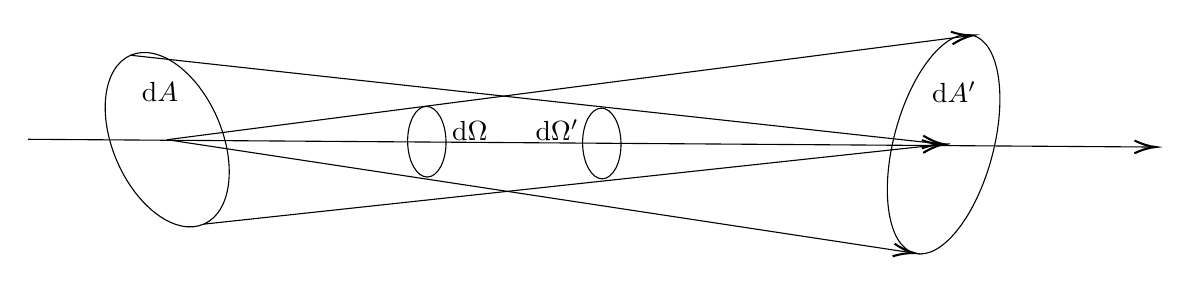
\begin{tikzpicture}[x=0.7pt,y=0.7pt,yscale=-1,xscale=1]
%Shape: Ellipse [id:dp28359105607492074] 
\draw   (77.88,155.91) .. controls (67.46,131.83) and (70.59,107.3) .. (84.87,101.12) .. controls (99.15,94.94) and (119.18,109.44) .. (129.6,133.51) .. controls (140.03,157.59) and (136.9,182.12) .. (122.61,188.3) .. controls (108.33,194.48) and (88.3,179.98) .. (77.88,155.91) -- cycle ;
%Shape: Ellipse [id:dp7012701228447336] 
\draw   (519.55,90.84) .. controls (533.29,94.51) and (537.7,122.66) .. (529.41,153.71) .. controls (521.12,184.76) and (503.26,206.97) .. (489.52,203.3) .. controls (475.78,199.63) and (471.37,171.48) .. (479.66,140.43) .. controls (487.95,109.37) and (505.81,87.17) .. (519.55,90.84) -- cycle ;
%Straight Lines [id:da8821845411756091] 
\draw    (84.87,101.12) -- (502.55,146.85) ;
\draw [shift={(504.54,147.07)}, rotate = 186.25] [color={rgb, 255:red, 0; green, 0; blue, 0 }  ][line width=0.75]    (10.93,-3.29) .. controls (6.95,-1.4) and (3.31,-0.3) .. (0,0) .. controls (3.31,0.3) and (6.95,1.4) .. (10.93,3.29)   ;
%Straight Lines [id:da5836272245786938] 
\draw    (122.61,188.3) -- (502.55,147.28) ;
\draw [shift={(504.54,147.07)}, rotate = 173.84] [color={rgb, 255:red, 0; green, 0; blue, 0 }  ][line width=0.75]    (10.93,-3.29) .. controls (6.95,-1.4) and (3.31,-0.3) .. (0,0) .. controls (3.31,0.3) and (6.95,1.4) .. (10.93,3.29)   ;
%Straight Lines [id:da12406201856368304] 
\draw    (103.74,144.71) -- (517.57,91.1) ;
\draw [shift={(519.55,90.84)}, rotate = 172.62] [color={rgb, 255:red, 0; green, 0; blue, 0 }  ][line width=0.75]    (10.93,-3.29) .. controls (6.95,-1.4) and (3.31,-0.3) .. (0,0) .. controls (3.31,0.3) and (6.95,1.4) .. (10.93,3.29)   ;
%Straight Lines [id:da3285717001142934] 
\draw    (103.74,144.71) -- (487.54,203) ;
\draw [shift={(489.52,203.3)}, rotate = 188.64] [color={rgb, 255:red, 0; green, 0; blue, 0 }  ][line width=0.75]    (10.93,-3.29) .. controls (6.95,-1.4) and (3.31,-0.3) .. (0,0) .. controls (3.31,0.3) and (6.95,1.4) .. (10.93,3.29)   ;
%Straight Lines [id:da6237274486637393] 
\draw    (32,144.5) -- (612,148.49) ;
\draw [shift={(614,148.5)}, rotate = 180.37] [color={rgb, 255:red, 0; green, 0; blue, 0 }  ][line width=0.75]    (10.93,-3.29) .. controls (6.95,-1.4) and (3.31,-0.3) .. (0,0) .. controls (3.31,0.3) and (6.95,1.4) .. (10.93,3.29)   ;
%Shape: Ellipse [id:dp851728180287646] 
\draw   (237.47,127.5) .. controls (242.94,127.41) and (247.51,135.51) .. (247.67,145.58) .. controls (247.83,155.65) and (243.53,163.89) .. (238.06,163.98) .. controls (232.58,164.07) and (228.02,155.97) .. (227.86,145.9) .. controls (227.69,135.82) and (232,127.59) .. (237.47,127.5) -- cycle ;
%Shape: Ellipse [id:dp8181356418303902] 
\draw   (327.8,128.42) .. controls (333.27,128.33) and (337.84,136.43) .. (338,146.5) .. controls (338.16,156.57) and (333.86,164.81) .. (328.38,164.9) .. controls (322.91,164.99) and (318.34,156.89) .. (318.18,146.82) .. controls (318.02,136.74) and (322.33,128.51) .. (327.8,128.42) -- cycle ;
\draw (510,120) node {$\mathrm{d}A'$};
\draw (100,120) node {$\mathrm{d}A$};
\draw (305,140) node {$\mathrm{d}\Omega'$};
\draw (260,140) node {$\mathrm{d}\Omega$};
\end{tikzpicture}
\captionsetup{justification=raggedright, singlelinecheck=false}
\caption{辐射强度不变性。}
\label{辐射强度不变性。}
\end{figure}

那么,为什么要引入立体角进行这么麻烦的定义呢?一方面,定义式中出现了法向面元$\mathrm{d}A\cos\theta$,而$\mathrm{d}A\cos\theta$相对遥远观测者会张成一个立体角。(换言之,如果要观测的对象不是一个面源,而是一个点源,辐射强度就不那么适用了。)另一方面,如此定义后辐射强度有一个非常好的性质。我们考虑一束通过恒星表面和望远镜表面两个面元的光线,如图\ref{辐射强度不变性。}所示,假定传播路径没有辐射或吸收辐射的成分起作用,通过的能量是一样的,根据辐射强度和立体角定义有
\begin{equation}
I\mathrm{d}A\cos\theta\cdot\frac{\mathrm{d}A'\cos\theta'}{r^{2}}\mathrm{d}t\mathrm{d}\nu=I'\mathrm{d}A'\cos\theta'\frac{\mathrm{d}A\cos\theta}{r^{2}}\mathrm{d}t\mathrm{d}\nu.
\end{equation}
即接收到的辐射强度就等于天体发射的辐射强度,和距离没有关系。这是个非常有用的性质,在进行星系研究的时候,因为星系离我们很远,看起来比较暗淡,往往要直接积分所有恒星的光,研究星系的面亮度。常用的辐射探测器,比如电荷耦合器件 (charge-coupled device, CCD),也是二维成像器件,它的一部分像素所记录的辐射强度,就是星系对应区域的面亮度。

此外,使用辐射强度我们还可方便地研究星光传播路径上星系介质的吸收和辐射。实验表明,辐射通过介质时,被吸收的辐射与此刻的辐射强度本身和辐射通过的单位距离成正比,即
\begin{equation}
\mathrm{d}I_{\nu}\propto{}I_{\nu}\left(l\right)\mathrm{d}l,
\end{equation}
一般记比例系数为$\alpha_{\nu}$.量纲分析发现$\alpha_{\nu}^{-1}$是一个长度量,我们定义$l=\alpha_{\nu}^{-1}$为光子的平均自由程。一般来讲$\alpha_{\nu}=n\sigma$, $n$是粒子数密度,$\sigma$是粒子与光子的散射截面。

此外介质本身可能也有发光能力,但这是介质本身的性质,和通过介质的辐射无关,记其为$j_{\nu}$即可,表征的是介质单位体积单位立体角单位频率间隔单位时间辐射出的能量
\begin{equation}
\mathrm{d}E_{\nu}=j_{\nu}\mathrm{d}V\mathrm{d}\Omega\mathrm{d}\nu\mathrm{d}t.
\end{equation}

于是我们可以得到辐射转移方程
\begin{equation}
\frac{\mathrm{d}I_{\nu}}{\mathrm{d}l}=j_{\nu}-\alpha_{\nu}I_{\nu}.
\end{equation}
假设介质不发光,即$j_{\nu}=0$,容易解得
\begin{equation}
I_{\nu\text{obs}}=I_{\nu0}\mathrm{e}^{-\int\alpha_{\nu}\mathrm{d}l},\label{1.1.13}
\end{equation}
由此我们可以定义光学深度(简称光深)
\begin{equation}
\mathrm{d}\tau_\nu=\alpha_{\nu}\mathrm{d}l,\\
\end{equation}
此时 (\ref{1.1.13}) 式改写为
\begin{equation}
I_{\nu\text{obs}}=I_{\nu0}\mathrm{e}^{-\tau_{\nu}},\label{1.1.15}
\end{equation}
因此光深表征了介质的吸收能力。

由于吸收系数和发射系数都是介质本身的性质,我们更倾向于将二者写在一起。为此引入源函数 (Source Function)
\begin{equation}
S_{\nu}=\frac{j_{\nu}}{\alpha_{\nu}},
\end{equation}
辐射转移方程改写为
\begin{equation}
\frac{\mathrm{d}I_{\nu}}{\mathrm{d}\tau_{\nu}}=S_{\nu}-I_{\nu},
\end{equation}
它的形式解为
\begin{equation}
I_{\nu\text{obs}}=I_{\nu0}\mathrm{e}^{-\tau_{\nu}}+\int^{\tau_{\nu}}_{0}S_{\nu}\left(t_{\nu}\right)\mathrm{e}^{-\left(\tau_{\nu}-t_{\nu}\right)}\mathrm{d}t_{\nu}.
\end{equation}
即观测到的辐射一部分来自背景辐射$I_{\nu}\left(0\right)$,另一部分来自背景辐射所穿过的介质$S_{\nu}$.

如果源函数与光深无关(即沿辐射传播路径源函数是常数),形式解改写为
\begin{align}
I_{\nu\text{obs}}&=I_{\nu0}\mathrm{e}^{-\tau_{\nu}}+S_{\nu}\int^{\tau_{\nu}}_{0}\mathrm{e}^{-\left(\tau_{\nu}-t_{\nu}\right)}\mathrm{d}t_{\nu}.\notag\\
&=I_{\nu0}\mathrm{e}^{-\tau_{\nu}}+S_{\nu}\left(1-\mathrm{e}^{-\tau_{\nu}}\right).
\end{align}
习惯上称$\tau_{\nu}\gg1$时为光学厚,$\tau_{\nu}\ll1$时为光学薄。根据上式可知,介质光学厚时所观测到的辐射强度就是介质的源函数。此外我们将在后续说明,源函数往往与介质的温度有关。而介质光学薄时所观测到的辐射强度为$I_{\nu0}+S_{_{\nu}}\tau_{\nu}$,因此如果我们先前就对背景辐射有较为明确的了解,可借此研究介质的光深,而$\mathrm{d}\tau_{\nu}=\alpha_{\nu}\mathrm{d}l=n\sigma\mathrm{d}l$,进一步可了解介质的密度。

\subsubsection{测光系统和星等系统}
前文提到立体角的引入与面元有关。辐射强度的定义用到面元的优点是,很容易建立辐射强度与亮度的关系,这也是我们最初的目的之一。只要对立体角做积分(要对整个$4\pi$积分,因为面元可以通过来自四面八方的辐射)就能得到自面元两侧方向穿过面元的能量的差额(如向左$10\,\mathrm{J}$向右$20\,\mathrm{J}$合计向右$10\,\mathrm{J}$):
\begin{equation}
E_{\nu}=\int_{\Omega}I_{\nu}\cos\theta\mathrm{d}A\mathrm{d}t\mathrm{d}\nu\mathrm{d}\Omega,
\end{equation}
进一步就可知道单位时间单位面积单位频率间隔所通过的“净能量”(即差额)为
\begin{equation}
F_{\nu}=\int_{\Omega}I_{\nu}\cos\theta\mathrm{d}\Omega.
\end{equation}
我们称其为流量密度 (Flux Density).在一定频率范围内积分得到
\begin{equation}
F=\int_{\nu_{1}}^{\nu_{2}}F_{\nu}\mathrm{d}\nu.\label{1.1.22}
\end{equation}
我们称其为流量 (Flux),它所表征的正是天体在某一波段内的亮度。

建立了辐射强度与亮度的关系后,我们就可以研究光深对星等的影响。遥远天体的辐射经常会受到星际介质吸收和散射的影响,改变辐射的分布和强度,这被称作星际消光。在可见光和红外区,$\alpha_{\nu}\propto{}\nu$,即频率越高(波长越短)消光越厉害,从而使天体变红。另一方面天体会变暗,根据 (\ref{1.1.15}) 式可知星等会多一项
\begin{equation}
m_{\nu}'=m_{\nu}+A_{\nu}=m_{\nu}-2.5\log_{10}\left(\mathrm{e}^{-\tau_{\nu}}\right).
\end{equation}

现在我们继续研究 (\ref{1.1.22}) 式。一个很自然的想法是,在望远镜里塞各种滤光片就能得到不同波段范围内的亮度。由此我们定义色指数,为某一短波段的视星等减去某一长波段的视星等。由于星等相减消去了距离因素,故色指数不需要测距也能直接使用。(如果不同波段消光程度相同的话。)

前文已经提到过恒星的辐射可以近似地用黑体辐射来表示,即
\begin{equation}
I_{\nu}=B_{\nu}\left(T\right)=\frac{2h\nu^{3}}{c^{2}}\frac{1}{\mathrm{e}^{\frac{h\nu}{k_{\text{B}}T}}-1},
\end{equation}
可见随着温度变化,辐射强度随频率的分布也会发生变化。一方面会体现在色指数上。温度较高,辐射会集中在频率较高的地方,色指数就较低。有各种经验公式
\begin{equation}
T=\frac{7300\,\mathrm{K}}{\mathrm{B-V}+0.6},T=\frac{7090\,\mathrm{K}}{\mathrm{B-V}+0.71},T=\frac{8450\,\mathrm{K}}{\mathrm{B-V}+0.865},
\end{equation}
其中 B, V 指代 B 波段和 V 波段测得的星等,一些常见波段如表\ref{常用滤光片波段。}所示。另一方面则会体现在峰值频率的移动,通过对以波长(而非频率)和温度为自变量的黑体辐射公式求导容易得出
\begin{equation}
\lambda_{\max}T=2.9\times10^{6}\,\mathrm{nm\cdot K},
\end{equation}
这被称作维恩位移定律,是温度和辐射峰值波长所满足的关系。具体可见图\ref{黑体辐射峰值随温度的变化。}所示。

\begin{figure}[!htbp]
\centering
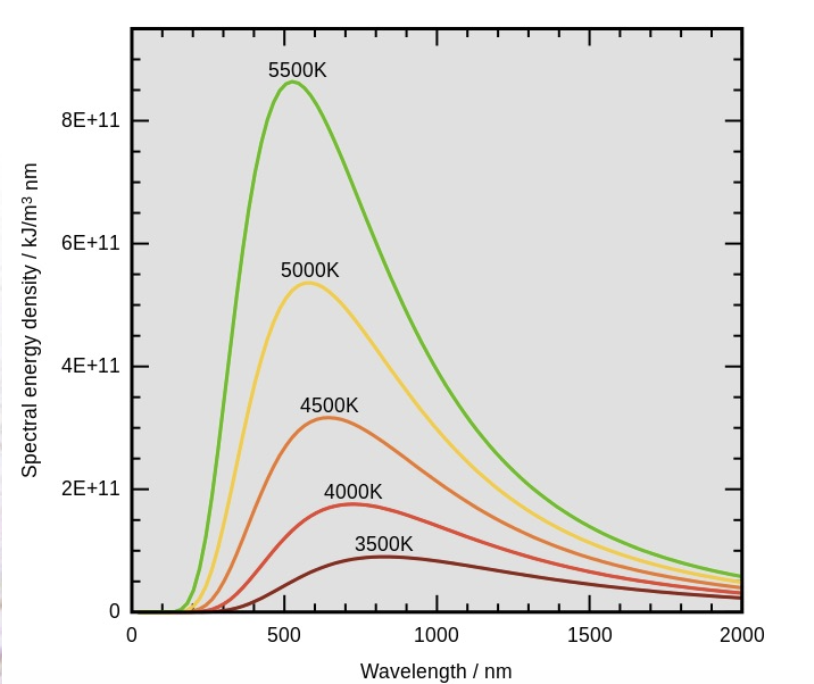
\includegraphics[width=10cm]{figures/figure1_1.png}
\captionsetup{justification=raggedright, singlelinecheck=false}
\caption{黑体辐射峰值随温度的变化。}
\label{黑体辐射峰值随温度的变化。}
\end{figure}

\begin{table}[htbp]
\centering
\caption{常用滤光片波段。}
\begin{tabular}{c c c c c c c c c c c c}
\hline
 & U & B & V & R & I & J & H & K & L & M & N\\
\cline{1-12}
$\lambda\left(\si{\angstrom}\right)$ & 3650 & 4400 & 5500 & 7000 & 9000 & 12500 & 16500 & 22000 & 36000 & 48000 & 104000\\
\cline{1-12}
$\Delta{}\lambda\left(\si{\angstrom}\right)$ & 680 & 980 & 890 & 2200 & 2400 & 3800 & 4000 & 6000 & 12000 & 8000 & 60000\\
\cline{1-12}
\end{tabular}
\label{常用滤光片波段。}
\end{table}

此处可能有读者会疑惑为什么不用$L=4\pi R^{2}\sigma_{\text{SB}}T^{4}$求温度,因为恒星离我们过于遥远,很难通过观测分辨其大小,即使能做到也很浪费观测资源,应该要反过来用这个公式求半径才对。

我们注意到表\ref{常用滤光片波段。}中有一栏为$\Delta{}\lambda$,这个量又是如何定义的?首先对于滤光片,我们用带通 (Bandpass) 表征波长$\lambda$处透过光的比例,取值范围$0\le T_{\text{BP}}(\lambda)\le 1$,光可以完全透过滤光片时$T_{\text{BP}}$取 1. $\Delta\lambda$为滤光片带宽,是$T_{\text{BP}}=0.5$所对应的两个波长的差值。习惯上用宽带 ($\Delta\lambda>30\,\mathrm{nm}$) 滤光片进行暗弱天体测光,或者粗略测量辐射的频率分布(连续谱),用窄带 ($\Delta\lambda<10\,\mathrm{nm}$) 滤光片测量吸收和发射谱线轮廓,中带滤光片带宽则介于二者之间。

采用不同的滤光片组合我们可以得到不同的测光系统。所谓测光,就是用辐射探测器配合望远镜测定天体的亮度。常用的有 UBVRI(紫外、蓝、可见、红、红外)五色测光系统,$m_{\text{pg}},m_{\text{pv}}$二色测光系统,uvby 四色测光系统等。我们简单介绍一下后面两者吧。在各种光电器件(使用光电效应测光的器件)还没发明的时候,人类使用照相底片拍摄天区,于是有了照相星等$m_{\text{pg}}$;另一方面则使用正色片前加黄滤光片测光得到仿视星等$m_{\text{pv}}$(类似目视星等),如此以来便得到最初的色指数。uvby 四色系统波段则如表\ref{uvby 四色测光滤光片波段。}所示。我们发现 uvby 的带宽较 UVBRI 测光系统更窄一点,主要用来测吸收线。uvby 主要使用三个参数进行分析。首先$\text{b}-\text{y}$与$\text{B}-\text{V}$相当,只与恒星温度有关。接着是$C_{1}=\left(\text{u}-\text{v}\right)-\left(\text{v}-\text{b}\right)$,与 Balmer Break(我们后续会解释这是什么)有关。最后是$m_{1}=\left(\text{v}-\text{b}\right)-\left(\text{b}-\text{y}\right)$,与恒星金属丰度有关。

\begin{table}[htbp]
\centering
\caption{uvby 四色测光滤光片波段。}
\begin{tabular}{c c c c c}
\hline
 & u & v & b & y\\
\cline{1-5}
$\lambda\left(\si{\angstrom}\right)$ & 3500 & 4100 & 4670 & 5470\\
\cline{1-5}
$\Delta{}\lambda\left(\si{\angstrom}\right)$ & 300 & 190 & 180 & 230\\
\cline{1-5}
\end{tabular}
\label{uvby 四色测光滤光片波段。}
\end{table}

最后我们来定义星等系统的零点。有两种常用的方式:

- Vega Magnitude System: 织女星在所有滤光片中的视星等(注意,不是绝对星等)为 0.织女星不同波段的亮度肯定是不同的,因此不同波段相同星等所对应的亮度也是不同的。如果一颗恒星 V 波段星等是$5.4$等,B 波段星等是$4.2$,并不一定意味着 B 波段流量更高。

- AB Magnitude System: 早期用 Vega 星等是因为观测中用标准星定标比较方便和准确,但后来观测精度提高,织女星流量测得更加准确,零点就发生了漂移。同时观测波段也有拓展,紫外红外波段没有合适的标准星,于是不如将各个波段所使用的流量零点统一,取流量零点为常数$\langle F_{\text{V},m=0}\rangle=3631\times10^{-23}\,\mathrm{erg\cdot s^{-1}\cdot cm^{-2}\cdot Hz^{-1}}$.这个值的来源是织女星在 V 波段的流量。注意,$\langle{}F_{\text{V},m=0}\rangle$量纲最后一项是$\mathrm{Hz}^{-1}$,我们认为单位频率间隔和单位波长间隔满足
\begin{align}
\nu&=\frac{c}{\lambda},\\
\mathrm{d}\nu&=-\frac{c}{\lambda^{2}}\mathrm{d}\lambda,
\end{align}
因此如果用波长为单位来描述流量零点,
\begin{align}
F_{\lambda}=F_{\nu}\left\vert{}\frac{\mathrm{d}\nu}{\mathrm{d}\lambda}\right\vert{}=\frac{c}{\lambda^{2}}F_{\nu},
\end{align}
零点并不是一个常数,会随波长变化而变化。前文维恩位移定律强调对波长求导也是出于这个原因。如果有心计算,会发现相同温度下,黑体辐射峰值波长和峰值频率相乘并不等于光速,原因就在于$\mathrm{d}\nu$和$\mathrm{d}\lambda$的划分并非线性对应,能量在$\mathrm{d}\nu$和$\mathrm{d}\lambda$中的分配是不一样的。

而 AB 星等则定义为
\begin{align}
m_{\mathrm{BP}}&=-2.5\log_{10}(\frac{\langle F_{\mathrm{BP}}\rangle}{\langle F_{\text{V},m=0}\rangle}),\\
\langle F_{\mathrm{BP}}\rangle&=\frac{\int T_{\mathrm{BP}}(\lambda)F_{\text{obj}}(\lambda)\mathrm{d}\lambda}{\int T_{\mathrm{BP}}(\lambda)\mathrm{d}\lambda}.
\end{align}

滤光片测得的光度(去除距离因素后)都是某一波段内的光度,如果对全波段积分就得到了天体的总光度(或称热光度)。前文给出的$L_{\odot}$就是太阳的总光度。总光度对应的星等被称作热星等。热星等自然也是一种绝对星等。按照定义,总光度观测要求得到天体在整个电磁波段的辐射,但实际观测中,大气吸收使我们在地面上只能观测到光学、近红外、射电波段的信号,同时强度也有所减弱,全波段测量困难。因此没法通过观测确定天体的热星等。常见方法是在$M_{\text{V}}$加上一个改正值(热改正)得到“真实”的热星等。热星等也需要流量零点,定标方法为将太阳热星等定作$M_{\mathrm{bol},\odot}=4.76$,对应的热改正$\mathrm{BC}_{\odot}=M_{\mathrm{V},\odot}-M_{\mathrm{bol},\odot}=0.07$.一般来讲较热和较冷的恒星热改正大(辐射集中在 V 波段两侧),中间区间的恒星热改正小(辐射本就集中在 V 波段)。

\subsubsection{描述辐射场的其他物理量}
本小节我们将通过辐射强度构建一些描述辐射场的物理量。

首先我们介绍一种辐射强度的等价描述方法。我们已经知道辐射强度是用通过面元的能量来定义的,实际上这种能量也可以用通过面元的光子来描述。定义辐射场单位体积中光子数为$f_{R}\left(\vec{r},\vec{m},\nu,t\right)$,单位时间内通过面元的体积为$\mathrm{d}A\cos\theta c\mathrm{d}t$,光子所携带的能量为
\begin{equation}
\mathrm{d}E_{\nu}=h\nu\cdot f_{R}\left(\vec{r},\vec{m},\nu,t\right)\left(\mathrm{d}A\cos\theta\mathrm{d}\Omega\mathrm{d}\nu c\mathrm{d}t\right),
\end{equation}
对照得到
\begin{equation}
I_{\nu}\left(\vec{r},\vec{m},t\right)=ch\nu f_{R}\left(\vec{r},\vec{m},\nu,t\right).
\end{equation}
其中$\vec{r}$是面元坐标,$\vec{m}$是光线传播方向。

将$I_{\nu}$对方向做平均可以得到平均辐射强度:
\begin{equation}
J_{\nu}=\frac1{4\pi}\int_{4\pi}I_{\nu}\mathrm{d}\Omega,
\end{equation}

接着定义辐射流矢量
\begin{equation}
\vec{\mathcal{F}_{\nu}}(\vec{r},t)=\int_{4\pi}I_{\nu}\left(\vec{r},\vec{m},t\right)\vec{m}\mathrm{d}\Omega,
\end{equation}
它与流量的关系为
\begin{equation}
F_{\nu}=\vec{\mathcal{F}_{\nu}}\cdot\vec{n}.
\end{equation}
其中$\vec{n}$是面元法向。

辐射穿过单位体积元所用的时间为$\mathrm{d}t=\dfrac{\mathrm{d}l\sec\theta}{c}$,该单位时间中还保留着能量
\begin{align}
\mathrm{d}E_{\nu}&=I_\nu\left(\vec{r},\vec{m},t\right)\mathrm{d}A\cos\theta\mathrm{d}\Omega\mathrm{d}\nu\mathrm{d}t\notag\\
&=\frac{1}{c}I_\nu\left(\vec{r},\vec{m},t\right)\mathrm{d}V\mathrm{d}\Omega\mathrm{d}\nu.
\end{align}
总计所有方向积分就得到体元从各个方向得到的能量。定义辐射密度
\begin{equation}
U_{\nu}=\frac1c\int_{4\pi}I_{\nu}\mathrm{d}\Omega=\frac{4\pi}{c}J_{\nu},
\end{equation}
表示通过辐射场内某处单位体积单位频率间隔的辐射能。

有能量自然要考虑动量。单位辐射能光子携带动量的法向分量为
\begin{equation}
\mathrm{d}p_{n}=\frac{\mathrm{d}E_{\nu}}{c}\cos\theta=\frac{1}{c}I_{\nu}\cos^{2}\theta\mathrm{d}\Omega\mathrm{d}\nu\mathrm{d}A\mathrm{d}t.
\end{equation}
进而可以根据单位面积单位频率间隔面元受力定义辐射压力
\begin{equation}
P_{R,\nu}=\frac1c\int_{4\pi}I_{\nu}\cos^{2}\theta\mathrm{d}\Omega,
\end{equation}
即单位频率间隔施加于面元的压强。它本质是个二阶对称张量
\begin{align}
\overset{\rightharpoonup\!\!\!\rightharpoonup}{P}_{R,\nu}\left(\vec{r},t\right)&=\frac{1}{c}\int_{4\pi}I_\nu\left(\vec{r},\vec{m},t\right)\vec{m}\vec{m}\mathrm{d}\Omega,\\
P&=\left[\overset{\rightharpoonup\!\!\!\rightharpoonup}P\cdot\vec n\right]\cdot\vec n.
\end{align}
分量形式
\begin{equation}
\overset{\rightharpoonup\!\!\!\rightharpoonup}P_{ij}=\frac{1}{c}\int_{4\pi}I_{\nu}m_{i}m_{j}\mathrm{d}\Omega,
\end{equation}

但更多时候我们并不关心压力的压强效果,而是关心压力所带来的加速度,因此有必要考虑介质的质量,为此先通过吸收系数定义质量吸收系数(或称不透明系数)
\begin{equation}
\kappa_\nu=\frac{\alpha_\nu}\rho=\frac{n\sigma_{\nu}}{\rho}=\frac{\sigma_\nu}{m}.
\end{equation}
介质吸收某一辐射$I_{\nu}\left(\vec{m}\right)$在$\vec n$方向得到的动量为$\dfrac{1}{c}\left(\alpha_\nu I_\nu\mathrm{d}l\right)\mathrm{d}A\mathrm{d}\Omega\mathrm{d}\nu\mathrm{d}t\vec{m}\cdot\vec{n}$,积分得到
\begin{align}
\vec{F}\mathrm{d}t&=\int_{\nu}\mathrm{d}\nu\int_{\Omega}\mathrm{d}\Omega\vec{m}\cdot\vec{n}\left[\frac{1}{c}\left(\alpha_{\nu}I_{\nu}\mathrm{d}l\right)\mathrm{d}A\mathrm{d}t\right]\notag\\
&=\int_{\nu}\mathrm{d}\nu\int_{\Omega}\mathrm{d}\Omega\vec{m}\cdot\vec{n}\cdot\left[\frac{1}{c}\left(\kappa_{\nu}\frac{m}{\mathrm{d}l\mathrm{d}A}I_{\nu}\mathrm{d}l\right)\mathrm{d}A\mathrm{d}t\right]\notag\\
&=\frac{1}{c}m\mathrm{d}t\int_{\nu}\kappa_{\nu}F_{\nu}\mathrm{d}\nu.
\end{align}
由此得到辐射场中单位质量受力(加速度)为
\begin{equation}
\vec{f}=\frac{\vec{F}}{m}=\frac{1}{c}\int\kappa_{\nu}\vec{F}_{\nu}\mathrm{d}\nu.
\end{equation}
在球对称辐射场中常写作
\begin{equation}
f=\frac{1}{c}\kappa F=\frac{1}{c}\kappa\dfrac{L}{4\pi R^2}=\frac{L\sigma}{4\pi R^{2}cm}.
\end{equation}
可见介质受辐射力所得到的加速度取决于辐射源光度、介质散射截面大小(越大相当于面积越大,能接收到的光子越多)、介质到辐射源的距离以及介质质量。

于是我们自然地引出 Eddington 光度。星系中心的超大质量黑洞,吸积物质时可以将物质的引力能转化为辐射能。当黑洞的引力与辐射力达到平衡时,吸积率就不能再上升,此时有最大光度。假设被吸积的物质为纯氢气体,散射截面为汤姆孙散射截面$\sigma_{\text{T}}=6.65\times10^{-25}\,\mathrm{cm}^{2}$,此时最大光度被称作 Eddington 光度:
\begin{align}
\frac{\mathrm{G}M_{\text{BH}}}{R^{2}}&=\frac{L\sigma}{4\pi R^{2}cm},\\
L_{\text{Edd}}&=\frac{4\pi c\mathrm{G}M_{\text{BH}}m_{\mathrm{H}}}{\sigma_{\text{T}}}=1.25\times10^{38}\frac{M_{\text{BH}}}{M_\odot}\,\mathrm{erg\cdot{}s^{-1}}.
\end{align}
球对称吸积并不常见,大多数情况下吸积物质会形成一个盘,因此与盘呈一定夹角的辐射并不能有效转换为对物质的推力,因此可以实现超 Eddington 吸积。但随着黑洞质量逐渐提高,它的吸积能力可能会不断下降,一般超大质量黑洞辐射功率仅能达到 Eddington 光度的百分之一。但与太阳光度$L_{\odot}=3.86\times10^{33}\,\mathrm{erg\cdot s^{-1}}$对比,黑洞吸积能释放的辐射依旧是巨大的。

\subsubsection{洛伦兹不变量}
众所周知,我们所身处的宇宙是在不断膨胀的,且距离我们越远的空间中的天体退行速度越快。学过广义相对论的我们自然要考虑这么一个问题:这些天体辐射出的光是什么样子的呢?接下来我们将改写辐射转移方程的形式,开始研究辐射场中不随洛伦兹变换而发生变化的物理量,解答这个问题的一小部分。

注意到$\mathrm{d}t=\dfrac{\mathrm{d}l}c$,辐射强度沿光线传播方向的变化可以写作
\begin{align}
I_{\nu}\left(\vec{r}+\mathrm{d}\vec{r},t+\mathrm{d}t\right)&=I_\nu\left(\vec r,t\right)+\left(\frac{\partial I_\nu}{\partial t}\mathrm{d}t+\frac{\partial I_\nu}{\partial l}\mathrm{d}l\right)\notag\\
&=I_\nu\left(\vec r,t\right)+\left(\frac1c\frac{\partial}{\partial t}+\frac{\partial}{\partial l}\right)I_\nu \mathrm{d}l.
\end{align}
因此辐射转移方程可以写作
\begin{equation}
\left(\frac{1}{c}\frac{\partial}{\partial t}+\frac{\partial}{\partial l}\right)I_\nu\left(\vec r,t\right)=j_\nu-\alpha_\nu I_\nu\left(\vec{r},t\right).\label{1.1.51}
\end{equation}
洛伦兹变换下,$t,I_{_{\nu}},j_{\nu},\alpha_{\nu}$等都可能发生变化,我们并不确定换系后辐射转移方程是否还成立,因此要逐个分析各个物理量的变化。

首先确定频率、辐射方向随参考系变换的变化。依旧遵循惯例,在$x\text{\textendash}y\text{\textendash}z$直角坐标系中取经角$\varphi$,纬角$90^{\circ}-\theta$,光子运动方向为
\begin{equation}
\left(n_x,n_y,n_z\right)=\left(\cos\varphi\sin\theta,\sin\varphi\sin\theta,\cos\theta\right).
\end{equation}
虽然听起来有点离谱,但此处我们采用$ict$“度规”,取$x^{1}=x,x^{2}=y,x^{3}=z,x^{4}=ict,\beta=\dfrac{v}{c},\gamma=\dfrac{1}{\sqrt{1-\dfrac{v^2}{c^2}}}$,光子四维动量写作
\begin{equation}
p=\frac{h\nu}{c}
\begin{pmatrix}
n_x,n_y,n_z,i
\end{pmatrix}.
\end{equation}
按照惯例面元法向方向是$z$轴方向,因此洛伦兹变换写作
\begin{equation}
\begin{pmatrix}
\nu' n'_z\\\nu' n'_y\\\nu' n'_x\\\nu' i
\end{pmatrix}=
\begin{pmatrix}
\gamma & 0 & 0 & i\gamma\beta\\
0 & 1 & 0 & 0\\
0 & 0 & 1 & 0\\
-i\gamma\beta & 0 & 0 &\gamma
\end{pmatrix}
\begin{pmatrix}
\nu n_z\\\nu n_y\\\nu n_x\\\nu i
\end{pmatrix},
\end{equation}
解得
\begin{align}
\cos\theta'&=\frac{\cos\theta-\beta}{1-\cos\theta\beta}.\\
\nu'&=\gamma\nu\left(1-\cos\theta\beta\right).\\
\varphi'&=\varphi.
\end{align}
进而可以推得
\begin{align}
\frac{\mathrm{d}\nu'}{\mathrm{d}\nu}&=\gamma\left(1-\cos\theta\beta\right)=\frac{\nu'}{\nu},\\
\mathrm{d}\cos\theta'&=\left(\frac{\nu}{\nu'}\right)^2\mathrm{d}\cos\theta.
\end{align}
注意到
\begin{equation}
\mathrm{d}\Omega=\sin\theta\mathrm{d}\theta\mathrm{d}\varphi=-\mathrm{d}\cos\theta\mathrm{d}\varphi,
\end{equation}
可知
\begin{equation}
\nu\mathrm{d}\nu\mathrm{d}\Omega=\nu'\mathrm{d}\nu'\mathrm{d}\Omega'.
\end{equation}
于是我们得到了第一个洛伦兹不变量。

为了得到其他的洛伦兹不变量,我们势必要考虑辐射场中的标量。容易想到的自然是光子数。一定时间内通过同一面元的光子数是一定的。在一个相对面元静止的参考系中,
\begin{equation}
\mathrm{d}N=\frac{1}{h\nu}I\left(\cos\theta,\nu\right)\mathrm{d}A\cos\theta\mathrm{d}\Omega\mathrm{d}\nu \mathrm{d}t,
\end{equation}
换系后则要添加一项,面元扫过的区域中所含的光子数:
\begin{align}
\mathrm{d}N'&=\frac{1}{h\nu'}I'\left(\cos\theta',\nu'\right)\mathrm{d}A\cos\theta'\mathrm{d}\Omega'\mathrm{d}\nu' \mathrm{d}t'+f_{R}'\left(\vec{r'},\nu',t'\right)v\mathrm{d}t'\mathrm{d}A\mathrm{d}\Omega'\mathrm{d}\nu'\notag\\
&=\frac{1}{h\nu'}I'\left(\cos\theta',\nu'\right)\mathrm{d}A\mathrm{d}\Omega'\mathrm{d}\nu'\mathrm{d}t'\left(\frac{v}{c}+\cos\theta'\right),
\end{align}
联立方程,配出$\nu\mathrm{d}\nu\mathrm{d}\Omega$形式得到
\begin{equation}
\frac{1}{\nu^2}I_{\nu}\cos\theta\mathrm{d}t=\frac{1}{\nu'^2}I_{\nu'}'\mathrm{d}t'\left(\frac{v}{c}+\cos\theta'\right).
\end{equation}
根据对称性写出
\begin{align}
\mathrm{d}t'&=\gamma\mathrm{d}t,\\
\cos\theta&=\dfrac{\cos\theta'+\beta}{1+\cos\theta'\beta},\\
\nu&=\gamma\nu'\left(1+\cos\theta'\beta\right),
\end{align}
最终得到
\begin{equation}
\frac{I_{\nu}}{\nu^3}=\frac{I_{\nu'}'}{\nu'^3}.
\end{equation}
因此辐射强度和频率三次方成正比。辐射源靠近我们运动时,我们所观测到的频率会变高,上式告诉我们辐射强度会增强,反之变弱。实际观测中我们确实发现了该效应所引起的现象。超大质量黑洞吸积时会在两极产生喷流,但多数时候只能观测到一支喷流,原因就是另一支的物质远离我们运动,难以观测到。

接着我们来研究发射系数和吸收系数的变化。同样考虑光子数,同一体元$dV$发射的光子数是一定的:
\begin{equation}
\frac{j_\nu\mathrm{d}V\mathrm{d}\Omega\mathrm{d}\nu\mathrm{d}t}{h\nu}=\frac{j_\nu'\mathrm{d}V'\mathrm{d}\Omega'\mathrm{d}\nu'\mathrm{d}t'}{h\nu'},
\end{equation}
注意到$\mathrm{d}V\mathrm{d}t=\mathrm{d}V'\mathrm{d}t',\nu\mathrm{d}\nu\mathrm{d}\Omega=\nu'\mathrm{d}\nu'\mathrm{d}\Omega'$,得到
\begin{equation}
\frac{j_\nu}{\nu^2}=\frac{j_\nu'}{\nu'^2}.
\end{equation}
而吸收系数满足$\alpha_{\nu}=\dfrac{j_{\nu}}{S_{\nu}}$,因此我们直接写出
\begin{equation}
\alpha_{\nu}\nu=\alpha'_{\nu'}\nu'.
\end{equation}
所需要的洛伦兹不变量都已得到,现在可以写出运动系下辐射转移方程的形式。首先写出算符$\left(\dfrac{1}{c}\dfrac{\partial{}}{\partial{}t}+\dfrac{\partial{}}{\partial{}l}\right)$的变化
\begin{equation}
\begin{pmatrix}
\dfrac{\partial}{\partial z}\\
\dfrac{\partial}{\partial x}\\
\dfrac{\partial}{\partial y}\\
\dfrac1{ic}\dfrac{\partial}{\partial t}\\
\end{pmatrix}
=L^{-1}
\begin{pmatrix}
\dfrac{\partial}{\partial z'}\\
\dfrac{\partial}{\partial x'}\\
\dfrac{\partial}{\partial y'}\\
\dfrac1{ic}\dfrac{\partial}{\partial t'}\\
\end{pmatrix}
=\begin{pmatrix}
\gamma(\dfrac{\partial}{\partial z'}-\dfrac{\beta}c\dfrac{\partial}{\partial t'})\\
\dfrac{\partial}{\partial x'}\\
\dfrac{\partial}{\partial y'}\\
\dfrac\gamma{ic}(\dfrac{\partial}{\partial t'}-c\beta\dfrac{\partial}{\partial z'})\\
\end{pmatrix},
\end{equation}
\begin{equation}
\frac1c\frac{\partial }{\partial t}+n_{x}\frac{\partial}{\partial x}+n_{y}\frac{\partial}{\partial y}+n_{z}\frac{\partial}{\partial z}=\frac{\nu'}{\nu}[\frac1c\frac{\partial}{\partial t'}+n_{x}'\frac{\partial}{\partial x'}+n_{y}'\frac{\partial}{\partial y'}+n_{z}'\frac{\partial}{\partial z'}].
\end{equation}
注意到有$\dfrac{\nu'}{\nu}$这个因子,再将前文得到的$I'_{\nu'},j'_{\nu'},\alpha'_{\nu'}$代入 (\ref{1.1.51}) 式,容易发现运动系中辐射转移方程的形式并未改变。

\newpage
\subsection{偏振光的描述}
好消息,我们对电磁辐射强度的研究告一段落了。由于电磁波是一种横波,我们接下来就要研究它的相位带来的影响了。

\subsubsection{基本原理}
\begin{figure}[!htbp]
\centering
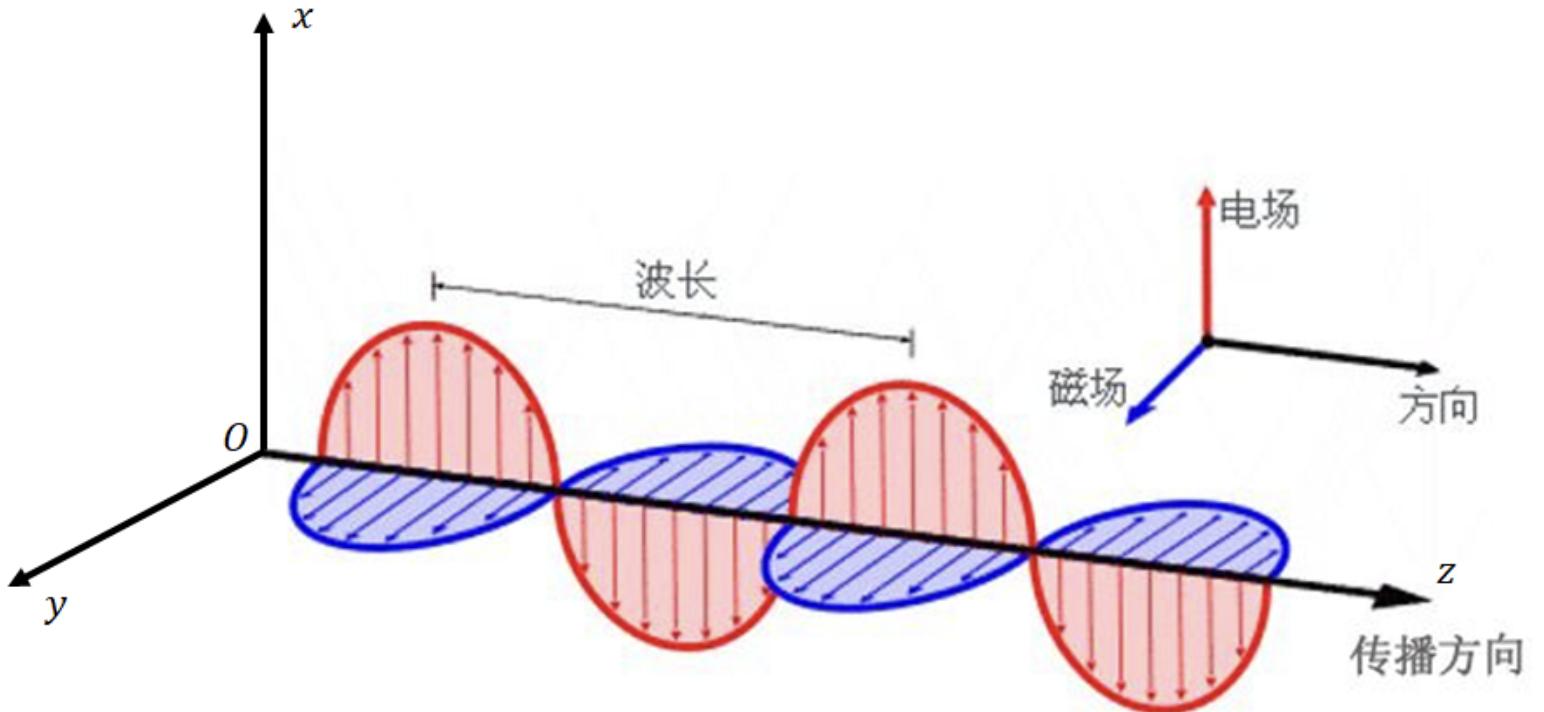
\includegraphics[width=10cm]{figures/figure1_2.png}
\captionsetup{justification=raggedright, singlelinecheck=false}
\caption{电磁波的电矢量。}
\label{电磁波的电矢量。}
\end{figure}

我们知道电磁场的电矢量位于垂直于传播方向的平面上,它的指向可以取该平面内的任意一个方向。如果一束光内的电矢量振动方向都沿着某个确定的方向,不随时间变化,它被称作线偏振光。

那么,如果一束光由两束电矢量振动方向不同的线偏振光叠加会发生什么呢?有这么一种可能,两束光的相位有所差异,一束光电矢量最大时另一束最小,反之亦然,因此合成出的电矢量指向会发生变化。因为电矢量的振动是简谐运动,合成后的电矢量会以某个确定的角速度旋转。按旋转方向可以将其分为左旋偏振光和右旋偏振光。
\begin{figure}[!htbp]
\centering
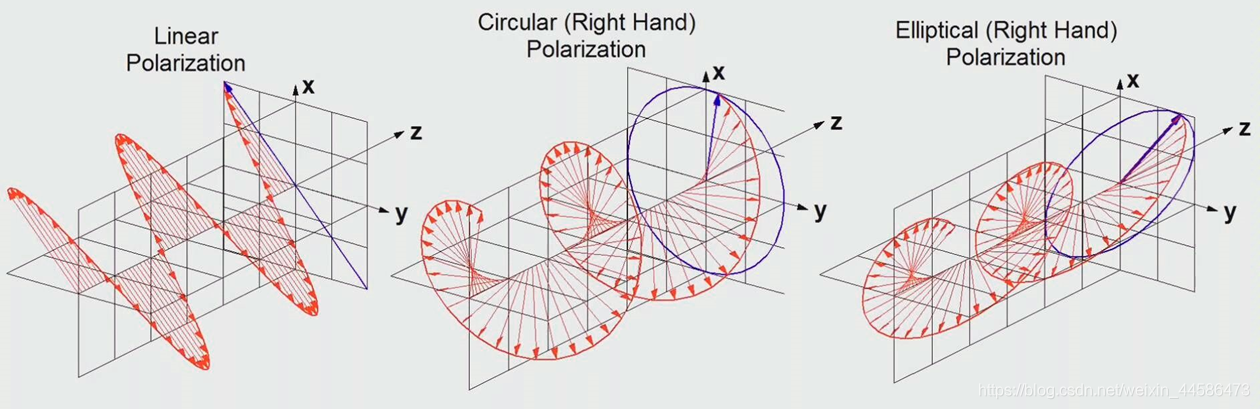
\includegraphics[width=17cm]{figures/figure1_3.png}
\captionsetup{justification=raggedright, singlelinecheck=false}
\caption{右旋偏振光示意图。}
\label{右旋偏振光示意图。}
\end{figure}

介绍一下如何判断左旋和右旋。如图$\ref{右旋偏振光示意图。}$所示,光朝$z$轴正方向传播,传播路径上放置一个$x\text{\textendash}y$平面。以右旋偏振光为例,随着光线向前推进,电矢量在$x\text{\textendash}y$平面上顺时针转动,右手四指沿着转动方向绕转,大拇指指向传播方向,故称其为右旋。

我们容易发现,如果两束线偏振光振幅相同,相位刚好相差$90^{\circ}$,那么电矢量末端在$x\text{\textendash}y$平面上一定时间内绘制出的轨迹恰好是一个圆,并且旋转角速度固定。称为圆偏振光。而如果振幅不同,或者相位差取其他值,则会绘制出一个椭圆,称为椭圆偏振光。

自然界中的辐射肯定不是单纯的两束线偏振光的集合。如太阳辐射到地球的自然光,电矢量在各个方向振动几率相等、平均振幅相等,称其为非偏振光。有时,电矢量在某个方向上占优,与之垂直的方向上强度最小,可看作是非偏振光和偏振光的叠加,称其为部分偏振光。实际观测中大部分电磁辐射都是部分偏振光。

我们可以用偏振度$\Pi$来区分(完全)偏振光、部分偏振光和非偏振光,其定义为偏振部分强度与总强度之比,
\begin{equation}
\Pi=\dfrac{\sqrt{Q^2+U^2+V^2}}I=\frac{I_{\text{pol}}}{I}.
\end{equation}
式中$I,Q,U,V$被称作 Stokes 参数,其具体含义我们将在下一小节介绍。

有很多物理机制能产生偏振光。首先,光在固体、液体表面反射后能产生偏振光,喜欢摄影的同学们应该很了解这一点。实际观测中,行星表面反射的光就是偏振光。其次,电子、分子、尘埃等物质的散射能产生高度线偏振光,偏振方向与散射面垂直,偏振度由散射角决定。尘埃的多次散射可以产生圆偏振。比如木星大气两极有明显的偏振,主要由气溶胶颗粒散射产生。其三,介质对不同偏振方向的光吸收效率不同,比如尘埃只会吸收天体辐射的某一个偏振态。如果有磁场使尘埃规律排列,尘埃就会吸收平行于磁场方向的电矢量,留下垂直于磁场的矢量。其四,源自塞曼效应,谱线受磁场影响分裂,能产生圆偏振光和线偏振光,具体方向取决于磁场方向和电子轨道平面。最后一种同样和磁场有关,带电粒子在磁场中进行相对论性螺旋运动时会发出辐射,这种辐射偏振度极高,称作同步加速辐射。我们将在下一节重点介绍。

\subsubsection{椭圆偏振波的坐标分解和 Stokes 参数}
\begin{figure}[!htb]
\centering
\tikzset{every picture/.style={line width=0.75pt}} %set default line width to 0.75pt
\begin{tikzpicture}[x=0.5pt,y=0.5pt,yscale=-1,xscale=1]
%uncomment if require:\path (0,300); %set diagram left start at 0, and has height of 300
%Shape: Axis 2D [id:dp8622850196253337]
\draw  (118,140.47) -- (431,140.47)(249.46,4) -- (249.46,269) (424,135.47) -- (431,140.47) -- (424,145.47) (244.46,11) -- (249.46,4) -- (254.46,11);
%Shape: Ellipse [id:dp7253852606975792]
\draw   (158.85,213.69) .. controls (133.75,182.64) and (153.98,124.68) .. (204.03,84.24) .. controls (254.07,43.8) and (314.98,36.19) .. (340.07,67.25) .. controls (365.17,98.3) and (344.94,156.25) .. (294.89,196.69) .. controls (244.85,237.13) and (183.94,244.74) .. (158.85,213.69) -- cycle;
%Shape: Axis 2D [id:dp5434570195101376]
\draw  (131.35,232.35) -- (368.95,47.52)(172.5,41.53) -- (300.04,205.49) (360.35,47.87) -- (368.95,47.52) -- (366.49,55.76) (172.85,50.13) -- (172.5,41.53) -- (180.74,43.99);
%Curve Lines [id:\mathrm{d}A48912460278982306]
\draw  (276,140.47) .. controls (276,130) and (276,130) .. (268,126);
% Text Node
\draw (413,147) node [anchor=north west][inner sep=0.75pt]   [align=left] {$l$};
% Text Node
\draw (229,7) node [anchor=north west][inner sep=0.75pt]   [align=left] {$r$};
% Text Node
\draw (280,120.4) node [anchor=north west][inner sep=0.75pt] {$\chi$};
% Text Node
\draw (370,60.4) node [anchor=north west][inner sep=0.75pt] {$\chi$};
% Text Node
\draw (127,60) node [anchor=north west][inner sep=0.75pt] {$\chi+\dfrac{\pi}{2}$};
\end{tikzpicture}
\captionsetup{justification=raggedright, singlelinecheck=false}
\caption{任一坐标系下的椭圆偏振波。}
\label{任一坐标系下的椭圆偏振波。}
\end{figure}

椭圆偏振光的电矢量强度可以沿椭圆长短轴方向分解:
\begin{align}
\xi_\chi&=\xi^{\left(0\right)}\cos\beta\sin\omega t,\\
\xi_{\chi+\frac{\pi}{2}}&=\xi^{\left(0\right)}\sin\beta\cos\omega t.
\end{align}
显然满足椭圆方程
\begin{equation}
(\frac{\xi_\chi}{\xi^{\left(0\right)}\cos\beta})^2+(\frac{\xi_{\chi+\frac\pi2}}{\xi^{\left(0\right)}\sin\beta})^2=1.
\end{equation}
定义椭率$\cot\beta=\pm\dfrac{\text{长轴强度}}{\text{短轴强度}},-\dfrac{\pi}{4}\le\beta\le\dfrac{\pi}{4}$.

现在任取一个坐标系,将其分解为沿两个不同坐标轴方向振动的线偏振光:
\begin{align}
\xi_l&=\xi_l^{(0)}\sin(\omega t-\varepsilon_l),\label{2.1.4}\\
\xi_r&=\xi_r^{(0)}\sin(\omega t-\varepsilon_r),\label{2.1.5}\\
\varepsilon_{r}&=\varepsilon_{l}+\delta.
\end{align}
根据几何关系
\begin{align}
\xi_l&=\xi_\chi\cos\chi-\xi_{\chi+\frac\pi2}\sin\chi,\notag\\
\xi_r&=\xi_\chi\sin\chi+\xi_{\chi+\frac\pi2}\cos\chi,\notag
\end{align}
推出
\begin{align}
\xi_l^{\left(0\right)}\cos\varepsilon_l&=\xi^{\left(0\right)}\cos\beta\cos\chi,\\
\xi_l^{\left(0\right)}\sin\varepsilon_l&=\xi^{\left(0\right)}\sin\beta\sin\chi,\\
\xi_r^{\left(0\right)}\cos\varepsilon_r&=\xi^{\left(0\right)}\cos\beta\sin\chi,\\
\xi_r^{\left(0\right)}\sin\varepsilon_r&=-\xi^{\left(0\right)}\sin\beta\cos\chi.
\end{align}
进而表示出两束线偏振光的强度和相位:
\begin{align}
\xi_l^{\left(0\right)}&=\xi^{\left(0\right)}\left(\cos^2\beta\cos^2\chi+\sin^2\beta\sin^2\chi\right)^\frac12,\\
\xi_r^{\left(0\right)}&=\xi^{\left(0\right)}\left(\cos^2\beta\sin^2\chi+\sin^2\beta\cos^2\chi\right)^\frac12,\\
\tan\varepsilon_l&=\tan\beta\tan\chi,\\
\tan\varepsilon_r&=-\tan\beta\cot\chi.
\end{align}
由此定义四个 Stokes 参量:
\begin{align}
I&=\left[\xi^{\left(0\right)}\right]^2=
\left[\xi_l^{\left(0\right)}\right]^2+\left[\xi_r^{\left(0\right)}\right]^2=I_l+I_r,\\
Q&=\left[\xi_l^{\left(0\right)}\right]^2-\left[\xi_r^{\left(0\right)}\right]^2=I\cos2\beta\cos2\chi=I_l-I_r,\\
U&=2\xi_l^{\left(0\right)}\xi_r^{\left(0\right)}\cos\left(\varepsilon_l-\varepsilon_r\right)=I\cos2\beta\sin2\chi=\left(I_l-I_r\right)\tan2\chi,\\
V&=2\xi_l^{\left(0\right)}\xi_r^{\left(0\right)}\sin\left(\varepsilon_l-\varepsilon_r\right)=I\sin2\beta=\left(I_l-I_r\right)\tan2\beta\sec2\chi.
\end{align}

我们先前称将椭圆偏振光分解成沿坐标轴方向振动的线偏振光,其实这种说法是不准确的。椭圆偏振光分解成线偏振光的方式是唯一的,如果任取一个坐标系分解,这种分解仅在瞬时成立,因此振幅$\xi_{l}^{\left(0\right)},\xi_{r}^{\left(0\right)}$,相位$\varepsilon_{l},\varepsilon_{r}$都在不断变化。不过,振幅比和相位差是恒定的,因此用一个周期内的时间平均量来定义 Stokes 参数更加严谨:
\begin{align}
I&=\overline{\left[\xi_l^{\left(0\right)}\right]^2}+\overline{\left[\xi_r^{\left(0\right)}\right]^2},Q=\overline{\left[\xi_l^{\left(0\right)}\right]^2}-\overline{\left[\xi_r^{\left(0\right)}\right]^2},\notag\\
U&=2\overline{\left[\xi_l^{\left(0\right)}\xi_r^{\left(0\right)}\right]}\cos\delta,V=2\overline{\left[\xi_l^{\left(0\right)}\xi_r^{\left(0\right)}\right]}\sin\delta.\notag
\end{align}
那么它们有什么物理意义呢?观察$I$的表达式我们发现,它是$l,r$两个方向的电矢量强度平方和,其实就表征了光强。而$Q$则表示了两个方向线偏振强度之差,可记作$I\left(0^{\circ}\right)-I\left(90^{\circ}\right)$.同理$U=I\left(45^{\circ}\right)-I\left(135^{\circ}\right)$,可以在观测平面上沿$45^{\circ}$和$135^{\circ}$摆放偏振片测量该参数。而$V=I\left(\text{RCP}\right)-I\left(\text{LCP}\right)$,表示右旋圆偏振成分减去左旋圆偏振成分。如果它为$0$,自然就是线偏振光了。同理,如果$Q=U=0$,该偏振就是圆偏振。

注意到,对于椭圆偏振光满足
\begin{equation}
I^2=Q^2+U^2+V^2.
\end{equation}
而对于部分偏振光,$I^{2}>Q^{2}+U^{2}+V^{2}$,因此多出来的那部分就是非偏振辐射强度$I_{\text{e}}$,而偏振部分强度是用$I_{\text{pol}}\sqrt{Q^{2}+U^{2}+V^{2}}$表示的。如果$I_{\text{pol}}=0$,就是非偏振光。我们还可定义线偏振度$\Pi_L=\dfrac{\sqrt{Q^2+U^2}}{I}$和圆偏振度$\Pi_c=\dfrac{V}{I}$.

\subsubsection{坐标系转动下 Stokes 参量的变换}
$(l,r)$逆时针转动$\varphi$,此时长轴方位角变成$\chi-\varphi$. $I,V$与$\chi$无关,是转动不变量,其余 Stokes 参量变为
\begin{align}
Q'&=I\cos2\beta\cos2\left(\chi-\varphi\right)=Q\cos2\varphi+U\sin2\varphi,\\
U'&=I\cos2\beta\sin2\left(\chi-\varphi\right)=-Q\sin2\varphi+U\cos2\varphi.
\end{align}
可以解出新坐标系下向坐标轴的分解:
\begin{align}
I_\varphi&=I_l\cos^2\varphi+I_r\sin^2\varphi+\frac12U\sin2\varphi,\\
I_{\varphi+\frac\pi2}&=I_l\sin^2\varphi+I_r\cos^2\varphi-\frac12U\sin2\varphi,
\end{align}

最终可以表示为
\begin{equation}
L(\varphi)=\begin{pmatrix}
\cos^2\varphi &\sin^2\varphi &\dfrac12\sin2\varphi & 0\\
\sin^2\varphi &\cos^2\varphi & -\dfrac12\sin2\varphi & 0\\
-\sin2\varphi &\sin2\varphi &\cos2\varphi & 0\\
0 & 0 & 0 & 1
\end{pmatrix},
\end{equation}
\begin{equation}
\boldsymbol I'=L\left(\varphi\right)\boldsymbol I.
\end{equation}

\subsubsection{实际观测中的瞬时强度}
实际观测的辐射并不是完全偏振光,因此$\dfrac{\xi_l^{\left(0\right)}}{\xi_r^{\left(0\right)}},\delta=\varepsilon_l-\varepsilon_r$也不恒定,同样要用平均量表示
\begin{align}
U=2\overline{\left[\xi_l^{\left(0\right)}\xi_r^{\left(0\right)}\right]\cos\delta},\\
V=2\overline{\left[\xi_l^{\left(0\right)}\xi_r^{\left(0\right)}\right]\sin\delta}.
\end{align}

实际测量得到的是瞬时强度$I$及其方位角$\psi$(从$l$起逆时针计量)。记坐标轴方向分解分量间的固定相移为$\eta$:
\begin{equation}
\xi_l=\xi_l^{\left(0\right)}\sin\omega t,\xi_r=\xi_r^{\left(0\right)}\sin\left(\omega t-\delta-\eta\right),
\end{equation}
$\psi$方向的电矢量振幅为
\begin{align}
\xi\left(\psi,\eta\right)&=\xi_l^{\left(0\right)}\sin\omega t\cos\psi+\xi_r^{\left(0\right)}\sin\left(\omega t-\delta-\eta\right)\sin\psi\notag\\
&=\left[\xi_l^{\left(0\right)}\cos\psi+\xi_r^{\left(0\right)}\cos\left(\delta+\eta\right)\sin\psi\right]\sin\omega t-\xi_r^{\left(0\right)}\sin\left(\delta+\eta\right)\sin\psi\cos\omega t.
\end{align}
瞬时强度$I$为$\xi^{2}\left(\psi,\eta\right)$平方(时间平均量):
\begin{align}
\xi^2\left(\psi,\eta\right)&=\left[\xi_l^{\left(0\right)}\right]^2\cos^2\psi+\left[\xi_r^{\left(0\right)}\right]^2\sin^2\psi+2\xi_l^{\left(0\right)}\xi_r^{\left(0\right)}\left(\cos\delta\cos\eta-\sin\delta\sin\eta\right)\sin\psi\cos\psi,\\
I(\psi,\eta)&=\overline{\left[\xi_l^{\left(0\right)}\right]^2}\cos^2\psi+\overline{\left[\xi_r^{\left(0\right)}\right]^2}\sin^2\psi+2\overline{\left[\xi_l^{\left(0\right)}\xi_r^{\left(0\right)}\cos\delta\right]}\cos\eta-2\overline{\left[\xi_l^{\left(0\right)}\xi_r^{\left(0\right)}\sin\delta\right]}\sin\eta\notag\\
&=I_l\cos^2\psi+I_r\sin^2\psi+\frac12\left(U\cos\eta-V\sin\eta\right)\sin2\psi\notag\\
&=\frac12\left[I+Q\cos2\psi+\left(U\cos\eta-V\sin\eta\right)\sin2\psi\right].
\end{align}
因此要完全了解偏振波性质需要通过持续观测确定$I,Q,U,V,\psi,\eta$六个参量。

\subsubsection{Faraday 旋转}
天体物理学中,线偏振的电磁波在有磁场存在的等离子体中传播时,偏振面会发生旋转,原因在于左旋偏振光和右旋偏振光在磁等离子体中的相速度不同。相速度和等离子体折射率有关,$v=\dfrac{c}{n}$.磁场的存在造成磁等离子体空间各向异性,折射率不仅随电磁波频率而改变,也随传播方向与磁场的夹角改变,且给定频率和夹角有两个折射率,这两个折射率可以写成:
\begin{equation}
n^{2}_{\text{o,e}}=1-\frac{2V\left(1-V\right)}{2\left(1-V\right)-U\sin^{2}\theta\pm\left[U^{2}\sin^{4}\theta+4U\left(1-V\right)^{2}\cos^{2}\theta\right]^{\frac{1}{2}}},
\end{equation}
其中
\begin{align}
V&=\left(\frac{\omega_{\text{p}}}{\omega}\right)^{2},\omega_{\text{p}}=\sqrt{\frac{4\pi N_{e}e^{2}}{m_{0}}},\\
U&=\left(\frac{\omega_{\text{L}}}{\omega}\right)^{2},\omega_{\text{L}}=\frac{eB}{m_{0}c},
\end{align}
$m_{0}$是电子质量。$\omega_{\text{p}}$被称作等离子体频率,$\omega_{\text{L}}$被称作 Larmor 频率,是电子在磁场中的回旋频率。$\text{o}$表示寻常波折射率,分母取正号,$\text{e}$表示非常波折射率,分母取负号。

传播方向平行于磁场时,
\begin{equation}
n_{\text{o,e}}^{2}=1-\frac{\omega_{\text{p}}^{2}}{\omega\left(\omega\pm\omega_{\text{L}}\right)},
\end{equation}
寻常波对应右旋,非常波对应左旋。

传播方向垂直于磁场时,
\begin{align}
n_{\text{o}}^{2}&=1-\frac{\omega^{2}_{\text{p}}}{\omega^{2}},\\
n_{\text{e}}^{2}&=1-\frac{\omega_{\text{p}}^{2}\left(\omega^{2}-\omega_{\text{p}}^{2}\right)}{\omega^{2}\left(\omega^{2}-\omega_{\text{p}}^{2}-\omega_{\text{L}}^{2}\right)}.
\end{align}
此时寻常光波速只和等离子体频率有关,和磁场无关,而偏振方向平行于磁场。非寻常光波速和磁场有关,偏振方向垂直于磁场。

实际观测中我们往往考虑沿任意方向传播的高频成分(射电波段),此时电磁波的频率$\omega\gg\omega_{\text{L}}$,并且
\begin{equation}
1-\frac{\omega_{\text{p}}^{2}}{\omega^{2}}\gg\frac{\omega_{\text{L}}\sin^{2}\theta}{\omega\cos\theta},
\end{equation}
此时折射率可以写成
\begin{equation}
n^{2}_{\text{o,e}}=1-\frac{\omega_{\text{p}}^{2}}{\omega\left(\omega\pm\omega_{\text{L}}'\right)},\omega_{\text{L}}'=\omega_{\text{L}}\cos\theta,\label{1.2.40}
\end{equation}
可以看到这个形式于平行磁场方向传播的模式非常近似,只是 Larmor 频率稍作修改。

沿直线的简谐运动总能分解为两个同频率同振幅但旋转方向相反的圆周运动,因此线偏振可以分解为左旋偏振光和右旋偏振光。如果没有磁场干扰,二者电矢量的旋转速度都是$\omega t$,只是一个左旋一个右旋,最后合成的电矢量方向没有发生改变,是线偏振。现在有了磁场,经过时间$t$,在传播距离$r$处,左旋光电矢量转动角度为$\omega\left(t-\dfrac{n_{\text{e}}r}{c}\right)$,右旋为$\omega\left(t-\dfrac{n_{\text{o}}r}{c}\right)$,合成后电矢量相对传播距离$r=0$的合成矢量的夹角为
\begin{equation}
\Delta{}=\frac{\omega}{2c}\left(n_{\text{o}}-n_{\text{e}}\right)r.
\end{equation}
将 (\ref{1.2.40}) 式代入其中,得到
\begin{equation}
\Delta{}=\frac{2\pi e^{3}}{m_{0}^{2}c^{2}\omega^{2}}N_{e}rB\cos\theta=\frac{2\pi e^{3}}{m_{0}^{2}c^{2}\omega^{2}}\int_{0}^{r}N_{e}B\cos\theta\mathrm{d}r.
\end{equation}
所以偏振面的旋转角和等离子体密度、磁场、传播距离和传播方向与磁场方向夹角的余弦有关,且与偏振波的波长平方成正比。故定义旋转量度
\begin{equation}
R=\frac{e^{3}}{2\pi m^{2}c^{4}}\int_{0}^{r}N_{e}B\cos\theta\mathrm{d}r,
\end{equation}
波长为$\lambda$的电磁波穿过长度为$r$的等离子体后偏振面旋转的角度为
\begin{equation}
\Delta{}=R\lambda^{2}.
\end{equation}
距离取$\mathrm{pc}$,电子数密度$\mathrm{cm^{-3}}$,磁场取$\mu\mathrm{G}$时,$R=0.81\int_{0}^{r}nB\cos\theta\mathrm{d}r$.可见通过测量不同频率线偏振波偏振面的旋转角度可以确定$R$的值。

\newpage
下一个问题是,$R$中电子数密度和磁场是耦合在一起的,能不能将它们区分开呢?答案是可以的,要用到本小节开头提及的相速度。无磁场等离子体中射电波的相速度为
\begin{equation}
v_{\text{p}}=\frac{\omega}{k}=\frac{c}{n}=\frac{c}{\sqrt{1-\dfrac{\omega_{\text{p}}^{2}}{\omega^{2}}}},
\end{equation}
而能量与信息沿着群速度传播,不同频率的电磁波群速度不同,发生色散。高频电磁波速度快:
\begin{equation}
v_{\text{g}}=\frac{\partial{}\omega}{\partial{}k}=c\sqrt{1-\frac{\omega_{\text{p}}^{2}}{\omega^{2}}}.
\end{equation}
既然相速度有差异,那么不同频率传输到地球所花费的时间自然也不同:
\begin{equation}
t_{\text{p}}=\int_{0}^{r}\frac{\mathrm{d}r}{v_{\text{g}}}\approx\frac{r}{c}+\frac{2\pi e^{2}}{mc\omega^{2}}\int_{0}^{r}n\mathrm{d}r,
\end{equation}
因此距离地球$r$的脉冲星发出的频率为$\nu_{1}$和$\nu_{2}$的脉冲信号到达地球的时间差为
\begin{equation}
\Delta{}\tau=\frac{e^{2}}{2\pi mc}\left(\frac{1}{\nu_{1}^{2}}-\frac{1}{\nu_{2}^{2}}\right)\int_{0}^{r}n\mathrm{d}r.
\end{equation}
定义频散量度
\begin{equation}
D=\int_{0}^{r}n\mathrm{d}r.
\end{equation}
比较频散量和旋转量度可以近似得到视线方向平均磁场强度
\begin{equation}
\overline{B}=\frac{\int_{0}^{r}nB\cos\theta\mathrm{d}r}{\int_{0}^{r}n\mathrm{d}r}=1.232\frac{R}{D}\,\mathrm{\mu G}.
\end{equation}
实际观测中,脉冲星和活动星系核 (Active Galactic Nuclei, AGN, 指星系中心正在吸积物质的超大质量黑洞) 可以产生强烈的射电偏振信号,可用来测量银河系磁场。其辐射机制我们将在下节阐述。

\subsection{光谱和辐射机制}
\begin{table}[!htbp]
\centering
\caption{不同波段辐射波长范围和主要辐射来源。}
\begin{tabular}{c c c c c}
\hline
波段 & 波长 & 物质特征温度 & 主要辐射来源\\
\cline{1-4}
伽马 & $0.03\text{\textendash}0.1\,\si{\angstrom}$ & $>10^{8}\,\mathrm{K}$ & AGN 吸积盘、超新星爆发、双中子星碰撞\\
\cline{1-4}
X 射线 & $0.1\text{\textendash}100\,\si{\angstrom}$ & $10^{6}\text{\textendash}10^{8}\,\mathrm{K}$ & 星系团中气体、超新星遗迹、恒星冕区、AGN\\
\cline{1-4}
紫外 & $100\text{\textendash}4000\,\si{\angstrom}$ & $10^{4}\text{\textendash}10^{6}\,\mathrm{K}$ & 超新星遗迹、热恒星、AGN\\
\cline{1-4}
可见光 & $4000\text{\textendash}7600\,\si{\angstrom}$ & $10^{3}\text{\textendash}10^{4}\,\mathrm{K}$ & 恒星、行星及某些卫星的反射\\
\cline{1-4}
红外 & $0.76\text{\textendash}1\,\mathrm{mm}$ & $10\text{\textendash}10^{3}\,\mathrm{K}$ & 冷尘埃云和气体、行星\\
\cline{1-4}
射电 & $1\,\mathrm{mm}\text{\textendash}100\,\mathrm{m}$ & $<10\,\mathrm{K}$ & 磁场中的电子运动、射电星系\\
\cline{1-4}
\end{tabular}
\label{不同波段辐射波长范围和主要辐射来源。}
\end{table}

按波长从长到短,能量从低到高,电磁辐射分为射电、微波、红外、光学、紫外、X 射线、$\gamma$射线等波段。不同波段的辐射其主要来源不同,同一天体也会在不同的波段产生辐射。各波段物质特征温度和主要辐射来源如表\ref{不同波段辐射波长范围和主要辐射来源。}所示。不同的辐射来自不同的物理机制,可以告诉我们天体的诸多物理信息。

实践表明,天体的光谱主要有三种类型:连续谱、发射线谱、吸收线谱。各种天体的光谱都显示为一定的连续谱和线谱的叠加。连续辐射源自炽热的不透明的固体、液体和致密气体。发射线和吸收线源自原子或分子的能级跃迁。发射线谱源于冷环境中低密度的热气体。温差意味着组成物质的原子或分子能级可以自发降低,释放光子;低密度则意味着光子可以逃逸,不会再与粒子碰撞而被吸收。吸收谱来自连续谱通过低密度冷气体后,一部分频率合适的光子恰好被吸收。如果是高密度气体,连续谱会被整体削弱。

\begin{figure}[!htbp]
\centering
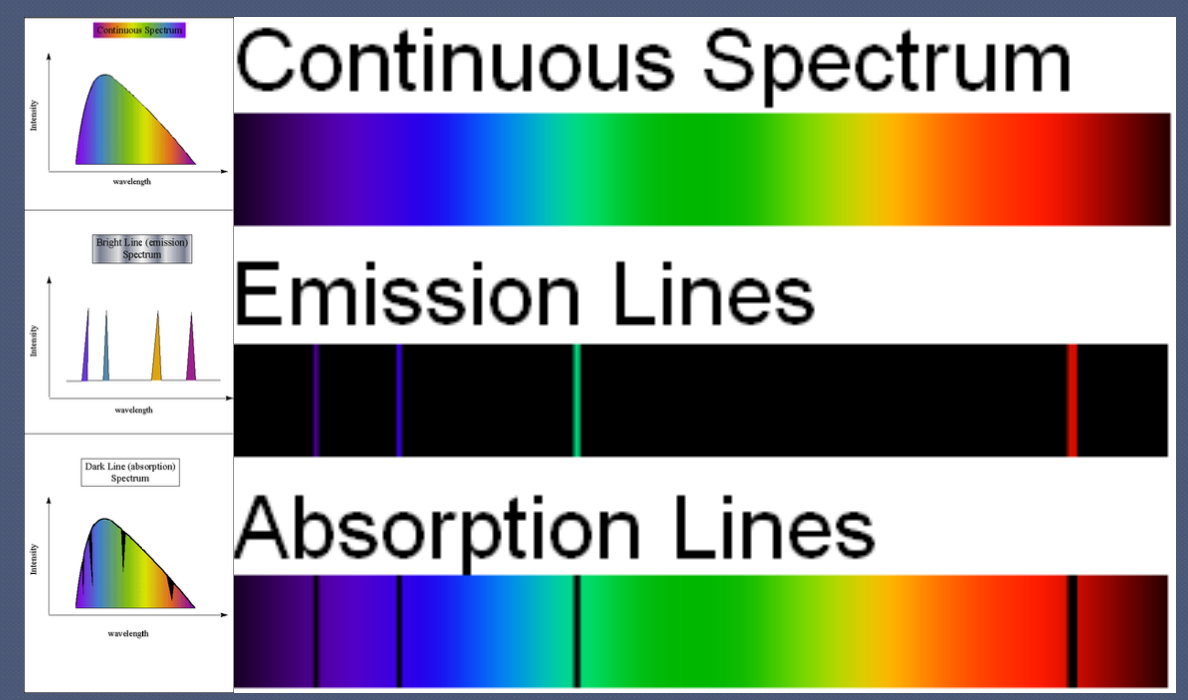
\includegraphics[width=12cm]{figures/figure1_4.png}
\captionsetup{justification=raggedright, singlelinecheck=false}
\caption{三种光谱。}
\label{三种光谱。}
\end{figure}

\subsubsection{热辐射和脉泽}
辐射机制可分为热辐射与非热辐射两类。热辐射本质是微观粒子热运动能量通过电磁相互作用的量子化释放,其宏观表现(如光谱分布)由统计物理与量子理论共同描述。一般来讲温度大于$0\,\mathrm{K}$的物质都能释放热辐射,同时这些物质也能吸收热辐射。大部分天体可见光波段辐射具有热辐射的性质。

一种特殊的热辐射是黑体辐射。黑体是一种能吸收所有波长电磁波的理想模型,其辐射仅由温度决定。当物质处于热动平衡状态(系统宏观性质如温度压强等不随时间变化,吸收与发射辐射平衡)时,热辐射具有黑体辐射的特征:其发射与吸收单色辐射能力的比值等于同温度下黑体发射单色辐射的能力,即
\begin{equation}
S_{\nu}=B_{\nu}\left(T\right).
\end{equation}
前文曾提到过,对于光学厚的介质我们所观测到的就是它的源函数,因此恒星具有黑体辐射特征。

我们将对此作进一步说明。首先,在热平衡状态下,两个能级的粒子数分布满足玻尔兹曼公式:
\begin{equation}
\frac{N_{r,k}}{N_{r,i}}=\frac{g_{r,k}}{g_{r,i}}\mathrm{e}^{-\frac{\varepsilon_{r,k}-\varepsilon_{r,i}}{k_{\text{B}}T}},\label{1.2.2}
\end{equation}
$r$表示该原子已经被电离了$r$个电子,表征电离级;$k,i$是第$r+1$个电子所处的能级,表征激发态,基态时$k=1$, $g$是统计权重;$\varepsilon$是从基态电离到该能级所需要的能量;$k_{\text{B}}$是玻尔兹曼常数。根据上式,热平衡状态时高能级原子数小于低能级原子数。但如果有某种外界能量输入使高能级原子数大于低能级原子数(称其为布居反转 (population invertion)),那么此时体系的“温度”小于$0$,称作负温度。负温度只是形式上的温度,此时系统并不处于热平衡状态。

根据 (\ref{1.2.2}) 式,同一电离级原子总数为
\begin{equation}
N_{r}=\sum_{i}N_{r,i}=\frac{N_{r,1}}{g_{r,1}}\left(g_{r,1}\mathrm{e}^{-\frac{\varepsilon_{r,1}-\varepsilon_{r,1}}{k_{\text{B}}T}}+g_{r,2}\mathrm{e}^{-\frac{\varepsilon_{r,2}-\varepsilon_{r,1}}{k_{\text{B}}T}}+\cdots\right)=\frac{N_{r,1}}{g_{r,1}}\left(g_{r,1}+g_{r,2}\mathrm{e}^{-\frac{\varepsilon_{r,2}}{k_{\text{B}}T}}+\cdots\right).
\end{equation}
定义配分函数
\begin{equation}
U_r(T)=\sum_{i=1}^\infty g_{r,i}\mathrm{e}^{-\frac{\varepsilon_{r,i}}{k_{\text{B}}T}},
\end{equation}
可以得到
\begin{equation}
N_{r}=\frac{N_{r,1}}{g_{r,1}}U_r(T)=\frac{N_{r,k}}{g_{r,k}}\mathrm{e}^{\frac{\varepsilon_{r,k}}{k_{\text{B}}T}}U_r(T).
\end{equation}

有一些机制可以引起原子在两能级间的跃迁。首先,处于高能级的原子本身就是不稳定的,会自发向低能级跃迁。在没有外辐射场的情况下,单位时间内一个原子从高能级$k$跃迁到低能级$i$同时在$\mathrm{d}\Omega$立体角内发射光子的概率为$A_{ki}\dfrac{\mathrm{d}\Omega}{4\pi}$.当辐射场存在时,高能级原子会受到扰动,向低能级跃迁并发出光子,该光子与辐射场入射光子在频率、相位、偏振、传播方向可能都相同。记单位时间由于受激辐射而产生的跃迁概率为$B_{ki}I_{\nu}\dfrac{\mathrm{d}\Omega}{4\pi}$.以后,低能级原子可以吸收辐射场光子能量跃迁到高能级,记受激吸收系数为$B_{ik}$.

因此单位时间内,$\mathrm{d}\Omega$内发射光子数目为
\begin{equation}
n_{k\to i}=N_k(A_{ki}+B_{ki}I_\nu)\frac{\mathrm{d}\Omega}{4\pi}.
\end{equation}
吸收光子数目为
\begin{equation}
n_{i\to k}=N_iB_{ik}I_\nu\frac{\mathrm{d}\Omega}{4\pi},
\end{equation}
热动平衡下存在细致平衡原理,即
\begin{equation}
N_k(A_{ki}+B_{ki}I_\nu)=N_iB_{ik}I_\nu.
\end{equation}
同时粒子数分布满足玻尔兹曼公式,得到
\begin{align}
A_{ki}+B_{ki}I_\nu&=\frac{g_i}{g_k}\mathrm{e}^{-\frac{\varepsilon_i-\varepsilon_k}{k_{\text{B}}T}}B_{ik}I_\nu,\\
I_\nu&=\frac{\frac{A_{ki}}{B_{ki}}}{\frac{g_iB_{ik}}{g_kB_{ki}}\mathrm{e}^\frac{h\nu_{ki}}{k_{\text{B}}T}-1}.
\end{align}
前文提到热动平衡下辐射强度等于$B_\nu(T)$,对比形式得到
\begin{align}
g_iB_{ik}&=g_kB_{ki},\\
A_{ki}&=\frac{2h\nu_{ki}^3}{c^2}B_{ki}.
\end{align}

因为受激发射和受激吸收都涉及到辐射场,一般将二者合在一起考虑。如图\ref{三种光谱。}所示,线谱一般并非一条无限细的线,而是有一定的轮廓。定义自发发射轮廓$\psi_\nu$,受激吸收和受激发射轮廓$\varphi_\nu$.物质发射系数可记作
\begin{equation}
j_\nu=\frac{h\nu}{4\pi}A_{ki}N_k\psi_\nu,
\end{equation}
吸收系数为
\begin{equation}
\alpha_{\nu}=\frac{h\nu}{4\pi}(B_{ik}N_i-B_{ki}N_{k})\varphi_\nu.\label{1.2.14}
\end{equation}
源函数
\begin{equation}
S_\nu=\frac{j_\nu}{\alpha_\nu}=\frac{A_{ki}}{B_{ki}}\frac{1}{\frac{g_k}{g_i}\frac{N_i}{N_k}-1}\frac{\psi_\nu}{\varphi
_\nu}=\frac{2h\nu^3}{c^2}\frac{1}{\frac{g_k}{g_i}\frac{N_i}{N_k}-1}\frac{\psi_\nu}{\varphi
_\nu}.
\end{equation}
即当$\psi_\nu=\varphi_\nu$,且原子分布满足玻尔兹曼分布时,源函数才转化为普朗克函数。

值得一提的是,此时吸收系数可以写作
\begin{equation}
\alpha_{\nu}=\frac{h\nu}{4\pi}B_{ik}N_{i}\left(1-\mathrm{e}^{-\frac{\varepsilon_{i}-\varepsilon_{k}}{k_{\text{B}}T}}\right)\varphi_{\nu}.
\end{equation}
如果$h\nu\ll k_{\text{B}}T$,且沿光线传播路径温度不变,那么光深
\begin{equation}
\tau_{\nu}=\int\alpha_{\nu}\mathrm{d}l\propto{}\int\frac{N_{i}\mathrm{d}l}{T},
\end{equation}
因此光深和温度和数密度有关。

一般情况下原子数目按能级分布会偏离玻尔兹曼分布:
\begin{align}
\frac{N_k}{N_i}&=\frac{b_k}{b_i}\frac{g_k}{g_i}\mathrm{e}^{-\frac{\varepsilon_i-\varepsilon_k}{k_{\text{B}}T}},\\
S_\nu&=\frac{2h\nu^3}{c^2}\frac{1}{\frac{b_i}{b_k}\mathrm{e}^{\frac{h\nu}{k_{\text{B}}T}}-1}\frac{\psi_\nu}{\varphi_\nu}.
\end{align}

观察 ($\ref{1.2.14}$) 式发现,如果$B_{ik}N_{i}<B_{ki}N_{k}$,那么吸收系数为负,相当于辐射沿着路径不断增强。此时高能级粒子跃迁到低能级时,释放的辐射被邻近粒子吸收,邻近粒子受激辐射,短时间内连续发生向低能级迁移,整体将形成强有力的放射。当放射波长为可见光到红外波段时称为激光 (Laser),射电的情形则称为微波受激辐射放大 (Microwave Amplification by Stimulated Emission of Radiation, Maser),又称脉泽。

为进一步研究脉泽,我们首先写出辐射转移方程:
\begin{equation}
\frac{\mathrm{d}I_{\nu}}{\mathrm{d}l}=-\frac{h\nu}{4\pi}\left(B_{ik}N_{i}-B_{ki}N_{k}\right)\varphi_{\nu}I_{\nu}+\frac{h\nu}{4\pi}N_{k}A_{ki}\psi_{\nu}.
\end{equation}
简单起见,不考虑谱线轮廓,并假设$B_{ik}=B_{ki}=4\pi B$,记$A=\dfrac{A_{ki}}{4\pi}$,则
\begin{equation}
\frac{\mathrm{d}I_{\nu}}{\mathrm{d}l}=-h\nu B\left(N_{i}-N_{k}\right)I_{\nu}+h\nu N_{k}A.
\end{equation}
接下来就要考虑两个能级间具体的粒子数关系建立完整的辐射转移方程。首先,Maser 是由分子(如水、羟基、甲醇等)能级跃迁产生的,而对于分子谱线来讲,$A_{ki}$可以忽略,因此等号右边第二项可以忽略。其次,尽管脉泽不是非热辐射无法用玻尔兹曼方程,但还是可以利用细致平衡原理。设外界能量输入引起的从下能级到上能级的粒子数抽运速度为$R$,两能级间的碰撞跃迁速率为$C$,则有
\begin{equation}
N_{i}\left(BI_{\nu}+C\right)+R=N_{k}\left(BI_{\nu}+C\right),
\end{equation}
因此
\begin{align}
N_{k}-N_{i}&=\frac{R}{BI_{\nu}+C}.\\
\frac{\mathrm{d}I_{\nu}}{\mathrm{d}l}&=h\nu \frac{BRI_{\nu}}{BI_{\nu}+C}.
\end{align}
可见$C\gg BI_{\nu}$时,$I=I_{0}\mathrm{e}^{\alpha l},\alpha=\dfrac{h\nu BR}{C}$,辐射强度随路径指数增长,称其为非饱和脉泽。$C\ll BI_{\nu}$时,$I_{\nu}=h\nu Rl$,随路径长度$l$线性增长,称为饱和脉泽。

Maser 强度极高,比热辐射的高几个数量级,易与其他辐射区分。由于其强度极高,且不像可见光那样容易被尘埃散射,可以利用脉泽进行三角视差测距,可以确定银河系旋臂结构,测量星系距离,校准宇宙膨胀速率。前文提到有外界能量输入时,可以实现布居反转。外界能量可以来自恒星形成区(新生恒星周围的高密度气体云被激发),红巨星和超巨星包层(恒星喷发物质中的分子在膨胀气体中受激辐射)以及活动星系核(星系中心超大质量黑洞周围的吸积盘或喷流)。因此利用 Maser 的分布可以分析外界能量来源,研究星际空间动力学结构。Maser 信号有偏振特性,而左旋和右旋圆偏振波在有静磁场存在的等离子体中的折射率不同,因此传播速度不同,会发生偏振面旋转,因此 Maser 还可以反映天体磁场的分布。

\subsubsection{恒星的热辐射}
恒星是由炽热等离子体组成的,处于局域(光子自由程范围内)热动平衡,其粒子的运动遵循 Maxwell-Boltzman 分布,可以用“温度”来标记其平衡态,可看作是黑体辐射。局域热动意味着不同区域温度不一样,无法用一个统一的黑体谱来描述,传达到恒星表面的光,是恒星内部各组分黑体谱的贡献,故需要解辐射从恒星内部传播到表面的转移方程。首先,假定恒星球坐标下对称,黑体谱只和半径有关,$S_{\nu}=B_{\nu}\left(r\right)$.

\begin{figure}[!htp]
\centering
\tikzset{every picture/.style={line width=0.75pt}}
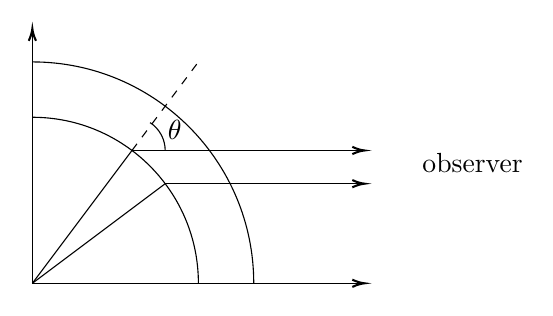
\begin{tikzpicture}[x = 0.4pt, y = 0.4pt, yscale = 1, xscale = 1]
\draw (0, 0) -- (0, 230);
\draw [shift = {(0, 230)}, rotate = 270][line width = 0.75] (10.93, -3.29) .. controls (6.95, -1.4) and (3.31, -0.3) .. (0, 0) .. controls (3.31, 0.3) and (6.95, 1.4) .. (10.93, 3.29);
\draw (0, 0) -- (300, 0);
\draw [shift = {(300, 0)}, rotate = 180][line width = 0.75](10.93, -3.29) .. controls (6.95, -1.4) and (3.31, -0.3) .. (0, 0) .. controls (3.31, 0.3) and (6.95, 1.4) .. (10.93, 3.29);
\draw (200, 0) arc (0:90:200);
\draw (150, 0) arc (0:90:150);
\draw (0, 0) -- (90, 120);
\draw [dashed](90, 120) -- (150, 200);
\draw (90, 120) -- (300, 120);
\draw [shift = {(300, 120)}, rotate = 180][line width = 0.75](10.93, -3.29) .. controls (6.95, -1.4) and (3.31, -0.3) .. (0, 0) .. controls (3.31, 0.3) and (6.95, 1.4) .. (10.93, 3.29);
\draw (120, 120) arc (0:57:30);
\draw (120, 150) node [anchor = north west][inner sep = 0.75pt][align = left] {$\theta$};
\draw (350, 120) node [anchor = north west][inner sep = 0.75pt][align = left] {observer};
\draw (0, 0) -- (120, 90);
\draw (120, 90) -- (300, 90);
\draw [shift = {(300, 90)}, rotate = 180][line width = 0.75](10.93, -3.29) .. controls (6.95, -1.4) and (3.31, -0.3) .. (0, 0) .. controls (3.31, 0.3) and (6.95, 1.4) .. (10.93, 3.29);
\end{tikzpicture}
\captionsetup{justification=raggedright, singlelinecheck=false}
\caption{恒星相同半径处不同位置光传播示意图。}
\label{恒星相同半径处不同位置光传播示意图。}
\end{figure}

其次,如图\ref{恒星相同半径处不同位置光传播示意图。}所示,相同半径处,$\theta$不同,所经历的消光是不一样的。我们观测到的太阳圆面,靠近中心处$\theta\to0$,穿过的大气较少,消光弱,圆面边缘处消光就强。(基于相同的原因,实际天文观测要观测天顶附近的恒星,因为此时光通过的地球大气较少。)光实际走过的距离$\mathrm{d}l$满足$\mathrm{d}l\cos\theta=\mathrm{d}r$,因此辐射转移方程可以写作
\begin{equation}
\frac{\mathrm{d}I_{\nu}}{\mathrm{d}r}\cos\theta=j_{\nu}-\alpha_{\nu}I_{\nu}.
\end{equation}
因为粒子分布也是各向同性的,故$\alpha_{\nu}$也只和$r$有关。尽管实际走过的光深为$\alpha_{\nu}\left(r\right)\mathrm{d}r\sec\theta$,但为了保留$\theta$的独立性,也为了建立光深和半径的对应关系,定义$\mathrm{d}\tau_{\nu}\left(r\right)=\alpha_{\nu}\left(r\right)\mathrm{d}r$,辐射转移方程写作
\begin{equation}
\cos\theta\frac{\mathrm{d}I_{\nu}\left(\theta,r\right)}{\mathrm{d}\tau_{\nu}\left(r\right)}=S_{\nu}\left(r\right)-I_{\nu}\left(\theta,r\right).
\end{equation}
每一项都是$r$的函数,也就意味着每一项都是光深的函数,而我们对后者更感兴趣,因此方程写作
\begin{equation}
\cos\theta\frac{\mathrm{d}I_{\nu}\left(\theta,\tau_{\nu}\right)}{\mathrm{d}\tau_{\nu}}=S_{\nu}\left(\tau_{\nu}\right)-I_{\nu}\left(\theta,\tau_{\nu}\right).
\end{equation}
尽管我们还不知道$S_{\nu}$对$\tau_{\nu}$的依赖关系,但我们可以给出上述方程的形式解。

首先,每个体元都有向外和向内(指向恒星内部)辐射的部分
\begin{equation}
I_\nu=\begin{cases}
I_\nu(\theta,\tau_\nu), & 0\le\theta<\frac{\pi}{2},\\
I_\nu'(\psi,\tau_\nu), & \frac{\pi}2<\theta\le\pi,\psi=\pi-\theta.
\end{cases}
\end{equation}
一般的辐射转移教材中,$\mathrm{d}r$是从恒星表面向下计量的,因此方程要变号。向外的辐射转移方程为
\begin{equation}
\cos\theta\frac{\mathrm{d}I_\nu(\theta,\tau_\nu)}{\mathrm{d}\tau_\nu}=I_\nu(\theta,\tau_\nu)-S_\nu(\tau_\nu),
\end{equation}
向内
\begin{equation}
-\cos\psi\frac{\mathrm{d}I'_\nu(\psi,\tau_\nu)}{\mathrm{d}\tau_\nu}=I'_\nu(\psi,\tau_\nu)-S_\nu(\tau_\nu).
\end{equation}
解得
\begin{align}
I_\nu(\theta,\tau_\nu)&=C_\nu\mathrm{e}^{\tau_\nu\sec\theta}+\mathrm{e}^{\tau_\nu\sec\theta}\int_{\tau_\nu}^\infty S_\nu(t_\nu)\mathrm{e}^{-t_\nu\sec\theta}\sec\theta\mathrm{d}t_\nu,\\
I'_\nu(\psi,\tau_\nu)&=D_\nu\mathrm{e}^{-\tau_\nu\sec\psi}+\mathrm{e}^{-\tau_\nu\sec\psi}\int_{0}^{\tau_\nu} S_\nu(t_\nu)\mathrm{e}^{t_\nu\sec\psi}\sec\psi\mathrm{d}t_\nu.
\end{align}
可以发现得到的形式解与前文形式类似,只是角度独立出来。

接着分析边界条件。恒星表面物质密度为零,光深肯定为零,同时从外向内的辐射也为零,因此$D=0$.在恒星最中心,是炽热的热核反应区域,可认为那里的光几乎传不到恒星表面,$\tau_{\nu}=\infty$,但是辐射强度依然是有限值,因此$C=0$.简化后的形式解为
\begin{align}
I_\nu(\theta,\tau_\nu)&=\int_{\tau_\nu}^{\infty}S_\nu(t_\nu)\mathrm{e}^{-(t_\nu-\tau_\nu) \sec\theta}\sec\theta\mathrm{d}t_\nu,\\
I_\nu'(\psi,\tau_\nu)&=\int_0^{\tau_\nu}S_\nu(t_\nu)\mathrm{e}^{-(\tau_\nu-t_\nu)\sec\psi}\sec\psi\mathrm{d}t_\nu.
\end{align}
积分限代表对辐射强度有贡献的区域,积分内$\mathrm{e}$​的负指数代表消光的影响。实际观测量为(如果沿途没有消光的话)
\begin{equation}
I_\nu(\theta,0)=\int_{0}^{\infty}S_\nu(t_\nu)\mathrm{e}^{-t_\nu\sec\theta}\sec\theta\mathrm{d}t_\nu,
\end{equation}

要使形式解真正有用,我们需要寻找源函数与光学深度的联系。假设呈现某种线性关系(或看作源函数泰勒展开一阶近似)
\begin{equation}
S_{\nu}\left(t_{\nu}\right)=S_{0}+S_{1}t_{\nu},
\end{equation}
积分结果为
\begin{equation}
I_\nu(\theta,0)=S_{0}+S_{1}\cos\theta.
\end{equation}
观察这个结果我们发现,观测量实际上为$\tau_{\nu}=\cos\theta$处的源函数。而光实际上走过的光深为$\tau_{\nu}\sec\theta$,因此我们所见的恒星其实是光深为$1$处的恒星。也正因如此,光深为$1$在天文研究中是个有意义的参量。我们所见到的天体的“表面”都可以看作是光深为$1$处的表面。

值得注意的是,恒星不同元素含量不同,原子能级结构也不同,因此对不同的单色辐射来讲,相同半径处$\alpha_{\nu}$也不同。换句话讲,即使光深都为$1$,随频率变化所对应的半径也是不同的,因此恒星圆面一小部分区域的黑体谱也是不同半径处黑体谱的拼接。可能在 B 波段所“采用”的是$r_{1}$的一段黑体谱,在 V 波段是$r_{2}$处的一段黑体谱。因此“恒星光谱近似黑体光谱”还有这层含义。在不同滤光片中所见到的恒星可如图\ref{不同波段所见到的光深为 1 处的恒星。}蓝色和红色线条所示。不过实际多半不会这么圆滑,取决于$\alpha_{\nu}$和半径的具体关系。

\begin{figure}[!htp]
\centering
\tikzset{every picture/.style={line width=0.75pt}}
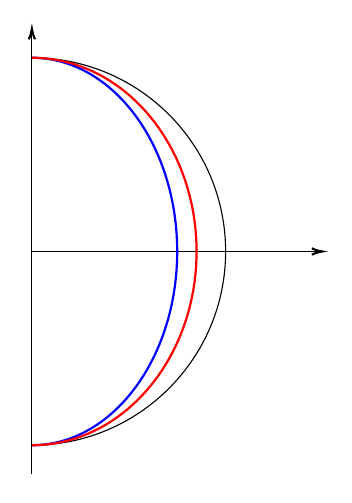
\begin{tikzpicture}[x = 0.35pt, y = 0.35pt, yscale = 1, xscale = 1]
\draw (0, -230) -- (0, 230);
\draw [shift = {(0, 230)}, rotate = 270][line width = 0.75] (10.93, -3.29) .. controls (6.95, -1.4) and (3.31, -0.3) .. (0, 0) .. controls (3.31, 0.3) and (6.95, 1.4) .. (10.93, 3.29);
\draw (0, 0) -- (300, 0);
\draw [shift = {(300, 0)}, rotate = 180][line width = 0.75](10.93, -3.29) .. controls (6.95, -1.4) and (3.31, -0.3) .. (0, 0) .. controls (3.31, 0.3) and (6.95, 1.4) .. (10.93, 3.29);
\draw (200, 0) arc (0:90:200);
\draw (200, 0) arc (0:-90:200);
\draw [blue, thick](150, 0) arc (0:90:150 and 200);
\draw [blue, thick](150, 0) arc (0:-90:150 and 200);
\draw [red, thick](170, 0) arc (0:90:170 and 200);
\draw [red, thick](170, 0) arc (0:-90:170 and 200);
\end{tikzpicture}
\captionsetup{justification=raggedright, singlelinecheck=false}
\caption{不同波段所见到的光深为 1 处的恒星。}
\label{不同波段所见到的光深为 1 处的恒星。}
\end{figure}

\subsubsection{高斯单位制}
国际单位制 (SI) 中,与力学和电磁学有关的基本单位有$\mathrm{kg,m,s,A}$.之所以选择$\mathrm{A}$而不是电荷是因为电流比较好测定。$\mathrm{A}$的定义方式如下:考虑$F=\dfrac{\mu_{0}I_{1}I_{2}L}{2\pi r}$,两根电流相同的直导线,相距$r=1\,\mathrm{m}$的情况下,单位长度产生$2\times10^{-7}\,\mathrm{N}$的相互作用力时,导线中通过的电流强度为$1\,\mathrm{A}$.此定义等价于定义真空磁导率为$\mu_{0}=4\pi\times10^{-7}\,\mathrm{kg\cdot m\cdot A^{-2}\cdot s^{-2}}$.另外可得电荷单位$1\,\mathrm{C}=\sqrt{4\pi\varepsilon_{0}}\cdot\mathrm{N^{\frac12}\cdot m}$.

而在厘米克秒制 (cgs) 中,只有$\mathrm{g,cm,s}$三个基本单位。首先导出力的单位$1\,\mathrm{dyne}=1\,\mathrm{g\cdot cm\cdot{}s^{-2}}=10^{-5}\,\mathrm{N}$以及能量单位$1\,\mathrm{erg}=1\,\mathrm{g\cdot cm^{2}\cdot{}s^{-2}}=10^{-7}\,\mathrm{J}$.

静电制中力与电磁的桥梁是库仑定律$F=\dfrac{1}{4\pi\varepsilon_{0}}\dfrac{q_{1}q_{2}}{r^{2}}$.静电制不希望看到前面的系数,故选择定义真空介电常数,取$\varepsilon_{0\text{cgs}}=\dfrac{1}{4\pi},\mu_{0\text{cgs}}=\dfrac{4\pi}{c^{2}}$,其中$c$为真空光速。换句话讲静电制定义了$1\,\mathrm{A}=0.1c\cdot\mathrm{dyne}^{\frac12},1\,\mathrm{C}=0.1c\cdot\rm{dyne}^{\frac12}\cdot s$.类似的操作可在自然单位制中见到,那里定义$1\,\mathrm{s}=3\times10^{8}\,\mathrm{m}$故$c=1$.

不管怎样库仑定律简化为$F=\dfrac{q_{1}q_{2}}{r^{2}}$,静电制中电荷单位也变为$1\,\mathrm{statC}=1\,\mathrm{dyne^{\frac12}\cdot cm}$.考虑无量纲的真空光速数值$c_{n},1\,\mathrm{C}=2.99792458\times10^{9}\,\mathrm{statC}$.静电制中电流基本单位$1\,\mathrm{statA}=1\,\mathrm{esu}=1\,\mathrm{statC\cdot{}s^{-1}}$.考虑$B=\dfrac{F}{IL}$我们还可以得到磁感应强度基本单位$1\,\mathrm{statT}=1\,\mathrm{dyne^{\frac{1}{2}}\cdot cm^{-2}\cdot s}=10^{-4}c_{n}\mathrm{T}$.

而在静磁制中,电流的基本单位用以下方法定义:相距$1\,\mathrm{cm}$单位长度产生$2\,\mathrm{dyne}$相互作用力时的导线中的电流强度为$1\,\mathrm{emu}$.即$1\,\mathrm{emu}=c\cdot\rm dyne^{\frac12}=10\,\mathrm{A}$.此时得到静磁制下磁感应强度基本单位$1\,\mathrm{G}=\dfrac{1}{c}\cdot\mathrm{dyne}^{\frac12}\cdot\mathrm{cm}^{-1}=10^{-4}\,\mathrm{T}=\dfrac1{c_{n}}\,\mathrm{statT}$.

高斯单位制杂糅了静电制和静磁制,在电荷上使用静电制,磁场上使用静磁制,数值运算的时候可能会出现问题。如进行运动学运算的时候不能简单使用如$B=3\,\mu\mathrm{G}$的数据,而要转变成$B=\dfrac{3\mu}{c_{n}}\,\mathrm{statT}$进行运算,否则静电制和静磁制会相互冲突。

但有意思的是,相对一般的 cgs 制,高斯单位制还有一个独立选择,定义$B_{\text{G}}=c\cdot B_{\text{cgs}}$,使电场强度和磁感应强度有相同的量纲。这时候有些公式会变形,如洛伦兹力公式会变为$\boldsymbol{F}=q\dfrac{\boldsymbol{v}}c\times\boldsymbol{B}_{\text{G}}$.考虑数值计算我们会惊奇地发现$B_{\text{G}}=3\,\mu\dfrac{c}{c_{n}}\,\mathrm{statT}=3\,\mu\cdot\mathrm{statT}\cdot\mathrm{cm\cdot{}s^{-1}}=3\,\mu\,\mathrm{dyne^{\frac{1}{2}}}\cdot\mathrm{cm}^{-1}$.即本质上$B_{\text{cgs}}=n\,\mathrm{G}$,运算上$B_{\text{G}}=n\,\mathrm{dyne^{\frac{1}{2}}\cdot cm^{-1}}$,高斯单位制成功统一了数值和量纲。

\subsubsection{运动粒子的辐射}
接下来要讲的是非热辐射。非热辐射能谱一般和热辐射很不一样,后者特征是黑体谱,而一些重要的非热辐射为幂律谱,即辐射强度与频率的指数成正比。原因在于二者机制不同。热辐射来自能级跃迁产生的辐射,非热辐射主要来自运动的带电粒子。查询一般电动力学教程可知,运动带电粒子的电磁场为
\begin{equation}
\boldsymbol{E}\left(x,y,z,t\right)=q\left[\frac{\left(\boldsymbol{n}-\boldsymbol{\beta}\right)\left(1-\boldsymbol{\beta}^{2}\right)}{K^{3}r^{2}}\right]_{\text{ret}}+\frac{q}{c}\left\{\frac{\boldsymbol{n}}{K^{3}r}\times\left[\left(\boldsymbol{n}-\boldsymbol{\beta}\right)\times\dot{\boldsymbol{\beta}}\right]\right\}_{\text{ret}}.\label{1.3.38}
\end{equation}
其中 ret 表示 retarded potentials,推迟势,即因为光速有限,时刻$t$观测者观测到的电磁场是时刻$t'$粒子所在处的电磁场。$\boldsymbol{n}$是$t'$时刻粒子所在处到观测者方向的单位矢量,$\boldsymbol{\beta}=\dfrac{\boldsymbol{v}}{c},K=1-\boldsymbol{n}\cdot\boldsymbol{\beta},\boldsymbol{v}$是粒子速度。等号右侧第一项在粒子静止时退化为库仑场,第二项是辐射场,在粒子作加速运动时才产生。有不少机制能让粒子获得能量进行运动,产生非热辐射,比如回旋辐射(电子在磁场中非相对论性螺旋运动)、同步加速辐射(电子在磁场中相对论性螺旋运动)、曲率辐射(电子在弯曲磁力线中运动)、逆康普顿散射(电子与光子碰撞,能量转移给光子)、轫致辐射(带电粒子碰撞,电子受库仑场影响骤然减速,又称刹车辐射、自由{}-{}自由跃迁)、切伦科夫辐射(即使不作加速运动,粒子速度超过介质光的相速度时也会产生辐射)。注意到主要涉及电子与电磁场的作用。这是为什么呢?而电子作为带电粒子,质量相比其他粒子极小,容易被加速,且能被加速到相对论速度,因此它产生的辐射最强。

讨论辐射问题时,我们总会关心粒子在单位时间中辐射的能量(功率),不同方向的辐射强度(角分布),不同频率的辐射强度(谱分布)以及辐射的偏振情况。

我们先来研究角分布。我们用 Poynting 矢量描述空间中某一点的瞬时能量通量:
\begin{equation}
\boldsymbol{S}=\frac{1}{\mu_{0}}\boldsymbol{E}\times\boldsymbol{B}_{\text{SI}}=\frac{c^{2}}{4\pi}\boldsymbol{E}\times\frac{\boldsymbol{B}_{\text{G}}}{c}=\frac{c}{4\pi}\boldsymbol{E}\times\left(\boldsymbol{n}\times\boldsymbol{E}\right)=\frac{c}{4\pi}\left\vert{}\boldsymbol{E}\right\vert{}^{2}\boldsymbol{n}.
\end{equation}
在观察点$\left(x,y,z\right)$作一小面元$\mathrm{d}\boldsymbol{\sigma}$,其法向沿 Poynting 矢量方向。该面元对$t'$时刻粒子所在点张的立体角为$\mathrm{d}\Omega,\mathrm{d}\boldsymbol{\sigma}=r^{2}\mathrm{d}\Omega\boldsymbol{n}$,故单位时间通过$\mathrm{d}\boldsymbol{\sigma}$的能量为
\begin{equation}
\mathrm{d}P\left(t\right)=\boldsymbol{S}\cdot\mathrm{d}\boldsymbol{\sigma}=\left(\boldsymbol{S}\cdot\boldsymbol{n}\right)r^{2}\mathrm{d}\Omega=\frac{c}{4\pi}r^{2}\left\vert{}\boldsymbol{E}\right\vert{}^{2}\mathrm{d}\Omega.
\end{equation}
由此我们就得到了每单位立体角辐射的功率。但需要注意的是,这是$t'$时刻发出的辐射$t$时刻的观测者处所接收到的部分,而我们更关心$t'$时刻粒子处的辐射分布。所以需要改写。$t\text{\textendash}t+\mathrm{d}t$时间段内观测者在面元$\mathrm{d}\sigma$中接收的能量$\mathrm{d}P\left(t\right)\mathrm{d}t$是电荷在$t'\text{\textendash}t'+\mathrm{d}t'$时间段内发出的,按能量守恒有
\begin{equation}
\mathrm{d}P\left(t'\right)=\mathrm{d}P\left(t\right)\frac{\mathrm{d}t}{\mathrm{d}t'}.
\end{equation}
已知
\begin{equation}
t'=t-\frac{r\left(t'\right)}{c},
\end{equation}
故
\begin{equation}
\mathrm{d}t'=\mathrm{d}t-\frac{1}{c}\frac{\mathrm{d}r\left(t'\right)}{\mathrm{d}t'}\mathrm{d}t'=\mathrm{d}t+\frac{1}{c}\boldsymbol{v}\left(t'\right)\cdot\boldsymbol{n}\mathrm{d}t',
\end{equation}
由此可见
\begin{equation}
\frac{\mathrm{d}t}{\mathrm{d}t'}=1-\boldsymbol{n}\cdot\boldsymbol{\beta}=K.
\end{equation}
因此粒子单位时间中沿给定方向单位立体角辐射的能量为
\begin{equation}
\frac{\mathrm{d}P\left(t'\right)}{\mathrm{d}\Omega}=\frac{\mathrm{d}P\left(t\right)}{\mathrm{d}\Omega}\frac{\mathrm{d}t}{\mathrm{d}t'}=\frac{cK}{4\pi}r^{2}\left\vert{}\boldsymbol{E}\right\vert{}^{2}.
\end{equation}
注意 (\ref{1.3.38}) 式等号右侧第二项,由此得出粒子辐射的角分布特征:
\begin{equation}
\frac{\mathrm{d}P\left(t'\right)}{\mathrm{d}\Omega}=\frac{q^{2}}{4\pi c}\frac{\left\{\boldsymbol{n}\times\left[\left(\boldsymbol{n}-\boldsymbol{\beta}\right)\times\dot{\boldsymbol{\beta}}\right]\right\}^{2}}{K^{5}}.\label{1.3.46}
\end{equation}

非相对论情形下,$\beta\to0,K\to1$,此时上式简化为
\begin{equation}
\frac{\mathrm{d}P\left(t'\right)}{\mathrm{d}\Omega}=\frac{q^{2}}{4\pi c}\left[\boldsymbol{n}\times\left(\boldsymbol{n}\times\dot{\boldsymbol{\beta}}\right)\right]^{2}.
\end{equation}
用$\theta$表示加速度$\dot{\boldsymbol{v}}$和$\boldsymbol{n}$的夹角,则有
\begin{equation}
\frac{\mathrm{d}P\left(t'\right)}{\mathrm{d}\Omega}=\frac{q^{2}\dot{\boldsymbol{v}}^{2}}{4\pi c^{3}}\sin^{2}\theta.
\end{equation}
实际上这是偶极辐射的角分布,$q^{2}\dot{\boldsymbol{v}}^{2}$就是偶极子$\boldsymbol{d}$的二阶时间导数。非相对论的辐射角分布有两个特点,其一辐射和速度无关而和加速度有关,其二辐射分布在很宽的角范围中。具体可如图\ref{非相对论性粒子辐射的角分布。}所示。
\begin{figure}[!htbp]
\centering
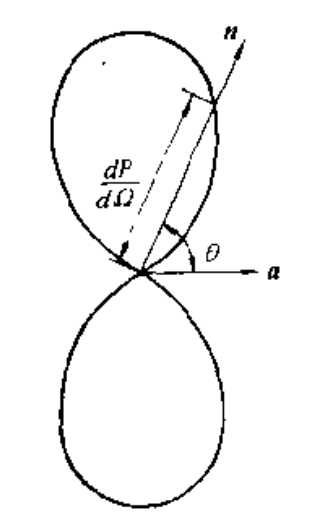
\includegraphics[width=3cm]{figures/figure1_5.png}
\captionsetup{justification=raggedright, singlelinecheck=false}
\caption{非相对论性粒子辐射的角分布。}
\label{非相对论性粒子辐射的角分布。}
\end{figure}

你好{}-{}你哈

而对相对论性粒子的辐射我们先来作一些定性分析。根据 (\ref{1.3.46}) 式不难看出相对论速度对角分布有所影响,因为分子含$\beta^{2}$项而分母含$\beta^{5}$项。由于$K=1-\boldsymbol{n}\cdot\boldsymbol{\beta}$,当$\beta\to1$时,如果$\boldsymbol{n}$指向$\boldsymbol{\beta}$的方向,$K\to0$,此时$\dfrac{\mathrm{d}P\left(t'\right)}{\mathrm{d}\Omega}\to\infty$,即辐射能量极大地集中在粒子运动的方向上,这被称作集束效应 (beaming effect).

进一步地,我们认为辐射集中以粒子运动方向为中心线,张角为$\theta=\dfrac{1}{\gamma}=\sqrt{1-\dfrac{v^{2}}{c^{2}}}=\sqrt{1-\beta^{2}}$的圆锥范围内。$\theta=\sqrt{1-\beta^{2}}$时认为此时$K$大约是极大值的$\dfrac{1}{2}$,辐射也相对极大方向下降到$\dfrac{1}{2^{5}}$.电子速度可以达到$\gamma\sim10^{6}$,对应$\theta\sim0.2^{\prime\prime}$,因此相对论性粒子辐射十分集中。

进一步,为了定量说明相对论粒子辐射角分布具体图形,考虑速度与加速度方向相互平行和相互垂直两种情况。先考虑平行情况,此时辐射角分布为
\begin{equation}
\frac{\mathrm{d}P\left(t'\right)}{\mathrm{d}\Omega}=\frac{q^{2}}{4\pi c}\frac{\dot{\beta}^{2}\sin^{2}\theta}{\left(1-\beta\cos\theta\right)^{5}},
\end{equation}
其中$\theta$是$\boldsymbol{n}$和速度方向的夹角。此时的角分布图形与非相对论情形的对比可如图\ref{加速度与速度平行时相对论性粒子的辐射角分布。}所示。
\begin{figure}[!htbp]
\centering
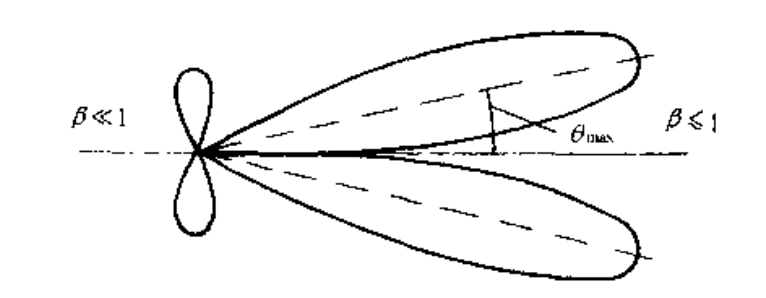
\includegraphics[width=9cm]{figures/figure1_6.png}
\captionsetup{justification=raggedright, singlelinecheck=false}
\caption{加速度与速度平行时相对论性粒子的辐射角分布。}
\label{加速度与速度平行时相对论性粒子的辐射角分布。}
\end{figure}

垂直情况则要稍微复杂一点。不过这种情形可能更加常见,因为粒子在磁场中运动受洛伦兹力影响加速度与速度往往是垂直的。注意矢量公式
\begin{equation}
\boldsymbol{A}\times\left(\boldsymbol{B}\times\boldsymbol{C}\right)=\boldsymbol{B}\left(\boldsymbol{A}\cdot\boldsymbol{C}\right)-\boldsymbol{C}\left(\boldsymbol{A}\cdot\boldsymbol{B}\right),
\end{equation}
可知
\begin{align}
\boldsymbol{n}\times\left[\left(\boldsymbol{n}-\boldsymbol{\beta}\right)\times\dot{\boldsymbol{\beta}}\right]&=\left(\boldsymbol{n}-\boldsymbol{\beta}\right)\left(\boldsymbol{n}\cdot\dot{\boldsymbol{\beta}}\right)-\dot{\boldsymbol{\beta}}\left[\boldsymbol{n}\cdot\left(\boldsymbol{n}-\boldsymbol{\beta}\right)\right]\notag\\
&=\left(\boldsymbol{n}\cdot\dot{\boldsymbol{\beta}}\right)\boldsymbol{n}-\left(\boldsymbol{n}\cdot\dot{\boldsymbol{\beta}}\right)\boldsymbol{\beta}-\left(1-\boldsymbol{n}\cdot\boldsymbol{\beta}\right)\dot{\boldsymbol{\beta}}.
\end{align}
注意$\boldsymbol{\beta}\cdot\dot{\boldsymbol{\beta}}=0$,因此平方后得到
\begin{align}
&\quad\,\left(1-\boldsymbol{n}\cdot\boldsymbol{\beta}\right)^{2}\dot{\boldsymbol{\beta}}^{2}+\left(1+\beta^{2}-2\boldsymbol{n}\cdot\boldsymbol{\beta}\right)\left(\boldsymbol{n}\cdot\dot{\boldsymbol{\beta}}\right)^{2}-2\left(1-\boldsymbol{n}\cdot\boldsymbol{\beta}\right)\dot{\boldsymbol{\beta}}\cdot\left(\boldsymbol{n}\cdot\dot{\boldsymbol{\beta}}\right)\left(\boldsymbol{n}-\boldsymbol{\beta}\right)\notag\\
&=\left(1-\boldsymbol{n}\cdot\boldsymbol{\beta}\right)^{2}\dot{\boldsymbol{\beta}}^{2}+\left(1+\beta^{2}-2\boldsymbol{n}\cdot\boldsymbol{\beta}\right)\left(\boldsymbol{n}\cdot\dot{\boldsymbol{\beta}}\right)^{2}-2\left(1-\boldsymbol{n}\cdot\boldsymbol{\beta}\right)\left(\boldsymbol{n}\cdot\dot{\boldsymbol{\beta}}\right)^{2}\notag\\
&=\left(1-\boldsymbol{n}\cdot\boldsymbol{\beta}\right)^{2}\dot{\boldsymbol{\beta}}^{2}+\left(-1+\beta^{2}\right)\left(\boldsymbol{n}\cdot\dot{\boldsymbol{\beta}}\right)^{2}.
\end{align}
因此辐射角分布公式为
\begin{equation}
\frac{\mathrm{d}P\left(t'\right)}{\mathrm{d}\Omega}=\frac{q^{2}}{4\pi c}\frac{\left(1-\boldsymbol{n}\cdot\boldsymbol{\beta}\right)^{2}\dot{\boldsymbol{\beta}}^{2}-\left(1-\beta^{2}\right)\left(\boldsymbol{n}\cdot\dot{\boldsymbol{\beta}}\right)^{2}}{\left(1-\boldsymbol{n}\cdot\boldsymbol{\beta}\right)^{5}}.
\end{equation}
以$\theta$表示$\boldsymbol{n}$与$\boldsymbol{\beta}$的夹角,$\varphi$表示$\boldsymbol{n}$与$\boldsymbol{\beta}$所成平面与$\dot{\boldsymbol{\beta}}$的夹角,并注意$\boldsymbol{n}\cdot\dot{\boldsymbol{\beta}}=\dot{\boldsymbol{\beta}}\cos\varphi\sin\theta$,有
\begin{equation}
\frac{\mathrm{d}P\left(t'\right)}{\mathrm{d}\Omega}=\frac{q^{2}}{4\pi c}\dot{\boldsymbol{\beta}}^{2}\frac{\gamma^{2}\left(1-\beta\cos\theta\right)^{2}-\sin^{2}\theta\cos^{2}\varphi}{\gamma^{2}\left(1-\beta\cos\theta\right)^{5}}.
\end{equation}
此时辐射角分布可如图\ref{加速度与速度垂直时相对论性粒子的辐射角分布。}所示。
\begin{figure}[!htbp]
\centering
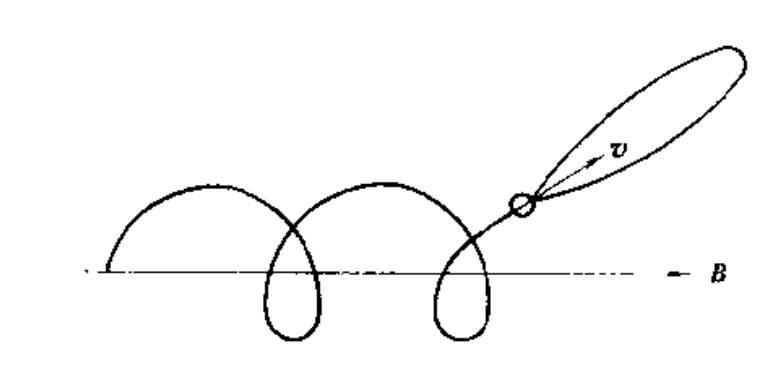
\includegraphics[width=8cm]{figures/figure1_7.png}
\captionsetup{justification=raggedright, singlelinecheck=false}
\caption{加速度与速度垂直时相对论性粒子的辐射角分布。}
\label{加速度与速度垂直时相对论性粒子的辐射角分布。}
\end{figure}

有了辐射的角分布公式,对所有方向的立体角积分就能得到辐射总功率。

对非相对论粒子,此时$\mathrm{d}\Omega=2\pi\sin\theta\mathrm{d}\theta$,得到总功率为
\begin{equation}
P\left(t'\right)=\frac{\mathrm{d}W}{\mathrm{d}t'}=\int\frac{q^{2}\dot{v}^{2}}{4\pi c^{3}}\sin^{2}\theta2\pi\sin\theta\mathrm{d}\theta=\frac{2q^{2}\dot{v}^{2}}{3c^{3}}.
\end{equation}
对相对论粒子,加速度与速度平行时
\begin{equation}
P_{\parallel}=\frac{2q^{2}}{3c}\gamma^{6}\dot{\beta}^{2}.
\end{equation}
垂直时
\begin{equation}
P_{\bot}=\frac{2q^{2}}{3c}\gamma^{4}\dot{\beta}^{2}.
\end{equation}
对于一般粒子的运动可以分解,进而得到
\begin{equation}
P=\frac{2q^{2}}{3c}\left(\gamma^{6}\dot{\beta}_{\parallel}^{2}+\gamma^{4}\dot{\beta}_{\bot}^{2}\right).
\end{equation}
也可以写成
\begin{equation}
P=\frac{2q^{2}}{3c}\gamma^{6}\left[\dot{\boldsymbol{\beta}}^{2}-\left(\boldsymbol{\beta}\times\dot{\boldsymbol{\beta}}\right)^{2}\right].\label{1.3.59}
\end{equation}

\subsubsection{同步加速辐射}
同步加速辐射可以说是最重要的非热辐射机制之一。星系中心的超大质量黑洞吸积物质时,强磁场在两极产生喷流 (jet),带电粒子在磁场中高速地加速运动,产生辐射,主要波段为射电波段,且辐射带有强烈的偏振特性。在图\ref{同步加速辐射示意图。}中,如果记磁场方向为$k$,考虑一个沿$k$轴运动的观测者,以他为参考系电子并非螺旋前进而是在一个平面上进行回旋运动,记这个平面为$ij$平面。因为集束效应,电子总会运动到这样一个状态,其辐射指向$j$方向,此时辐射可以分解为偏振方向互相垂直的两个部分,分别沿$i,k$方向,形成椭圆偏振光。可以证明在电子螺旋前进情形下,同步加速辐射依旧是椭圆偏振光。但由于推导过程过于复杂,本文不打算长篇大论。有关同步加速辐射的其他性质也将不加证明地给出。
\begin{figure}[!htbp]
\centering
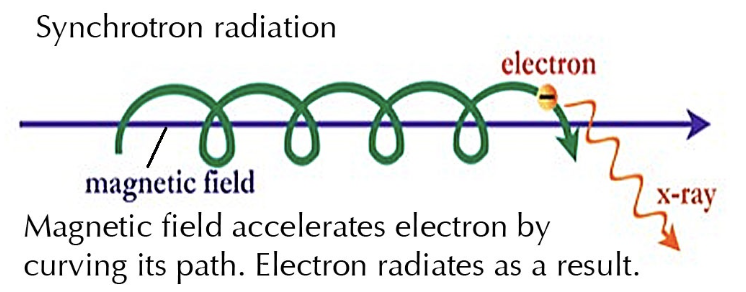
\includegraphics[width=8cm]{figures/figure1_8.png}
\captionsetup{justification=raggedright, singlelinecheck=false}
\caption{同步加速辐射示意图。}
\label{同步加速辐射示意图。}
\end{figure}

利用 (\ref{1.3.59}) 式,我们可以计算出单个电子在磁场中运动的辐射的功率:
\begin{equation}
P=\frac{2e^{4}}{3m_{0}^{2}c^{5}}\gamma^{2}v_{\bot}^{2}B^{2}.\label{1.3.60}
\end{equation}
其中$e$是电子电量,$B$是高斯单位制下的磁场强度,$m_{0}$是电子质量,$c$是光速。引入电子经典半径$r_{0}=\dfrac{e^{2}}{m_{0}c^{2}}$,上式写作
\begin{equation}
P=\frac{2}{3}r_{0}^{2}c\gamma^{2}\beta_{\bot}^{2}B^{2}.
\end{equation}
对于速度各向同性的电子集体,$\beta_{\bot}^{2}$对立体角平均后得到平均功率为
\begin{equation}
\langle{}P\rangle=\frac{4}{9}r_{0}^{2}c\gamma^{2}\beta^{2}B^{2}.
\end{equation}
引入汤姆孙散射截面$\sigma_{\text{T}}=\dfrac{8\pi}{3}r_{0}^{2}$和磁场能量密度$U_{B}=\dfrac{B^{2}}{8\pi}$,平均功率可以表示为
\begin{equation}
\langle{}P\rangle=\frac{4}{3}\sigma_{\text{T}}c\gamma^{2}\beta^{2}U_{B}.\label{1.2.35}
\end{equation}
对于 (\ref{1.3.60}) 式,我们发现$P=-\dfrac{\mathrm{d}E}{\mathrm{d}t}=bE^{2},b=\dfrac{2e^4}{3m_0^4c^9}B^{2}v_\bot^2$,解得,
\begin{equation}
E=\frac{E_0}{1+bE_0t}.
\end{equation}
电子能量下降到原先一半即$E=\dfrac12E_0$所用的时间(取$v_{\bot}=c$)为
\begin{align}
T_\frac12=\frac1{bE_0}&=\frac{3m_{0}^{3}c^{7}}{2e^{4}}\frac{1}{B^{2}v_\bot^2}\frac{m_0c^2}{E_0}\notag\\
&=\frac{5.1\times10^{8}\,\mathrm{s}}{B_{\text{数值}}^{2}}\frac{m_{0}c^{2}}{E_{0}}.
\end{align}

查阅《天体物理中的辐射机制》(尤峻汉)可知,同步加速辐射是一种连续谱,其单位频率间隔的辐射功率为
\begin{equation}
\langle\frac{\mathrm{d}P_\nu}{\mathrm{d}\nu}\rangle=\frac{\sqrt3e^3B}{m_0c^2}\frac{\nu}{\nu_c}\int_{\frac{\nu}{\nu_c}}^\infty K_\frac53(t)\mathrm{d}t,
\end{equation}
其中$K_{n}\left(x\right)$为$n$阶修正的贝塞尔函数。辐射功率在低频波段以$\nu^{\frac{1}{3}}$缓慢上升,辐射的峰值频率约为
\begin{equation}
\nu_{\max}=0.3\nu_{c}=\frac{9\gamma^2eB}{40\pi m_0c},
\end{equation}
峰值后辐射强度以自然常数的指数$\mathrm{e}^{-\frac{\nu}{\nu_{c}}}$快速下降。

上述结论适用于单个电子的辐射谱。而实际过程中肯定有很多电子在磁场中运动。对于数密度随能量分布为$E^{-\mu}$的电子集体,同步加速辐射谱满足
\begin{align}
\langle I_{\nu}\rangle&=\frac{2^{\frac{\mu-1}{2}}\sqrt3\Gamma(\frac{\mu+5}{4})\Gamma(\frac{3\mu-1}{12})\Gamma(\frac{3\mu+19}{12})}{8\sqrt\pi(\mu+1)\Gamma(\frac{\mu+7}{4})}\frac{e^{3}}{m_{0}c^{2}}(\frac{3e}{4\pi m_{0}^{3}c^{5}})^{\frac{\mu-1}2}B^{\frac{\mu+1}{2}}\nu^{-\frac{\mu-1}{2}}LN_{0}\notag\\
&=a(\mu)\frac{e^{3}}{m_{0}c^{2}}(\frac{3e}{4\pi m_{0}^{3}c^{5}})^{\frac{\mu-1}2}B^{\frac{\mu+1}{2}}\nu^{-\frac{\mu-1}{2}}LN_{0},\label{1.3.67}
\end{align}
其中$L$是沿视线方向辐射区域长度,$N_{0}$量纲$\mathrm{cm^{-3}\cdot erg^{\mu-1}}$,表征了数密度。根据上式可见辐射强度$\propto{}\nu^{-\frac{\mu-1}{2}}$,谱指数反映了电子能量分布。在典型 AGN 吸积活动中,$\mu=2.5$,可以发现辐射强度谱指数为$-0.75$.

对于电子集体来讲另一个要考虑的因素是,当电子密度足够大时,产生辐射的这些电子会与光子碰撞,反过来吸收辐射。吸收系数为
\begin{align}
\langle{}\alpha_{\nu}\rangle&=\frac{\sqrt{3}}{4}\Gamma\left(\frac{3\mu+2}{12}\right)\Gamma\left(\frac{3\mu+22}{12}\right)\frac{e^{3}}{2\pi m_{0}}\left(\frac{3e}{2\pi m_{0}^{3}c^{5}}\right)^{\frac{\mu}{2}}N_{0}\left(B\sin\alpha\right)^{\frac{\mu+2}{2}}\nu^{-\frac{\mu+4}{2}}\notag\\
&=g\left(\mu\right)\frac{e^{3}}{2\pi m_{0}}\left(\frac{3e}{2\pi m_{0}^{3}c^{5}}\right)^{\frac{\mu}{2}}N_{0}\left(B\sin\alpha\right)^{\frac{\mu+2}{2}}\nu^{-\frac{\mu+4}{2}}.\label{1.2.41}
\end{align}
可见低频波段吸收系数较大,相当于说低频波段电子相对辐射是光学厚的。我们知道光学厚观测到的辐射为源函数,将 (\ref{1.3.67})(\ref{1.2.41}) 式相比得到
\begin{equation}
S_{\nu}\propto{}\nu^{2.5}.
\end{equation}
因此低频波段的谱指数为$2.5$.

最后,同步加速辐射还有显著的偏振特征,单电子同步加速辐射为椭圆偏振光,偏振度为
\begin{equation}
\Pi=\frac{K_{\frac{2}{3}}\left(\frac{\nu}{\nu_{c}}\right)}{\int_{\frac{\nu}{\nu_{c}}}^{\infty}K_{\frac{5}{3}}\left(t\right)\mathrm{d}t}.
\end{equation}
对于电子集体,由于速度各向同性,最后呈现出的偏振为垂直磁场方向的线偏振。对于电子能量分布为$E^{-\mu}$的电子集体,偏振度为
\begin{equation}
\Pi=\frac{\mu+1}{\mu+\frac{7}{3}},
\end{equation}
大部分情况下可达$70\%\text{\textendash}75\%$.因此同步加速辐射线偏振面的变化可用来测量银河系磁场。

\subsubsection{康普顿和逆康普顿散射}
当光子与电子碰撞的时候,会发生动量与能量的交换。如果高能光子撞击低速电子,能量传递给电子,称其为康普顿散射 (Compton Scattering, CS).如果运动电子撞击低能光子,散射出高能光子,称其为逆康普顿散射 (Inverse Compton Scattering, ICS).

记入射光子能量为$h\nu$,散射出的光子能量为$h\nu_{1}$,光子散射前后方向夹角为$\theta$,根据能量与动量守恒有
\begin{equation}
\nu_{1}=\frac{\nu}{1+\dfrac{h\nu}{m_{0}c^{2}}\left(1-\cos\theta\right)}.
\end{equation}
我们已经知道散射到$\theta$方向光子的能量,但我们还需要知道朝此方向散射的光子数有多少。我们用微分散射截面描述光子散射到该立体角的概率:
\begin{equation}
\frac{\mathrm{d}\sigma}{\mathrm{d}\Omega}=\frac{1}{2}r_{0}^{2}\left(\frac{\nu_{1}}{\nu}\right)^{2}\left(\frac{\nu}{\nu_{1}}+\frac{\nu_{1}}{\nu}-\sin^{2}\theta\right).
\end{equation}
这个公式被称作克莱因{}-{}仁科公式 (Klein-Nishina formula).该式积分得到散射截面,散射截面描述了每个入射光子被散射的概率,
\begin{equation}
\sigma=\sigma_{\text{T}}\cdot\frac34\left\{\frac{1+x}{x^{3}}\left[\frac{2x\left(1+x\right)}{1+2x}-\ln\left(1+2x\right)\right]+\frac1{2x}\ln\left(1+2x\right)-\frac{1+3x}{\left(1+2x\right)^{2}}\right\},
\end{equation}
其中$x=\dfrac{h\nu}{m_{0}c^{2}},\sigma_{\text{T}}=\dfrac{8\pi}{3}r_{0}^{2}$,被称作汤姆孙散射截面。

对于非相对论情形,$x\ll1,\sigma=\sigma_{\text{T}}\left(1-2x+\dfrac{26}{5}x^{2}+\cdots\right)$,此式中只取第一项,即汤姆孙散射截面。

对于极端相对论情形,$x\gg1,\sigma=\dfrac{3}{8}\sigma_{\text{T}}\dfrac{1}{x}\left(\ln\left(2x\right)+\dfrac{1}{2}\right)$.

当辐射场与电子集体通过 CS 和 ICS 达到平衡的时候,电子集体得到和损失能量速度相同,我们称这种状态为康普顿化。此时电子集体温度$T_{e}$和辐射场平均频率满足
\begin{equation}
T_{e}=\frac{h\overline{v}}{4k_{\text{B}}}=\frac{h}{4k_{\text{B}}}\frac{\int\nu L_{\nu}\mathrm{d}\nu}{L_{\nu}\mathrm{d}\nu},
\end{equation}
其中
\begin{equation}
L_{\nu}=\int j_{\nu}\mathrm{d}V,
\end{equation}
表征光度。即电子集体温度取决于非热辐射场的能谱。在 AGN 中,$T_{e}$往往能达到$10^{8}\,\mathrm{K}$.

在 ICS 情形下,对于相对论性电子$E=\gamma m_{0}c^{2}$,其散射后的光子能量大约是散射前的$\gamma^{2}$倍,即光子能量被极大提高,且沿着电子速度方向辐射。在 AGN 中,紫外辐射常被电子打到 X 甚至伽马波段。$\dfrac{4h\nu\gamma}{m_{0}c^{2}}\ll1$时,电子损失能量速率为
\begin{equation}
\frac{\mathrm{d}E_{e}}{\mathrm{d}t}=\frac{4}{3}\gamma^{2}\sigma_{\text{T}}cU_{\text{rad}}.\label{1.2.48}
\end{equation}
其中$U_{\text{rad}}$是背景辐射场的能量密度。

与同步加速辐射类似,我们要考虑电子集体散射出的光子能谱分布。如果电子数量随能量分布满足$N_{e}\propto{}\gamma^{-\mu}$,同样有$I_{\nu}\propto{}\nu^{-\frac{\mu-1}{2}}$.

最后要讨论的话题是同步加速辐射的自康普顿效应 (Synchrotron Self-Compton, SSC),即相对论性电子在磁场中产生同步加速辐射后,低能光子又被同一电子群体通过 ICS 散射至高能波段的过程。通常发生在较为致密 (compact, 一般指这个源所占空间范围较小,反义词是延展,extended) 的同步加速源中。

因此实际观测中我们能同时看到两段光谱。一段是同步加速辐射,一段是被散射到$\gamma^{2}\nu_{\text{sync}}$的 ICS 能谱。由于产生同步加速辐射和 ICS 的是同一电子群体,因此谱指数是相同的,容易识别出。值得注意的是,ICS 在高能处会发生截断。一个原因是电子能量分布可能有上限,$\gamma_{\max}^{2}\nu_{\text{sync}}$往上的光子数大大减少,另一个原因是,在电子静止系中,光子能量接近$m_{0}c^{2}$时,散射截面大大减小,流量也减少。

\begin{figure}[!htbp]
\centering
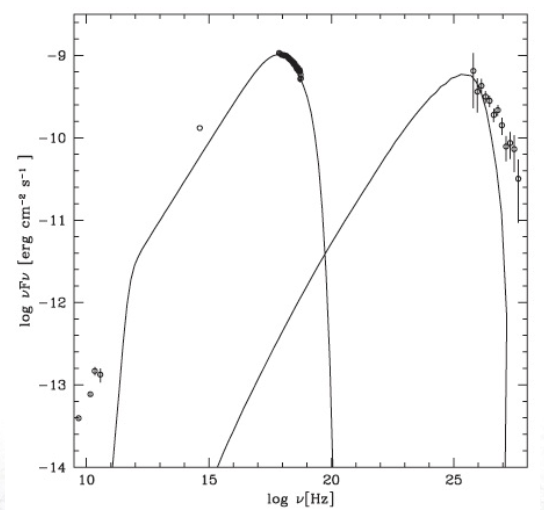
\includegraphics[width=7cm]{figures/figure1_9.png}
\captionsetup{justification=raggedright, singlelinecheck=false}
\caption{同步加速辐射和 SSC 能谱示意图。}
\label{同步加速辐射和 SSC 能谱示意图。}
\end{figure}

图\ref{同步加速辐射和 SSC 能谱示意图。}就展示了同步加速辐射和 SSC 能谱。可以发现左侧能谱左侧第一段受到同步加速辐射自吸收的影响。第二段的谱指数则与 SSC 一致。同步加速辐射第三段以$\mathrm{e}$指数下降,而右侧 SSC 能谱则在高能处截断。因此光谱中能观测到双峰分布,根据 (\ref{1.2.35})(\ref{1.2.48}) 式可知二者峰值比为
\begin{equation}
\frac{P_{\text{sync}}}{P_{\text{ICS}}}=\frac{\left.\nu F_{\nu}\right\vert{}_{\text{sync}}}{\left.\nu F_{\nu}\right\vert{}_{\text{ICS}}}=\frac{U_{B}}{U_{\text{rad}}}.
\end{equation}
其中已经用到了$\beta\to1$的假定,可见峰值反映了磁场和辐射场的比值。

\subsubsection{正负电子对产生与湮灭}
电子{}-{}正电子对在湮灭时会产生双光子。在电子静止系中观察,能量为$\gamma m_{0}c^{2}$的正电子和静止电子的湮灭截面为
\begin{equation}
\sigma_{\text{湮灭}}=\frac{\pi r_{0}^{2}}{\gamma+1}\left[\frac{\gamma^{2}+4\gamma+1}{\gamma^{2}-1}\cdot \ln\left(\gamma+\sqrt{\gamma^{2}+1}\right)-\frac{\gamma+3}{\sqrt{\gamma^{2}-1}}\right].
\end{equation}
低速极限下上式接近
\begin{equation}
\sigma_{\text{湮灭}}=\pi r_{0}^{2}\left(\frac{v}{c}\right)^{-1}.
\end{equation}
正电子速度$v\to0$情形下,截面发散,不过湮灭概率$R$应该依旧有限。设电子密度$N_{e}$,则每秒湮灭次数应该为
\begin{equation}
R=N_{e}\sigma_{\text{湮灭}}v=\pi r_{0}^{2}cN_{e},
\end{equation}
我们知道汤姆孙散射截面是$\dfrac{8}{3}\pi r_{0}^{2}$,光速$v=c$,因此正电子被电子湮灭速率和光子被电子散射速率是差不多的。而高速情形下的湮灭截面为
\begin{equation}
\sigma_{\text{湮灭}}=\frac{\pi r_{0}^{2}}{\gamma}\left(\ln\left(2\gamma\right)-1\right).
\end{equation}
可见高能正电子的湮灭截面很小。而此截面也与极端相对论情形下的康普顿散射截面很接近。

电子对湮灭产生的两光子一般不具有相同频率。极端相对论情况下,向前方射出的光子几乎取走全部正电子能量,而第二个光子能量近似只有$m_{0}c^{2}$的量级,且从后方射出。

电子对湮灭的逆过程,双光子湮灭产生电子对,同样有重要的作用。在许多 AGN 的喷流 (jet) 与冕 (corona) 中,$\gamma$光子和 X 射线光子(高能提供能量,低能保证散射截面足够大,都高能或都低能不利于湮灭)碰撞会产生电子对 (pair production),造成$\gamma$射线出射强度显著减弱,同时导致正负电子会在中心黑洞某些区域集中,引起小区域的光变。极端相对论情况下,湮灭截面为
\begin{equation}
\sigma_{\text{湮灭}}=\pi r_{0}^{2}\left(\frac{m_{0}c^{2}}{\hbar\omega_{0}}\right)^{2}\left[\left(2\ln2\right)\left(\frac{\hbar\omega_{0}}{m_{0}c^{2}2}\right)-1\right].
\end{equation}
如果是两个伽马光子碰撞,典型散射截面大小为$0.2\sigma_{\text{T}}$.当
\begin{equation}
l_{\text{X-ray}}=\frac{L_{\text{X-ray}}\sigma_{\text{T}}}{4\pi m_{0}c^{3}R}\gg\frac{h\nu_{\text{X-ray}}}{m_{0}c^{2}}
\end{equation}
时伽马光子就很难不与 X 射线光子湮灭,基本上无法从区域中逃离。其中$R$是源半径,$l$又被称作 compactness parameter,描述了光深。

AGN 中电子产生与湮灭速率可以平衡,康普顿厚 (compton-thick, CT, 指氢原子柱密度达到$10^{24}\,\mathrm{cm^{-2}}$) 的等离子体温度可以达到$10^{9}\,\mathrm{K}$,提供了电子产生和湮灭的环境。

单个高能光子有足够的能量也能产生电子对,不过此时为了满足能量和动量守恒必须有其他粒子在场,因此高频光子在等离子体场中穿行也是损失能量的重要原因之一。

还有一种对高能光子的重要吸收机制,即高能光子穿越强磁场时,被磁场吸收转化为正负电子对,其辐射吸收系数为
\begin{equation}
k=\frac{m_{0}c}{\hbar}\alpha\frac{B\sin\theta}{2B_{c}}\frac{1}{4}\left(\frac{3}{2}\right)^{\frac{1}{2}}\exp\left[-\frac{8m_{0}c^{2}B_{c}}{3EB\sin\theta}\right],
\end{equation}
其中精细结构常数$\alpha=\dfrac{e^{2}}{\hbar c}$,中子星临界磁场$B_{c}=\dfrac{m_{0}c^{3}}{e\hbar},\theta$是光子传播路径与磁场的夹角。

\subsubsection{轫致辐射}
轫致辐射来自电子受库仑场影响骤然改变速度的过程,而最常见的库仑场自然是等离子体中另一个离子的库仑场。不过严格来讲轫致辐射是量子过程,而量子理论中,电子和离子的组合可以看作是一个处于“自由态”的粒子,辐射出一个光子电子态就从一个自由态跃迁到另一个自由态,故也被称作自由{}-{}自由跃迁。这种意义上轫致辐射其实也算热辐射的一种。

一般仅考虑电子和正离子的碰撞。查阅\textit{Radiative Processes in Astrophysic} by George B. Rybicki 可知,速度服从 Maxwell 分布,温度为$T$的等离子体,发射率为
\begin{equation}
4\pi j_{\nu}=\frac{2}{\pi}mc^{2}\sigma_{\text{T}}^{\frac{3}{2}}\left(\frac{mc^{2}}{k_{\text{B}}T}\right)^{\frac{1}{2}}Z^{2}n_{e}n_{i}\exp\left(-\frac{h\nu}{k_{\text{B}}T}\right)\overline{g}_{\text{ff}}\left(T,Z,\nu\right),
\end{equation}
其中$Z$是离子电荷数,$\overline{g}_{\text{ff}}$是对速度作平均后的 Gaunt 因子。将$\overline{g}_{\text{ff}}$进一步对频率作平均后得到$\overline{g}_{B}$,单位体积的功率为
\begin{equation}
C_{\text{ff}}=\left(\frac{2\pi k_{\text{B}}T}{3m}\right)^{\frac{1}{2}}\frac{2^{5}\pi e^{6}}{3hmc^{3}}Z^{2}n_{e}n_{i}\overline{g}_{B}.
\end{equation}

我们提到轫致辐射可看作是热辐射,因此吸收系数近似满足
\begin{equation}
\alpha_{\nu}=\frac{j_{\nu}}{B_{\nu}\left(T\right)},
\end{equation}
$h\nu\gg k_{\text{B}}T$时$\alpha_{\nu}\propto{}\nu^{-3}$, $h\nu\ll k_{\text{B}}T$时$\alpha_{\nu}\propto{}\nu^{-2}$.因此低频波段光学厚,光谱是电子温度的黑体谱的 Rayleigh-Jeans 近似。而高频波段光学薄,谱形状与黑体谱很不一样,由 Gaunt 因子决定,近似平谱。

对于电离氢来说,$Z=1,n_{e}=n_{i}$,用吸收系数计算出的光深近似公式为
\begin{equation}
\tau_{\nu}\approx8.235\times10^{-2}T_{e}^{-1.35}\nu^{-2.1}\int n_{e}^{2}\mathrm{d}l.
\end{equation}

前文提到单个高能光子可以产生电子对,它和轫致辐射结合是宇宙线 (cosmic ray) 中电⼦{}-{}光⼦级联簇射的原因。能量极⾼的$\gamma$光⼦(例如可通过介⼦的衰变得到)穿过介质⽽产生⾼能电⼦对,这些电子又通过轫致辐射失去部分能量,产⽣次级光⼦,这些$\gamma$光⼦又进一步产⽣电⼦对。

\subsubsection{线谱}
原子物理告诉我们,组成物质的原子或分子有特定的能级,能级发生跃迁时,将会释放或吸收光子,产生线谱。每种物质都有属于自己的特征谱线,因此可通过光谱鉴别物质的化学组成。而光传播路径上物质越多,辐射或吸收的光子越多,谱线高度或深度越大,因此可根据谱线强度推断物质的密度。

原子谱线可能是最为常见的谱线。依据释放或吸收能量及跃迁前后电子是否与原子复合可将跃迁过程分为五种:吸收、发射、电离、复合、自由{}-{}自由跃迁。如果电子被完全电离,可以将电子看作是连续态,因为此时电子能量不必局限于特定值,故电离、复合、自由{}-{}自由跃迁是连续谱。
\begin{figure}[!htbp]
\centering
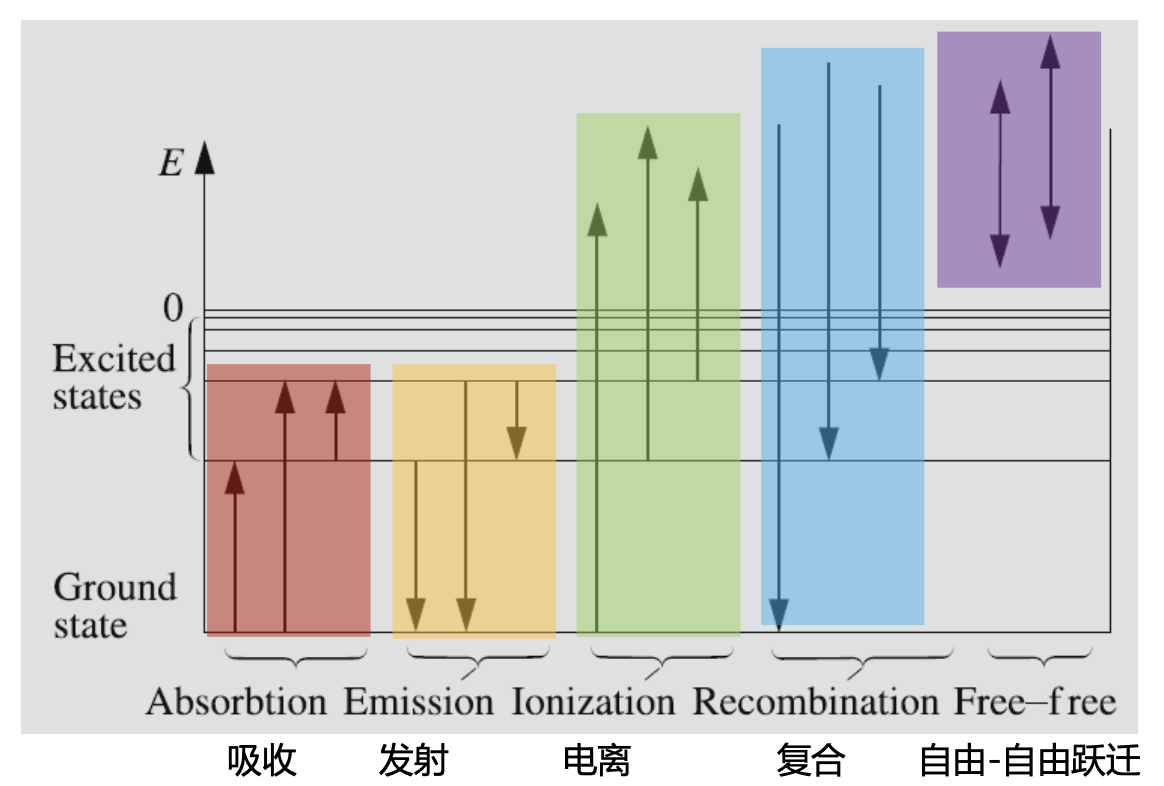
\includegraphics[width=8.3cm]{figures/figure1_10.png}
\captionsetup{justification=raggedright, singlelinecheck=false}
\caption{不同的电子跃迁过程。}
\label{不同的电子跃迁过程。}
\end{figure}

对于吸收和发射谱线,可以根据跃迁能级将谱线划分为不同的线系,以氢原子为例,不同能级间的能量差满足
\begin{equation}
\Delta{}E=13.6\,\mathrm{eV}\left(\frac{1}{n^{2}}-\frac{1}{m^{2}}\right),
\end{equation}
$n=1,2,3,4$所对应的线系分别为 Lyman, Balmer, Paschen, Brackett 线系,具体如图\ref{氢原子的不同线系。}所示。

\begin{figure}[!htbp]
\centering
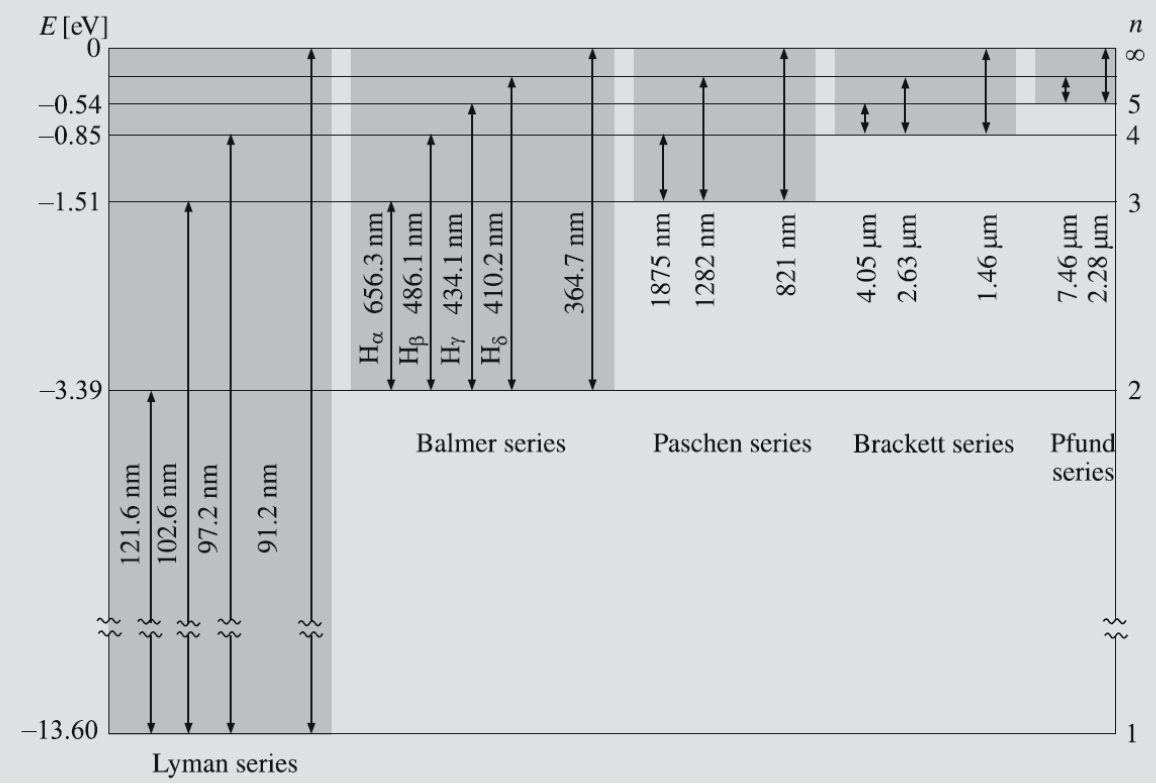
\includegraphics[width=10cm]{figures/figure1_11.png}
\captionsetup{justification=raggedright, singlelinecheck=false}
\caption{氢原子的不同线系。}
\label{氢原子的不同线系。}
\end{figure}

以 Balmer 线系为例,自第一激发态跃迁到第二激发态时需要吸收波长为$656.3\,\mathrm{nm}$的光子,而恒星大气中有氢元素,因此恒星光谱中可以产生$\mathrm{H\alpha}$吸收线。当光子能量逐渐提高,波长短于$364.6\,\mathrm{nm}$时,电子可以被完全电离,光子都可以被处于第一激发态的氢原子吸收,因此产生连续的吸收谱。如图\ref{Balmer break.}所示,因为光谱在这一波长附近出现明显的下降,仿佛光谱发生了断裂,被称作 Balmer break.这个特征在天文学中非常重要,特别是在研究恒星和星系的年龄和金属丰度时。前文提到的 uvby 四色测光便研究了这一特征。
\begin{figure}[!htbp]
\centering
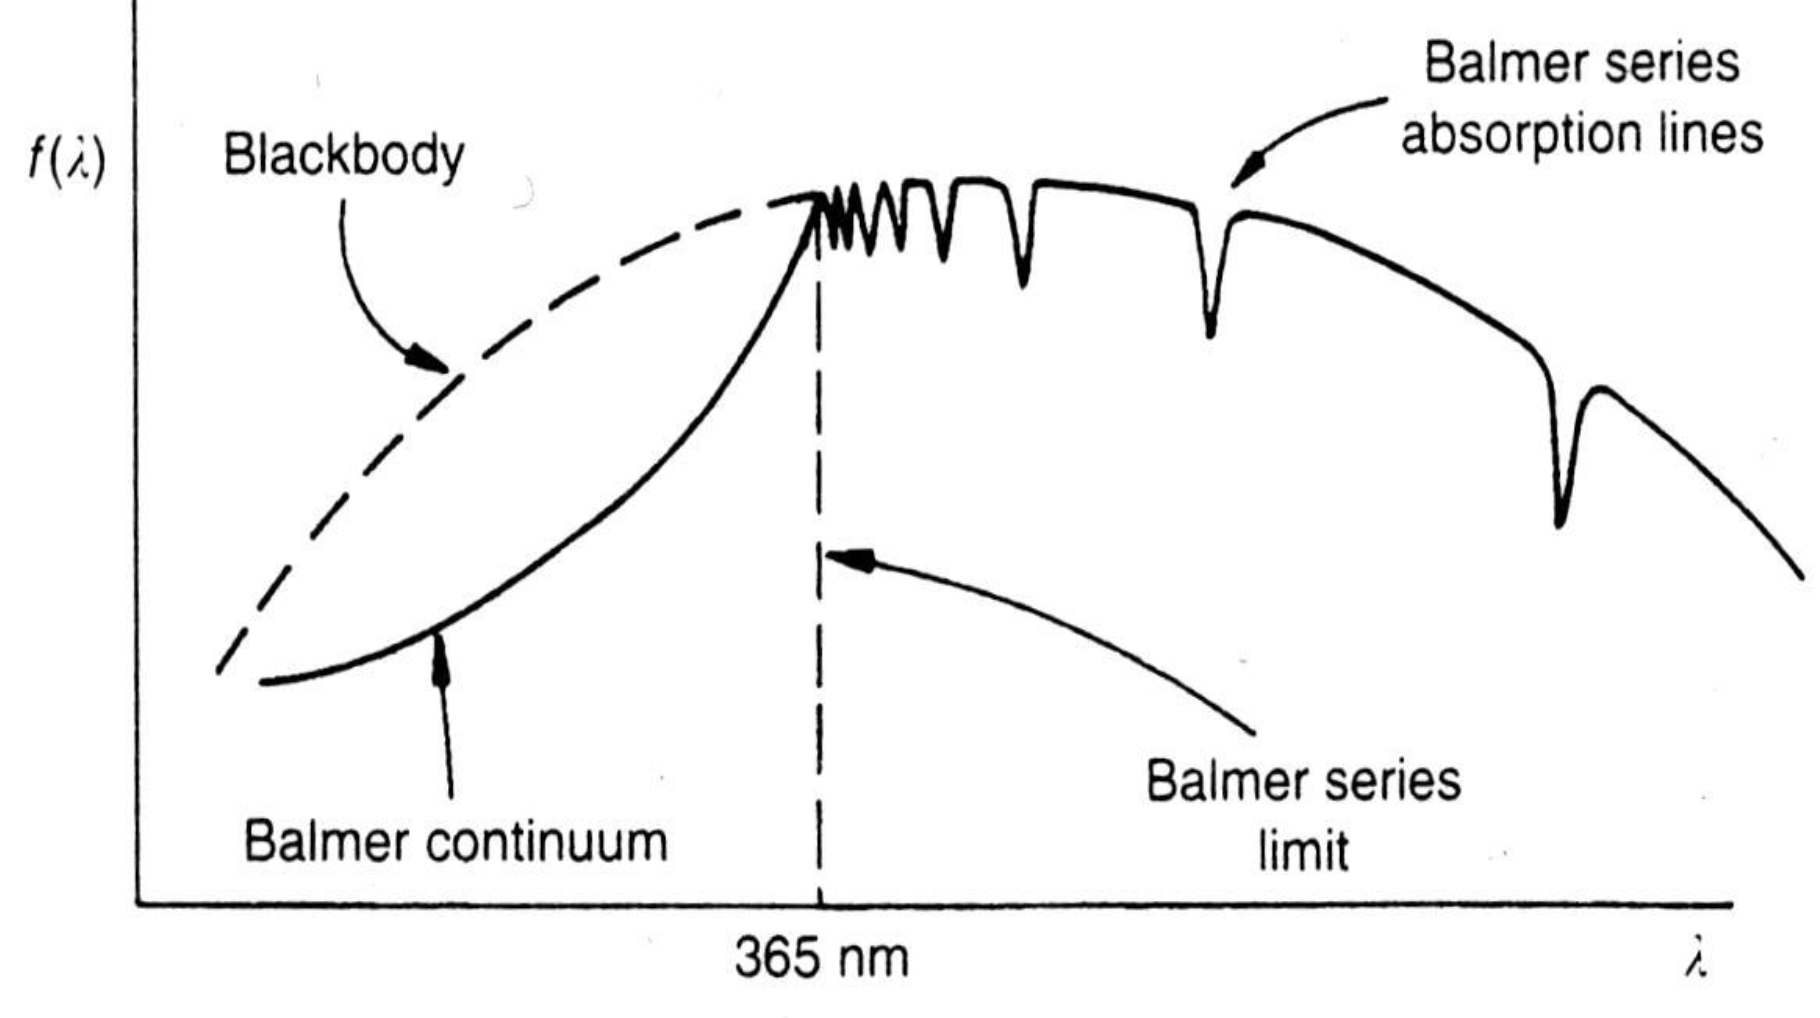
\includegraphics[width=8cm]{figures/figure1_12.png}
\captionsetup{justification=raggedright, singlelinecheck=false}
\caption{Balmer break.}
\label{Balmer break.}
\end{figure}

上述所讲的是吸收线。发射线的一般图景是,电子与原子或离子发生非弹性碰撞时,原子或离子被激发,又回到基态,发射碰撞激发线。要看见这种谱线,需要自发辐射时标小于碰撞时标(否则又被撞回去了),因此自发辐射要迅速,且气体密度要非常低,通常每立方厘米只有几千个粒子。

前文曾提到热辐射源自粒子能量通过电磁相互作用的量子化释放。实际上,研究这种能级跃迁我们需要研究粒子哈密顿量 (Hamiltonian) 在电磁场下的含时演化,最终计算得到的跃迁概率,其一阶展开可看作是原子电偶极矩与外界电场相互作用的结果,被称作电偶极辐射,也就是上述由主量子数$n$所定的原子谱线。电偶极辐射只涉及到电子的轨道运动,因此仅由主量子数决定,服从选择定则,要求轨道量子数和磁量子数变化满足$\Delta{}l=\pm1,\Delta{}m_{l}=0,\pm1$.

而其他高阶项展开可以得到磁偶极矩和电四极矩辐射。这些类型的辐射被称作禁戒跃迁,意为跃迁概率很小。禁戒跃迁不服从电偶极辐射的选择定则,只能发生于密度非常低的环境。地球上禁线不可能出现,一是禁线$A_{ik}$太小,自发辐射时标$>1\,\mathrm{s}$,太长了,与之相比电偶极辐射对应的原子能级寿命往往小于$10^{-8}\,\mathrm{s}$.二是人类的真空科技点太低,实验室制造的真空气体密度远高于宇宙的超真空 (<$1\,\mathrm{atom\cdot cm^{-3}}$).禁线强度非常强烈地依赖于发射禁线气体的密度和温度,因此可用来确定星系发射线区的密度和温度。一般用方括号包裹元素符号来标记禁线。如$\lambda=5007\,\si{\angstrom}$的$\mathrm{[O\,\uppercase\expandafter{\romannumeral3}]}$线。值得注意的是,\uppercase\expandafter{\romannumeral3}表示失去了两个电子,因此类似$\mathrm{H\,\uppercase\expandafter{\romannumeral1}}$的符号其实表示的是中性原子。后续会反复用到这种表示法。

源自原子精细结构和超精细结构的辐射属于禁戒跃迁。精细结构来自电子自旋和轨道角动量产生的磁矩之间的相互作用。对应能量差只有主能级能量差的$\dfrac{1}{137^{2}}$,辐射集中在远红外区域。超精细结构是核自旋和轨道电子自旋产生的磁场之间的耦合结果。能级分类比精细结构谱线还要小 2000 倍。辐射甚至来到射电的厘米波段。如$21\,\mathrm{cm}$谱线来自氢原子中电子自旋和原子核自旋处于平行状态(能量更高)向反平行状态的禁戒跃迁,时标$10^{7}\,\mathrm{yr}$.尽管单个氢原子的跃迁概率极低,但由于星际空间中的中性氢非常丰富,其产生的$21\,\mathrm{cm}$谱线仍然能够观测到。由于射电波段受尘埃的影响小,因此$21\,\mathrm{cm}$线是研究星系结构的重要手段。

当星际间的物质温度较低 ($T<100\,\mathrm{K}$) 时,原子不足以达到激发态,难以产生强发射线。好在分子振动和转动同样会发出辐射。转动跃迁集中在射电波段,振动跃迁则集中在红外波段。转动跃迁往往要求分子具有永久的偶极矩,这不是个好消息,因为我们比较关注宇宙中的氢元素,而对称分子的辐射较弱。但好在,$\mathrm{CO}$分子往往和氢分子一起出现,且丰度仅次于氢分子,$1.3\,\mathrm{mm}$和$2.6\,\mathrm{mm}$的转动跃迁在密度$n(\mathrm{H}_{2})\sim100\text{\textendash}1000\,\mathrm{cm^{-3}}$通常最强,因此可以利用$\,\mathrm{CO}$的毫米射电辐射可以研究氢分子的分布。分子转动谱线还有个非常有趣的特点。具体转动能级的能量满足
\begin{equation}
E=\frac{J(J+1)}{2I}\hbar^{2},
\end{equation}
其中$J$是量子数,$I$描述了分子的转动惯量。对于三个相邻的能级来说
\begin{equation}
\Delta{}E_{J+1\to J}=\frac{\left(J+1\right)}{I}\hbar^{2},\Delta{}E_{J\to J-1}=\frac{J}{I}\hbar^{2},\Delta{}E_{J+1\to J}-\Delta{}E_{J\to J-1}=\frac{\hbar^{2}}{I}.
\end{equation}
因此辐射线心频率等间距,而原子谱线,如图\ref{氢原子的不同线系。}所示,在接近线系极限处会越来越密。

我们已经介绍了常见的谱线类型,接下来要介绍,在具体的光谱观测中,我们需要注意哪些观测量,以及这些观测量能告诉我们哪些天体物理信息。相对连续谱,谱线带有宝贵的速度信息,有助于了解辐射过程和辐射源的动力学特征。

首先要关注的自然是谱线的强度(或深度)。以吸收线为例,天体光谱是连续谱与吸收线的叠加,在吸收线所在位置,先构造出伪连续谱。
\begin{figure}[!htbp]
\centering
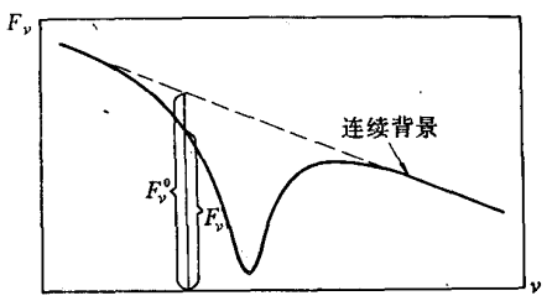
\includegraphics[width=8cm]{figures/figure1_13.png}
\captionsetup{justification=raggedright, singlelinecheck=false}
\caption{伪连续谱与吸收线。}
\label{伪连续谱与吸收线。}
\end{figure}

吸收线的辐射强度记作$I_{\nu}$,伪连续谱辐射强度记作$I_{\nu}^{0}$.可以定义剩余强度
\begin{equation}
r_{\nu}=\frac{I_{\nu}}{I_{\nu}^{0}},
\end{equation}
以及线深度
\begin{equation}
R_{\nu}=1-r_{\nu}.
\end{equation}
可见线深度描述了,被物质吸收的那部分辐射强度相对连续谱强度的大小,因此对其进行积分就描述了物质的吸收能力。定义总吸收为
\begin{equation}
W_{\nu}=\int_{\nu_{1}}^{\nu_{2}}R_{\nu}\mathrm{d}\nu.
\end{equation}
辐射强度也可以用波长为单位,且恒星光谱实际测量中一般取波长标度,故可以给出以波长定义的总吸收,它与$W_{\nu}$的关系为
\begin{equation}
\frac{W_{\nu}}{\left\vert{}\Delta{}\nu\right\vert{}}=\frac{W_{\lambda}}{\left\vert{}\Delta{}\lambda\right\vert{}}.
\end{equation}
$W_{\lambda}$也被称作等值宽度 (equivalent width, EW),即与吸收(或发射)谱线轮廓和连续谱之间所包围的面积相当的高度为 1 的矩形的宽度。另一个重要的宽度是,线深度为最大值一半时,对应两个波长的宽度,即半高全宽 (full width at half maximum, FWHM).

接着要考虑的是谱线线心的频率大小,即谱线的位置。在《广义相对论基础》中我们介绍过光子的引力红移,它就改变了观测到的谱线频率。天文学中还存在两种红移,一种是多普勒红移,当物质朝向(远离)我们运动时,其辐射频率会蓝移(红移)。通过观测确定线心频率的位移程度,可以确定天体的视向速度。比如系外行星的引力会扰动恒星运动,可观测恒星光谱确定视向速度的变化发现系外行星。以这种方式发现的行星大多质量较大,公转轨道半径小,多是热木星,毕竟这样对恒星的扰动才比较大。另一种红移是宇宙学红移,由宇宙膨胀引起波长拉伸。观测到的谱线频率是三者的综合作用:
\begin{equation}
\lambda_{\text{obs}}=\lambda_{0}\left(1+z_{\text{gravity}}\right)\left(1+z_{\text{doppler}}\right)\left(1+z_{\text{cosmology}}\right).
\end{equation}
对于宇宙学红移,本章第六节将会简要介绍。

多普勒红移结合多普勒运动引起的辐射强度变化会改变谱线轮廓。比如 AGN 吸积物质时,由于角动量守恒被吸积的物质会构成一个高速转动的吸积盘,beaming effect 和多普勒效应会共同导致吸积盘的一半比另一半亮得多,同时光谱中 Fe 元素谱线的轮廓极度不对称。

最后要考虑的则是谱线的宽度。现代天文研究中谱线宽度相当重要,能告诉我们很多天体物理信息。首先,量子力学告诉我们,$\Delta{}E\Delta{}t>\dfrac{h}{4\pi}$,即原子停留在某一能级的所具有的能量值有不确定值,因此谱线不能是无限窄的,而是有一宽度,这被称作自然展宽。第二种宽度来自多普勒效应,以吸收线为例,如果光子能量低于能级差,光子无法被原子吸收,但如果原子具有热运动,其与光子双向奔赴,动能填补了能量差,即使光子能量较低也能被吸收。在吸收线谱中则表现为频率较低的部分也被吸收,因此谱线变宽。原子间的碰撞也会导致谱线变宽,而碰撞次数多意味着压力更大,因此可通过谱线宽度确定气压大小,而后者和恒星的引力大小有关。除此之外,磁场(塞曼效应)和电场(斯塔克效应)也会导致谱线变宽或分裂。多普勒展宽得到的谱线形状是高斯型,碰撞展宽是洛伦兹型。实际观测得到的谱线轮廓,一般中心以高斯轮廓为主,线翼以洛仑兹轮廓为主。有关致宽机制更具体的细节可以翻阅《恒星大气物理》(汪珍如、曲钦岳)。高斯型和洛伦兹型谱线轮廓可大致如图\ref{高斯型和洛伦兹型谱线轮廓。}所示,可以发现洛伦兹型谱线轮廓的线翼更宽。
\begin{figure}[!htbp]
\centering
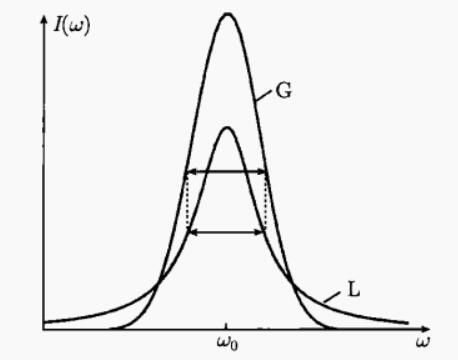
\includegraphics[width=7cm]{figures/figure1_16.jpg}
\captionsetup{justification=raggedright, singlelinecheck=false}
\caption{高斯型和洛伦兹型谱线轮廓。}
\label{高斯型和洛伦兹型谱线轮廓。}
\end{figure}

\subsection{恒星简介}
\subsubsection{金属丰度表示法}
我们已经了解了关于电磁辐射的大部分知识。对于宇宙中大部分天体,我们都是通过图像和光谱了解其物理信息的,包括天体的面亮度、光度、大小、距离、年龄、温度和化学成分。比如,结合光谱特征谱线的种类和强度可以确定恒星或星际气体和尘埃的温度和金属丰度。金属丰度常用以下三种方法表示:

1. 以质量分数表示,比如可直接记氧元素含量为$\mathrm{O}=0.02$.

2. 按原子数目比表示,任意金属(天文学中氢氦以外的元素都是“金属”)$\mathrm{Z}$的含量为
\begin{equation}
\log(\mathrm{Z}/\mathrm{H})+12=\log(N_{\mathrm{Z}}/N_{\mathrm{H}})+12.
\end{equation}

3. 按相对太阳的元素丰度
\begin{equation}
[A/B]=\lg\,[\frac{(\textrm{number\,of\,A\,atoms/number\,of\,B\,atoms})_{\mathrm{star}}}{(\textrm{number\,of\,A\,atoms/number\,of\,B\,atoms})_{\mathrm{\odot}}}],
\end{equation}
因此$[\mathrm{Fe/H}]=-2$的恒星,其铁丰度就是太阳的$1\%$.一般来讲$[\mathrm{Fe/H}]$等价于一颗恒星相对于太阳的平均重元素丰度。

\subsubsection{恒星分类系统与赫罗图}
进一步,我们可以根据恒星的这些特征对其进行分类。早期天文研究中人们用 Balmer 线系吸收线的强度确定恒星的温度,因为恒星温度越高,从基态来到第一激发态的氢原子就越多,能吸收的 Balmer 光子也就越多,吸收线就越强。于是人们根据吸收线强度从高到低将恒星排成 ABCD……但后来发现这样分类有问题,因为温度再高一点电离程度提高,Balmer 线所对应的第一激发态原子数反而变少,因此字母顺序不一定对应温度顺序。在漫长的观测中,哈佛大学天文台逐渐完善了哈佛光谱分类系统,基于光谱特征谱线和谱带的种类、等值宽度、强度比值和连续谱的能量分布进行分类。它以温度为一元参量,按有效温度从高到低,将恒星分为七个光谱型,OBAFGKM,每型又分为十个次型,用阿拉伯数字表示,比如太阳是 G2 型恒星。人们常用``Oh, be a fine girl/guy kiss me!''来记忆哈佛光谱型。(如果你不确定对面是否学过天文兴许能用这句话作为接头暗号。)常把 O、B、A 型恒星叫作早型恒星,F、G 型叫作中型,K、M 型叫作晚型。星系光谱是由不同温度恒星的光谱混合而成的,较热的恒星(早型恒星)贡献了大部分的蓝光。较冷的恒星贡献了大部分的红光。每个光谱型的有效温度和特征谱线如表\ref{哈佛}所示。后来哈佛分类系统还添加了 R、N 分支以反映恒星化学成分的差别。

后来人们发现,仅靠温度进行恒星分类还不够。对于同一光谱型(即有效温度相同)的恒星,其光度可以有很大的差异,暗示着这些恒星的物理结构完全不同。于是 Yerkes 天文台的 William W. Morgan 和 Philip C. Keenan 等人引入 MK 分类(又称 Yerkes 分类)。它采用温度和光度二元参量,将恒星进一步分类为主序星、白矮星、巨星等等。MK 分类如表\ref{Yerkes}所示。太阳是 G2V 恒星。

\begin{table}[!htbp]
\centering
\caption{哈佛光谱分类系统。}
\begin{tabular}{c c c c}
\hline
光谱型 & 有效温度 & 颜色 & 特征谱线\\
\cline{1-4}
O & $30000\,\mathrm{K}$ & 蓝 & 强电离$\mathrm{He}$线、重元素多次电离线\\
\cline{1-4}
B & $20000\,\mathrm{K}$ & 蓝白 & 中性$\mathrm{He}$线,重元素一次电离线,$\mathrm{H}$线\\
\cline{1-4}
A & $10000\,\mathrm{K}$ & 白 & 重元素一次电离线,$\mathrm{H}$线\\
\cline{1-4}
F & $7000\,\mathrm{K}$ & 黄白 & 中性金属线,重元素一次电离线,$\mathrm{H}$线\\
\cline{1-4}
G & $6000\,\mathrm{K}$ & 黄 & 中性金属线,重元素一次电离线\\
\cline{1-4}
K & $4000\,\mathrm{K}$ & 红橙 & 中性金属线,重元素一次电离线\\
\cline{1-4}
M & $3000\,\mathrm{K}$ & 红 & 中性金属线、分子带\\
\cline{1-4}
\end{tabular}
\label{哈佛}
\end{table}

\begin{table}[htbp]
\centering
\caption{MK 分类。}
\begin{tabular}{c c}
\hline
\uppercase\expandafter{\romannumeral 1}a & Very luminous supergiants\\
\cline{1-2}
\uppercase\expandafter{\romannumeral 1}b & Less luminous supergiants\\
\cline{1-2}
\uppercase\expandafter{\romannumeral 2} & Luminous giants\\
\cline{1-2}
\uppercase\expandafter{\romannumeral 3} & Giants\\
\cline{1-2}
\uppercase\expandafter{\romannumeral 4} & Subgiants\\
\cline{1-2}
\uppercase\expandafter{\romannumeral 5} & Main sequence stars (Dwarf stars)\\
\cline{1-2}
\uppercase\expandafter{\romannumeral 6} & Subdwarf\\
\cline{1-2}
\uppercase\expandafter{\romannumeral 7} & White dwarf\\
\cline{1-2}
\end{tabular}
\label{Yerkes}
\end{table}

有了温度和光度二元分类,我们很自然地引入赫罗图的概念。如图\ref{赫罗图。}所示,我们将观测到的恒星绘制在以温度和光度为坐标轴的二维平面上,其中横轴是温度,左高右低,纵轴是光度,上高下低,可以发现恒星大致分为三个区域。其一是从赫罗图左上方延伸至右下方的窄带,绝大部分恒星坐落其中,该窄带被称作主序带。主序带恒星拥有均匀的化学组成,稳定的核心氢燃烧,完全流体静力学平衡,质量范围$\sim0.08\text{\textendash}120M_{\odot}$(质量低不足以点燃氢核聚变,质量太高动力学不稳定)。其二是赫罗图左下方温度极高亮度极低的白矮星,其三是赫罗图右上方温度较低光度极高的巨星。读者朋友可能有疑问,为什么温度高(低)光度反而低(高)。答案是白矮星半径太小 ($10^{-2}\text{\textendash}10^{-1}R_{\odot}$),巨星半径太大 ($10\text{\textendash}1000R_{\odot}$),而光度满足$L=4\pi R^{2}\sigma_{\text{SB}}T^{4}$,且温度差异的数量级不显著影响较小。同时在图\ref{赫罗图。}左半部分上方还能看到哈佛光谱型,赫罗图直观展示了同一光谱型可能对应不同类型恒星的事实,因此有必要引入 MK 分类。根据光度公式可在赫罗图上绘制等半径线$\log\left(R/R_{\odot}\right)=\log\left(L/L_{\odot}\right)/2-2\log\left(T/T_{\odot}\right)$.图\ref{赫罗图。}中更多的名词解释我们将在后续恒星演化部分提及。

\begin{figure}[!htbp]
\centering
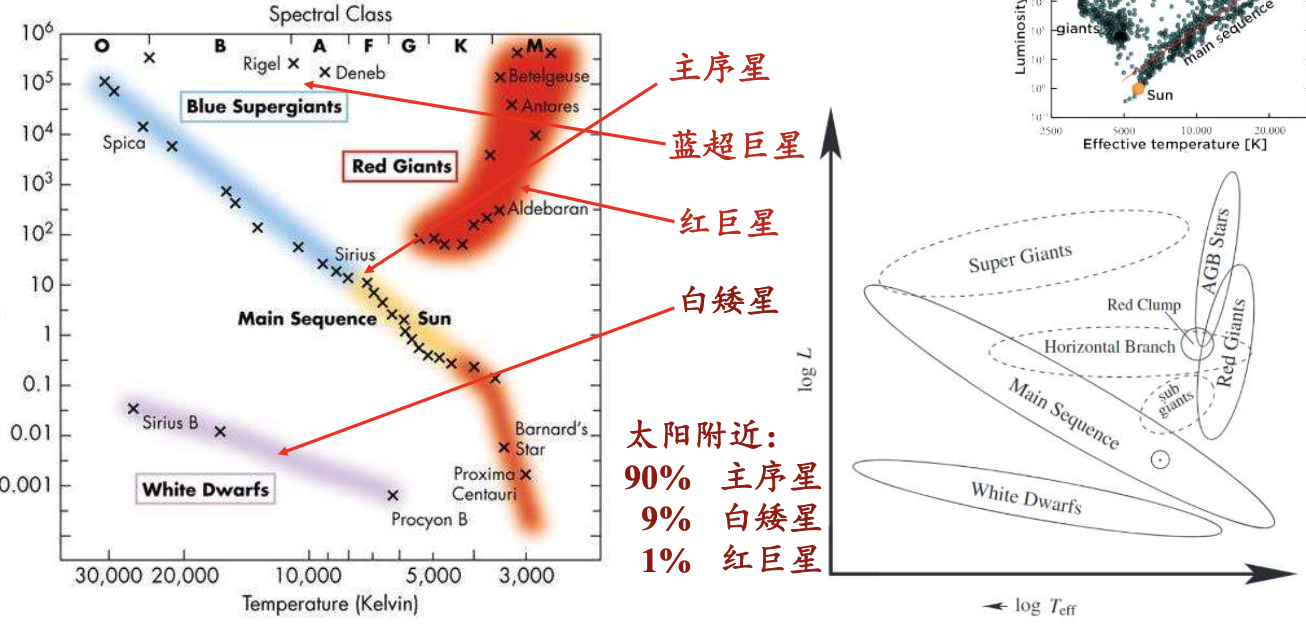
\includegraphics[width=14cm]{figures/figure1_14.png}
\captionsetup{justification=raggedright, singlelinecheck=false}
\caption{赫罗图。}
\label{赫罗图。}
\end{figure}

\subsubsection{质光关系}
我们发现在赫罗图中主序星跨越了 OBAFGKM 整个哈佛光谱型范围,光度和温度跨越极大,但是 MK 分类中将其分为一种,这背后有什么物理原因吗?实际上人们在观测中确实发现主序星之间性质的联系,这便是本小节要介绍的质光关系。质光关系源自对恒星模型的大致近似。对于一个稳定燃烧的恒星,我们假设其处于流体静力学平衡,即
\begin{align}
\frac{\mathrm{G}M_{r}\rho\mathrm{d}A\mathrm{d}r}{r^{2}}&=\mathrm{d}P\mathrm{d}A,\\
\frac{\mathrm{d}P}{\mathrm{d}r}&=\frac{\mathrm{G}M_{r}\rho}{r^{2}}.\label{1.4.4}
\end{align}
于是我们大概得知两种关系,$\dfrac{P}{R}\sim\dfrac{M\rho}{R^{2}},\rho\sim\dfrac{M}{R^{3}}$,并由此推出$P\sim\dfrac{M^{2}}{R^{4}}$.我们一般假设恒星内部气体遵循理想气体状态方程,即$P=\dfrac{\rho k_{\text{B}}T}{\mu m_{\mathrm{H}}}$,其中$\mu$是相对分子质量,$m_{\mathrm{H}}$是氢原子质量,由此得到$T\sim\dfrac{M}{R}$.与引力相抗衡的压力有辐射压和气压两种,此处我们只考虑辐射压存在,可进一步建立辐射压和温度的关系。我们曾介绍过球对称情况下的能量密度,对于黑体辐射,
\begin{equation}
U_{\nu}=\frac{4\pi{}}{c}B_{\nu}=\frac{8\pi\nu^{2}}{c^{3}}\cdot\frac{1}{e^{\frac{h\nu}{k_{\text{B}}T}}-1}\cdot h\nu.
\end{equation}
对频率积分可以得到总能量密度:
\begin{equation}
U=\int\varepsilon\left(\nu\right)\mathrm{d}\nu=\frac{8\pi h}{c^3}\int\frac{\nu^3\mathrm{d}\nu}{e^{\frac{h\nu}{k_{\text{B}}T}}-1}=\frac{8\pi}{c^3}\frac{k_{\text{B}}^4T^4}{h^3}\int\frac{x^3\mathrm{d}x}{e^{x}-1}=\frac{8\pi^{5}k_{\text{B}}^{4}}{15h^{3}c^{3}}T^{4}=a_{\text{B}}T^4.
\end{equation}
而流量满足(仅考虑向外辐射部分,进而可通过$F=\dfrac{L}{4\pi R^{2}}$确定系数)
\begin{align}
F_\nu&=\int I_\nu\cos\theta\mathrm{d}\Omega\notag\\
&=\int_0^{2\pi}\mathrm{d}\varphi\int_0^{\frac{\pi}{2}}\frac{c}{4\pi}U_\nu\cos\theta\sin\theta\mathrm{d}\theta\notag\\
&=\frac{c}{4}U_\nu\int_0^{\frac{\pi}{2}}\sin\left(2\theta\right)\mathrm{d}\left(2\theta\right)=\frac{c}{4}U_\nu.\\
\therefore F&=\frac{c}{4}a_{\text{B}}T^4,\sigma_{\text{SB}}=\frac{ca_{\text{B}}}{4}.
\end{align}
辐射压(要考虑各向同性贡献,因此积分限有变化)满足
\begin{align}
P_{R,\nu}&=\frac{1}{c}\int_{4\pi{}}I_{\nu}\cos^{2}\theta\mathrm{d}\Omega\notag\\
&=\frac{1}{c}\int_{0}^{2\pi{}}\mathrm{d}\varphi\int_{0}^{\pi}\frac{c}{4\pi{}}U_{\nu}\cos^{2}\theta\sin\theta\mathrm{d}\theta\notag\\
&=-\frac{1}{2}U_{\nu}\int_{0}^{\pi}\cos^{2}\theta\mathrm{d}\cos\theta=\frac{1}{3}U_{\nu},\notag\\
P_{\text{rad}}&=\frac{1}{3}a_{\text{B}}T^{4}.\label{1.4.9}
\end{align}
进一步地,我们可以建立起光度和质量的关系。在推导 Eddington 光度时我们曾经建立过有关光度和引力的方程,将其稍作修改可得
\begin{equation}
\frac{1}{c}\kappa\frac{L}{4\pi r^{2}}=\frac{\mathrm{G}M_{r}}{r^{2}},\label{1.4.10}
\end{equation}
联立 (\ref{1.4.4})(\ref{1.4.9})(\ref{1.4.10}) 式得到
\begin{align}
\frac{\mathrm{G}M}{r^{2}}=\frac{1}{\rho}\frac{\mathrm{d}P}{\mathrm{d}r}=\frac{1}{c}\kappa\frac{L}{4\pi r^{2}}=\frac{1}{\rho}\frac{4}{3}a_{\text{B}}T^{3}\frac{\mathrm{d}T}{\mathrm{d}r},\label{1.4.11}
\end{align}
由此可得
\begin{equation}
L\sim R^{2}\frac{1}{\rho}\frac{T^{4}}{R}\sim R^{2}\frac{R^{3}}{M}\frac{M^{4}}{R^{5}}\sim M^{3}.
\end{equation}
因此主序星存在质光关系,观测数据告诉我们$L\sim M^{2\text{\textendash}4}$.可以这么理解质光关系,恒星质量越大,引力越强,根据气体状态方程可知气体温度越高,因此光度更高。而辐射能实际上来自核反应,会消耗质量,因此恒星寿命$t\sim\dfrac{M}{L}\sim M^{-2}$,即质量越高,寿命越短。近邻宇宙中我们观测到的(意味着还活着的)恒星大部分质量较小,这是原因之一。

上述物理量间的关系还涉及到半径,我们希望消去这个因素。考虑到$L\sim R^{2}T^{4},T\sim\dfrac{M}{R}$,可以推得$M^{3}\sim M^{2}T^{2},M\sim T^{2},L\sim M^{3}\sim T^{6}$.因此光度、温度、压强、半径、密度等物理量仅与质量有关,质量是决定恒星物理属性的重要因素,它几乎完全决定了恒星的结构和最终命运。后续我们还将了解,如果恒星的初始质量和化学组分确定了,它的性质也就确定了。这被称作 Russell-Vogt Theorem.

读者朋友可能有疑问,那一颗大质量恒星燃烧过程中逐渐损失质量,不就变成小质量恒星,成功延年益寿了吗?我们提到过大质量恒星寿命短,所以观测上能看到的大质量恒星较少。反过来讲,大部分恒星处于主序带,因此恒星的一生主序星时期占比较长,恒星寿命主要由主序星阶段决定,而主序阶段的质量变化并不是特别显著,大质量恒星在主序阶段快要结束时才会剧烈抛射质量。已经平稳地度过一生,快死了回光返照并不能改变命运。进一步讲,热核反应本就不断改变恒星元素组成,即使变成小质量其核燃料也完全不同了,因此不能单纯认为寿命会变长。为定量研究这个问题,天文学家也引入了零龄主序 (Zero Age Main Sequence, ZAMS) 的概念,它是不同质量恒星刚进入主序阶段时在赫罗图上的位置集合,将其与实际观测数据作对比可以发现,恒星在主序带上占据一点后,会安静地燃烧直到自该点附近脱离主序。

质量和化学组分以不同的方式影响恒星寿命。质量较大的恒星中心区域温度和压力都非常高,核聚变反应进行得非常剧烈,因此燃料消耗速度非常快,寿命很短。而化学组分所起作用相对较小,它主要影响的是辐射转移的不透明度,金属丰度低,恒星中的尘埃就少,介质更透明,核反应更剧烈,光子从核心逃逸到表面也更容易,因此贫金属星更致密、核心更炽热、能产生更多的能量,更蓝更亮,寿命更短。比太阳亮的那部分主序带,宽度主要受年龄影响,较暗的部分宽度受金属丰度影响。

此外,基于主序星物理量之间的关系容易证明,质量不同的主序星表面重力加速度相差无几,因此主序星表面的压力对谱线宽度的影响较为一致,这也是 MK 分类中将主序星划分为一类的依据之一。

\subsubsection{\uppercase\expandafter{\romannumeral1}a 型超新星}
接下来简要说明一下\uppercase\expandafter{\romannumeral1}a 型超新星的图景。热核反应不断将恒星内部的轻元素转变为重元素,随着原子序数提高,库仑力会不断增强,需要更高的压力和温度以进行核反应。因此要点燃的元素越重,恒星所需的初始质量就越大。如果恒星质量不高,在初始氢燃料燃烧完毕留下一个高温的碳氧核心后核反应就停止了。不过,即使恒星初始质量极高,核反应也不能无限进行下去。根据质能关系可知原子核的结合能为$Q=\left[Zm_{\text{p}}+Nm_{\text{n}}-m_{Z,n}\right]c^{2}$,其中$Z$是质子数,$N$是中子数,$m_{Z,n}$是原子核质量。记原子量为$A=Z+N$,可以定义比结合能$Q/A$.铁元素拥有最大的比结合能,因此核聚变形成比铁元素重的元素时反而要消耗能量,核反应终究会停止。如此一来气压和辐射压不足以平衡引力,要维持恒星结构,必须由电子简并压抗衡引力,我们称这样的星体为白矮星。但电子简并压也不是无上限的,如果白矮星质量超过一定限度(称其为钱德拉塞卡极限),星体会进一步坍缩为中子星或黑洞。

于是我们可以考虑这样一种情形,在白矮星{}-{}恒星双星系统中,白矮星不断吸积伴星的物质,质量不断提高,直到超过钱德拉塞卡极限。此时星体会发生爆轰,整个星体彻底瓦解,什么也不剩下。我们称这样的星体为\uppercase\expandafter{\romannumeral1}a 型超新星。由于发生爆轰的 CO 核质量都差不多,因此峰值绝对星等都一致,大约$-19.5$等。因此可以用\uppercase\expandafter{\romannumeral1}a 型超新星测距。

\subsubsection{星团和星族}
恒星诞生自巨大气体云的坍缩,而同一朵气体云会诞生多个恒星,由此构成引力束缚的恒星系统。星团成员星都拥有相同的年龄和化学成分,因此演化差异几乎只与初始质量有关。我们已经了解质量越大的恒星寿命越短,意味着同一时期诞生的恒星,大质量的将会率先脱离主序向巨星演化。绘制此刻星团的赫罗图并与 ZAMS 对比确定拐点位置,可以判断此时是具有何种质量的恒星开始脱离主序,它的寿命就对应着星团年龄。具体可如图\ref{利用赫罗图和 ZAMS 判断星团年龄。}所示。
\begin{figure}[!htbp]
\centering
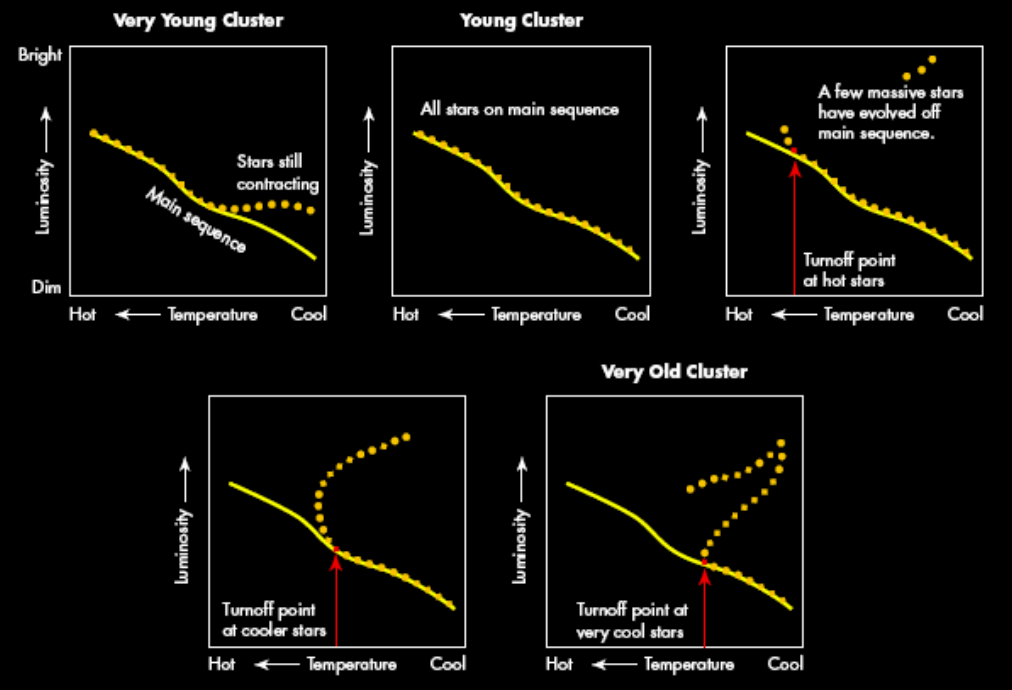
\includegraphics[width=12cm]{figures/figure1_17.png}
\captionsetup{justification=raggedright, singlelinecheck=false}
\caption{利用赫罗图和 ZAMS 判断星团年龄。}
\label{利用赫罗图和 ZAMS 判断星团年龄。}
\end{figure}

星团大小范围从几十颗恒星到几十万颗恒星,数量级差异巨大。人们将星团分为两种类型,疏散星团 (Open Cluster, OC) 和球状星团 (Globular Cluster, GC). OC 由数百至上千颗引力联系较弱的恒星组成,GC 成员可达数十万,恒星平均密度比太阳周围高数十倍。OC 成员星较为年轻,金属丰度高,GC 较为年老,金属丰度低。这暗示着它们诞生自宇宙的不同时期,因为金属是在漫长的核反应过程中诞生的,且在主序星死亡时才回归星际空间成为下一代恒星的原料。实际上人们还将恒星分类为星族\uppercase\expandafter{\romannumeral1}和星族\uppercase\expandafter{\romannumeral2}.星族是具有相似年龄、化学组成、空间分布和运动特性的恒星集合。星族\uppercase\expandafter{\romannumeral1}由年轻且金属丰度高的恒星组成,星族\uppercase\expandafter{\romannumeral2}为年老的贫金属恒星。据说 3 是个神奇的数字,穷凶极恶的罪犯如果找齐侦探藏起来的 3 个窃听器说不定就会开始自信地解说邪恶计划,人们也相信存在星族\uppercase\expandafter{\romannumeral3}恒星,但至今尚未发现过。

\subsection{星系简介}
\subsubsection{星系的哈勃分类、星系团、星系群}
星系是由恒星、气体、尘埃和暗物质组成的受到引力束缚的系统,典型星系内有$10^{10}$个恒星。星系是观测宇宙学的基石,是我们了解宇宙组成(暗物质、暗能量)、研究宇宙如何随时间演化的直接观测对象。本小节我们将对宇宙中的星系作一些初步认识,介绍星系的哈勃分类,和面亮度的描述方法。

正如恒星可大致分为主序星、白矮星、巨星三种,星系可大致分为椭圆星系 (E)、盘星系和不规则星系 (Irr).椭圆星系实际上是个三维椭球,恒星绕星系核心作无规则轨道运动,而盘星系中,大部分恒星绕核心作圆轨道运动,轨道大致组成一个平面。盘星系可进一步分为漩涡星系 (S) 和棒旋星系 (SB),看星系核心是否有棒状结构来区分。不规则星系则比较自由,没有旋涡结构也没有椭圆形态。

Edwin Hubble 基于星系的形状和形态特征进行星系分类,主要根据核球(星系中心恒星分布致密的区域,形态上表现为图\ref{哈勃音叉图。}中盘星系中心的亮核)大小、旋臂缠绕程度等特征进行分类,这种分类方案通常表示为音叉图。最初的想法是用来研究星系演化,并且称音叉图左侧为早型星系,右侧为晚型星系,后来发现并不是这么回事,不过叫法还是保留了下来。

不规则星系并没有列在图\ref{哈勃音叉图。}中,取而代之的是透镜星系。透镜星系是无旋臂的盘星系,形态上介于椭圆星系和漩涡星系之间,外形像侧视的透镜而得名,根据核心是否有棒状结构,记作 S0 或 SB0.透镜星系多处于星系密度较高的空间区域。主要由年老恒星组成,气体少。

\begin{figure}[!htbp]
\centering
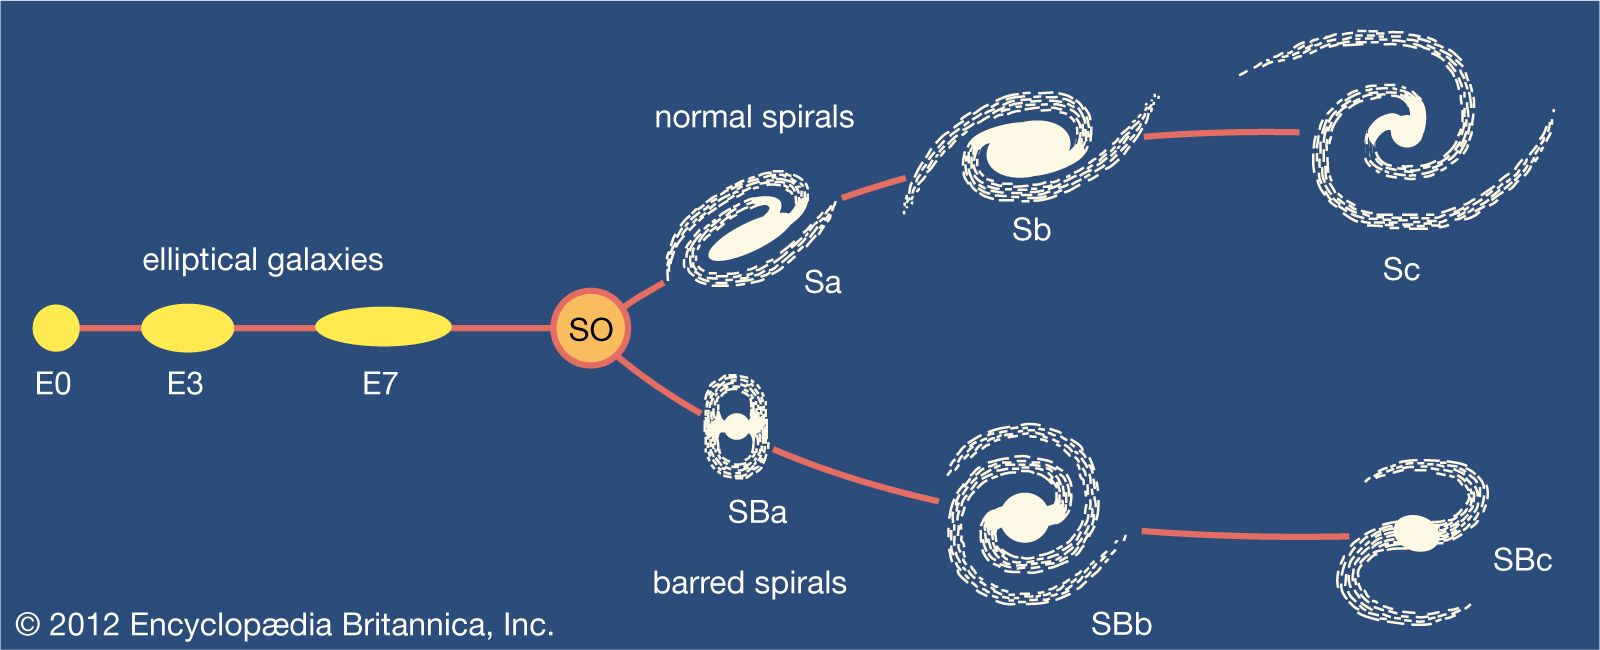
\includegraphics[width=12cm]{figures/figure1_15.jpg}
\captionsetup{justification=raggedright, singlelinecheck=false}
\caption{哈勃音叉图 (Hubble Tuning Fork Scheme).}
\label{哈勃音叉图。}
\end{figure}

和恒星能组成星团一样,星系也能组成星系群和星系团,前者一般包含数十个星系,后者成员数目可以上千。星系团中椭圆星系占主导地位,核心区主要是 E, S0 等早型星系,S 多处于星系团外围。星系群中则是漩涡星系主导。

星系分布的不均匀不仅体现在成团性上。观测数千个星系光谱以确定距离和位置,发现宇宙主要由纤维和巨洞 (voids) 组成,大部分物质处于纤维结构上,约占整个空间体积 1\%。巨洞典型大小$50\,\mathrm{Mpc}$.

接下来我们将介绍各类型星系的特征,并解释一下图\ref{哈勃音叉图。}所呈现出的信息。

\subsubsection{不同类型的星系特征}

\paragraph{椭圆星系}~{}

记长轴为$a$,短轴为$b$,可将椭圆星系按椭率大小分为 E0 到 E7 八个次型:
\begin{equation}
n=\frac{10\left(a-b\right)}{a}.
\end{equation}

椭圆星系没有星系盘、颜色偏红,星系中心最亮,亮度向边缘递减。椭圆星系主要由年老恒星和大量热气体组成,没有或仅有少量的冷气体和尘埃。椭圆星系的特征为强吸收线,少有发射线,因为年老的低光度恒星成员大气中有很多金属。普通椭圆星系光度为银河系数倍,特征尺度为数十个$\mathrm{kpc}$.

一种特殊的椭圆星系记作 cD, c 表示星系非常大,D 表示星系外观非常弥散,这种星系称作巨椭圆星系,通常为星系团中最明亮的星系,比银河系亮 100 倍以上,巨大弥散包层可延伸到数百$\mathrm{kpc}$,质量可达$10^{13}M_{\odot}$. cD 多位于星系团中心,可能诞生自星系团中最亮的星系吞噬次亮星系,弥散包层(星系晕)可能为次亮星系的遗迹。这个推断并非空穴来风,实际上普通椭圆星系也有子结构。10\%\text{\textendash}20\%的椭圆星系外区有弧状壳和其他不对称的结构,应当是被大星系引力撕碎并捕获的小星系遗迹(这个过程是星系并合的一种),壳层是星系吸积过程的直接证据。

除了普通椭圆星系和 cD,还有暗椭圆星系。暗椭圆星系光度不足银河系光度十分之一,分为致密的矮椭圆星系 (dE)、暗弱的弥散矮椭圆星系和更暗的矮椭球星系 (dSph).多数矮星系内部有球状星团存在。dE 是小的椭圆星系,质量可能只有$10^{7}M_{\odot}$,但属性与一般的椭圆星系差别较大。dSph 本质和 dE 可能并无区别,但面亮度更低,光度甚至接近球状星团,因此大部分是我们无法观测到的。dSph 内部几乎没有年轻的恒星(只有 2\%的恒星年龄小于 25 亿年),主要由老年、中年恒星组成(诞生于宇宙年龄$3/7/15\,\mathrm{Gyr}$的三次暴发),说明 dSph 的形成时间很早。dSph 尘埃、气体很少,易受到主星系的引力作用从而碎裂、瓦解。dSph 中有大量暗物质,而球状星团中还没有探测到暗物质。

椭圆星系的光度决定了椭圆星系的很多特性。亮椭圆星系中恒星运动以随机(谈轨道随机主要指角速度方向随机,不会像银河系那样基本都指向北银极)的椭圆轨道运动为主,朝向统一方向的旋转运动少。反过来讲,较暗椭圆星系有较多的旋转运动,随机运动较小。dE 和 dSph 旋转和随机运动的相对重要性无明显规律。此外,一般来讲星系越暗,金属丰度越低。所有的 dSph 重元素丰度低,最亮的 dSph 金属丰度也不过太阳的$\dfrac{1}{30}$.原因在于这些星系恒星形成困难,难以通过热核反应生成重元素,同时引力较弱,即使生成了,由于主序阶段结束时剧烈的质量抛射,金属增丰的气体也容易脱离星系束缚来到星系际空间。

\paragraph{漩涡星系和棒旋星系}~{}

漩涡星系具有核球、棒/环、盘、旋臂和晕。分类主要看核球大小和旋臂缠绕程度。如图\ref{哈勃音叉图。}所示,Sa 核球最大,旋臂紧卷,Sc 核球成为一个小亮核,旋臂松弛。从 Sa 到 Sc,年轻恒星和气体的比例不断增加。从 Sa 到 Sd,星系光度逐渐变小,中心面亮度逐渐变小,颜色逐渐变蓝,星系中中性氢气体比例逐渐增加。

漩涡星系光谱特征为强发射线,因为有年轻恒星加热周围的气体。同时有吸收特征,来自年老星族。一般来讲漩涡星系星系盘颜色偏蓝,星系晕和核球偏红,也说明有星族差异。

棒由恒星组成,棒结构贯穿核心部分。一半以上的漩涡星系中有棒,可能起源于引力不稳定性。SB 分类判据与 S 类似,从左往右棒逐渐变弱,旋臂逐渐松散。旋臂起源于棒的两端。

\paragraph{不规则星系}~{}

不规则星系中包括星暴星系、并合星系等恒星形成星系,富含星际气体、尘埃和年轻恒星,因此其光谱中也有强大的发射线,来自年轻恒星和周围的电离氢区。

不规则星系可分为 Irr\uppercase\expandafter{\romannumeral 1}和 Irr\uppercase\expandafter{\romannumeral 2}类。前者有隐约可见的旋涡结构,后者无定形外貌,可能是正在爆发或爆发后的星系,或者是受伴星系引力扰动而扭曲了的星系。

小的不规则星系称为矮不规则星系,内部以年轻星族为主、气体含量多,质量不大$(<10^{10}M_{\odot})$.与矮椭球星系的不同之处是它们有气体和年轻蓝星,因此矮椭球星系很可能是失去或用尽了气体的矮不规则星系。

\paragraph{总结}~{}

早型星系 (E, S0) 高光度,红色,年轻恒星比例少。

晚型星系 (S, Irr) 低光度,蓝色,有占比较高的新诞生的大质量恒星。

尽管 S 和 Irr 数目众多,E 却包含了恒星总质量的大约一半。

近邻星系样本中,大约有 70\%的 S,30\%的 E 和 3\%的 Irr.如此样本分布可能要考虑光度引起的选择效应(如果观测表明暗弱的星系比较少,不代表实际上真的比较少,可能是仪器没法发现)。

\begin{table}[htbp]
\centering
\caption{分类小结}
\begin{tabular}{c c c c}
\hline
 & 漩涡/棒旋星系 & 椭圆星系 & 不规则星系\\
\cline{1-4}
\textbf{形态} & 由恒星和气体构成的盘和星系晕 & 球形或椭圆形 & 无明显结构\\
 & 棒旋星系的核心有棒状结构 & 可能有子结构 & 可能有隐约漩涡结构\\
\cline{1-4}
\textbf{星族} & 盘包含年轻和年老的恒星 & 光度和质量基本上 & 包含年轻和年老的恒星\\
 & 晕只有年老的恒星 & 都由年老的恒星主导 & \\
\cline{1-4}
\textbf{星际介质} & 盘包含大量气体和尘埃 & 没有或只有很少的气体和尘埃 & 富含气体和尘埃\\
 & 晕中的气体和尘埃很少 &  & \\
\cline{1-4}
\textbf{恒星形成} & 旋臂中有恒星形成过程 & 近几十亿年没有明显恒星形成 & 强烈的恒星形成过程\\
\cline{1-4}
 & 盘中的恒星和气体 & 恒星绕星系核心 & 恒星和气体成分\\
\textbf{天体运动} & 绕核心作圆轨道运动 & 作随机轨道运动 & 具有较显著的无规则运动\\
 & 晕中的恒星绕核心作随机运动 & 质量越低旋转运动越多 & \\
\cline{1-4}
\end{tabular}
\label{2}
\end{table}

\subsubsection{星系测光}
星系的形态分类是定性描述,甚至比较依靠目视分类(当然现在也有用机器学习做的),要定量描述我们需要测光。对于点源,我们可以在成像平面上画一个孔径(不一定是圆形)将恒星圈住,积分孔径内的星等进行测光。对于星系也可以这么做,但是星系外围的亮度可能天光背景还暗,很难确定星系大小和形状,也就不知该如何选择孔径。既然如此,不妨就将光度刚好低至某一值的边界作为星系半径。为此,我们先要引入二维面亮度分布的概念,以此描述星系图像上某一特定区域在某一波段内的光度。记该区域物理边长为$D$,光度为$L$,星系到我们的距离为$d$,可以定义:
\begin{equation}
I\left(x\right)=\frac{F}{\theta^{2}}=\dfrac{\dfrac{L}{4\pi{}d^{2}}}{\dfrac{D^{2}}{d^{2}}}=\frac{L}{4\pi{}D^{2}}.\label{1.5.2}
\end{equation}
可以发现面亮度不依赖于星系的距离。(但实际上并非如此,我们会在宇宙学一节说明这一点。)

自 (\ref{1.5.2}) 式出发,我们发现星系某一点处的面亮度有两种表示方法,一种是$I\left(x\right)=m\,\mathrm{mag\cdot arcsec^{-2}}$,即单位平方角秒的星等,用于孔径测光很方便。但星等涉及到距离,有时我们更关心星系的本征性质,因此需要用$L_{\odot}\cdot\mathrm{pc^{-2}}$作为单位。记太阳绝对星等为$M_{\odot}$,星系距离$d\,\mathrm{pc}$,第二种表示法与第一种表示法的关系为:
\begin{align}
m-M_{\odot}&=-2.5\log_{10}\left(\frac{\dfrac{L}{4\pi\left(d\,\mathrm{pc}\right)^{2}}}{\dfrac{L_{\odot}}{4\pi\left(10\,\mathrm{pc}\right)^{2}}}\right),\notag\\
L&=L_{\odot}\times10^{-\frac{m-M_{\odot}}{2.5}-2}\times d^{2},\notag\\
I\left(R\right)&=\frac{L}{\left(d\,\mathrm{pc}\times1^{\prime\prime}\right)^{2}}=\left(\frac{64800}{\pi}\right)^{2}\frac{L}{\left(d\,\mathrm{pc}\right)^{2}}=\left(\frac{64800}{\pi}\right)^{2}\times10^{-\frac{m-M_{\odot}}{2.5}-2}L_{\odot}\cdot\mathrm{pc}^{-2}.
\end{align}

确立了描述光度的方法,就可以确定边界了。首先定义等照度线,它是星系图像上面亮度相等的像源的连线。通常取 B 波段$I_{\text{B}}(x)=25\,\mathrm{mag\cdot arcsec^{-2}}$的等照度线作为星系边界,对应的半径记为$R_{25}$.或者取霍姆伯格半径$I_{\text{B}}(x)=26.5\,\mathrm{mag\cdot arcsec^{-2}}$.

有一类星系被称作 Low Surface Brightness Galaxy (LSBGs),它们中心区域$I_{\text{B}}$低于$23\,\mathrm{mag\cdot arcsec^{-2}}$.多数 LSBGs 为矮星系。转动曲线显示质量光度比较大,可能的原因包括:暗物质比例大;平均气体密度小,恒星形成效率低,重子物质主要以气体而非恒星形式存在。

\subsection{宇宙学基础}
宇宙学可能是本章节最有趣的部分,但是绪论部分已经特别长了,所以本节就简单推导一下用来描述宇宙的 Friedmann 方程,填一下宇宙学红移的坑并介绍一下宇宙历史吧。

\subsubsection{Friedmann 方程}
1920 年代,哈勃在测定星系光谱时发现,星系光谱都有一定程度的红移,且距离我们越远,退行速度越快,即哈勃定律
\begin{equation}
v=H_{0}\cdot D,
\end{equation}
其中$H_{0}$被称作哈勃常数,大约$70\,\mathrm{km\cdot{}s^{-1}\cdot Mpc^{-1}}$.习惯上还会引入一个参数$h$,它是哈勃常数数值的百分之一,和普朗克常数并没有什么关系。

即然星系都在离我们远去,一个自然的想法是进行时间反演,那是不是说明宇宙的最初所有物质都集中在一点?如果空间无限大而只有物质集中似乎也不是一个很合理图景,那有没有可能空间最初也集中在一点,只是随着时间不断膨胀。如同一根不断拉伸的橡皮筋,物质则是橡皮筋上的刻度,如此便解释了哈勃定律的线性关系。

为更好地理解宇宙的膨胀,我们可以将时空想象成一张方格纸,在神秘力量的作用下,方格纸在不断变大,也就是物理坐标在变化。但如果我们以格点数为坐标,那么物质在格点坐标系的坐标并没有变化。于是我们可以定义随时间变化无量纲的尺度因子$a\left(t\right)$.将格点坐标系称为共动 (comoving) 坐标系,实际物理空间中的距离,等于尺度因子乘共动坐标系中的距离。这样子可以解释哈勃定律并给出哈勃常数:
\begin{align}
v=\frac{\mathrm{d}r}{\mathrm{d}t}=\frac{\mathrm{d}a}{\mathrm{d}t}x=\dot{a}\frac{ax}{a}=Hr,H\left(t\right)=\frac{\dot a\left(t\right)}{a\left(t\right)}.
\end{align}

除了尺寸,方格纸的弯曲程度(度规)也是我们关心的部分。我们很自然期望物质分布对称一点这样度规也对称一点。人们在观测中提出了宇宙学原理:宇宙大尺度上是均匀和各向同性的。前者意味着处处一样,后者意味着朝各个方向看都是一样的。如此便要求空间具有最大对称性,可以推导出这个度规的形式为
\begin{equation}
\mathrm{d}s^{2}=c^{2}\mathrm{d}t^{2}-a^{2}\left(t\right)\left(\mathrm{d}r^{2}+S_{k}^{2}\left(r\right)\mathrm{d}\Omega^{2}\right),\quad S_{k}\left(r\right)=
\begin{cases}
\sin r,&k=1,\\
r,&k=0,\\
\sinh r,&k=-1.
\end{cases}
\end{equation}
或者改写成更方便计算的形式:
\begin{equation}
\mathrm{d}s^{2}=-\mathrm{d}t^{2}+a^{2}\left(t\right)\left\{\frac{\mathrm{d}r^{2}}{1-kr^{2}}+r^{2}\left(\mathrm{d}\theta^{2}+\sin^{2}\theta\mathrm{d}\phi^{2}\right)\right\}.\label{1.6.4}
\end{equation}
$k=1$是封闭的球面,$k=0$是平直宇宙,$k=-1$是开放双曲宇宙。

爱因斯坦场方程告诉我们物质是如何影响时空膨胀的,我们可以从 (\ref{1.6.4}) 式出发一步步推导。首先列出不为零的度规各分量和度规分量对坐标分量的导数:
\begin{align}
g_{00}&=-1,\notag\\
g_{11}&=\frac{a\left(t\right)^{2}}{1-kr^{2}},\frac{\partial{}g_{11}}{\partial{}x^{0}}=2\frac{\dot a}{a}g_{11},\frac{\partial{}g_{11}}{\partial{}x^{1}}=\frac{2k}{1-kr^{2}}g_{11},\notag\\
g_{22}&=a\left(t\right)^{2}r^{2},\frac{\partial{}g_{22}}{\partial{}x^{0}}=2\frac{\dot a}{a}g_{22},\frac{\partial{}g_{22}}{\partial{}x^{1}}=\frac{2g_{22}}{r},\notag\\
g_{33}&=a\left(t\right)^{2}r^{2}\sin^{2}\theta,\frac{\partial{}g_{33}}{\partial{}x^{0}}=2\frac{\dot a}{a}g_{33},\frac{\partial{}g_{33}}{\partial{}x^{1}}=\frac{2g_{33}}{r},\frac{\partial{}g_{33}}{\partial{}x^{2}}=\frac{2g_{33}\cos\theta}{\sin\theta}.\notag
\end{align}
接着根据
\begin{equation}
\Gamma_{\alpha\beta}^\mu=\frac{g^{\mu\nu}}{2}\left[g_{\alpha\nu,\beta}+g_{\beta\nu,\alpha}-g_{\alpha\beta,\nu}\right]
\end{equation}
计算克氏符:
\begin{align}
\Gamma_{\alpha\beta}^0&=\frac{g^{00}}{2}\left[g_{\alpha0,\beta}+g_{\beta0,\alpha}-g_{\alpha\beta,0}\right]=-\frac{g^{00}}{2}\frac{\partial{}g_{\alpha\beta}}{\partial{}t}\delta_{\alpha\beta}=g_{\alpha\beta}\frac{\dot a}{a}\delta_{\alpha\beta},\,\text{when}\,\alpha,\beta>0.\notag\\
\Gamma_{0\beta}^\mu&=\frac{g^{\mu\mu}}{2}\left[g_{0\mu,\beta}+g_{\beta\mu,0}-g_{0\beta,\mu}\right]=\frac{g^{\mu\mu}}{2}\frac{\partial{}g_{\beta\mu}}{\partial{}t}\delta_{\beta\mu}=\frac{\dot a}{a}\delta_{\beta\mu},\,\text{when}\,\mu,\beta>0.\notag\\
\Gamma_{\alpha\beta}^1&=\frac{g^{11}}{2}\left[g_{\alpha1,\beta}+g_{\beta1,\alpha}-g_{\alpha\beta,1}\right],\notag\\
\Gamma_{11}^{1}&=\frac{g^{11}}{2}\frac{\partial{}g_{11}}{\partial{}r},\Gamma_{22}^{1}=-\frac{g^{11}}{2}\frac{\partial{}g_{22}}{\partial{}r},\Gamma_{33}^{1}=-\frac{g^{11}}{2}\frac{\partial{}g_{33}}{\partial{}r}.\notag\\
\Gamma_{\alpha\beta}^{2}&=\frac{g^{22}}{2}\left[\frac{\partial{}g_{\alpha2}}{\partial{}x^\beta}+\frac{\partial{}g_{\beta2}}{\partial{}x^\alpha}-\frac{\partial{}g_{\alpha\beta}}{\partial{}\theta}\right],\notag\\
\Gamma_{12}^{2}&=\Gamma_{21}^{2}=\frac{1}{r},\Gamma_{33}^{2}=-\sin\theta\cos\theta.\notag\\
\Gamma_{\alpha\beta}^{3}&=\frac{g^{33}}{2}\left[\frac{\partial{}g_{\alpha3}}{\partial{}x^\beta}+\frac{\partial{}g_{\beta3}}{\partial{}x^\alpha}\right],\notag\\
\Gamma_{13}^{3}&=\Gamma_{31}^{3}=\frac{1}{r},\Gamma_{23}^{3}=\Gamma_{32}^{3}=\frac{\cos\theta}{\sin\theta}.\notag
\end{align}
我们不难发现只有 19 项不为 0,
\begin{align}
\Gamma_{11}^{0}&=\frac{a\left(t\right)\dot{a}\left(t\right)}{1-kr^{2}},\Gamma_{22}^{0}=a\left(t\right)\dot{a}\left(t\right)r^{2},\Gamma_{33}^{0}=a\left(t\right)\dot{a}\left(t\right)r^{2}\sin^{2}\theta,\notag\\
\Gamma_{10}^{1}&=\Gamma_{01}^{1}=\frac{\dot a}{a},\Gamma_{11}^{1}=\frac{kr}{1-kr^{2}},\notag\\
\Gamma_{22}^{1}&=-r\left(1-kr^{2}\right),\Gamma_{33}^{1}=-r\left(1-kr^{2}\right)\sin^{2}\theta,\notag\\
\Gamma_{20}^{2}&=\Gamma_{02}^{2}=\frac{\dot a}{a},\Gamma_{12}^{2}=\Gamma_{21}^{2}=\frac{1}{r},\Gamma_{33}^{2}=-\sin\theta\cos\theta,\notag\\
\Gamma_{30}^{3}&=\Gamma_{03}^{3}=\frac{\dot a}{a},\Gamma_{13}^{3}=\Gamma_{31}^{3}=\frac{1}{r},\Gamma_{23}^{3}=\Gamma_{32}^{3}=\frac{\cos\theta}{\sin\theta}.\notag
\end{align}
进而可根据
\begin{equation}
R_{\mu\nu}=\Gamma_{\mu\nu,\alpha}^{\alpha}-\Gamma_{\mu\alpha,\nu}^{\alpha}+\Gamma_{\beta\alpha}^{\alpha}\Gamma_{\mu\nu}^{\beta}-\Gamma_{\beta\nu}^{\alpha}\Gamma_{\mu\alpha}^{\beta}
\end{equation}
计算 Ricci 张量:
\begin{align}
R_{00}&=\Gamma_{00,\alpha}^{\alpha}-\Gamma_{0\alpha,0}^{\alpha}+\Gamma_{\beta\alpha}^{\alpha}\Gamma_{00}^{\beta}-\Gamma_{\beta0}^{\alpha}\Gamma_{0\alpha}^{\beta}=-\frac{\partial{}\Gamma_{01}^{1}}{\partial{}t}-\frac{\partial{}\Gamma_{02}^{2}}{\partial{}t}-\frac{\partial{}\Gamma_{03}^{3}}{\partial{}t}-\left(\frac{g^{ii}}{2}\frac{\partial{}g_{ii}}{\partial{}t}\right)^{2}\notag\\
&=-3\frac{\mathrm{d}}{\mathrm{d}t}\left(\frac{\dot{a}\left(t\right)}{a\left(t\right)}\right)-3\left(\frac{\dot{a}\left(t\right)}{a\left(t\right)}\right)^{2}=-3\frac{\ddot{a}}{a}.\notag\\
R_{11}&=\left[\frac{\partial{}\Gamma_{11}^{0}}{\partial{}t}\right]-\left[\frac{\partial{}\Gamma_{12}^{2}}{\partial{}r}+\frac{\partial{}\Gamma_{13}^{3}}{\partial{}r}\right]+\left[\Gamma_{11}^{0}\left(\Gamma_{01}^{1}+\Gamma_{02}^{2}+\Gamma_{03}^{3}\right)+\Gamma_{11}^{1}\left(\Gamma_{11}^{1}+\Gamma_{12}^{2}+\Gamma_{13}^{3}\right)\right]\notag\\
&\quad-\left[2\Gamma_{10}^{1}\Gamma_{11}^{0}+\Gamma_{11}^{1}\Gamma_{11}^{1}+\Gamma_{12}^{2}\Gamma_{21}^{2}+\Gamma_{13}^{3}\Gamma_{31}^{3}\right]\notag\\
&=\frac{a^{2}}{1-kr^{2}}\left(\frac{\ddot a}{a}+2\left(\frac{\dot{a}}{a}\right)^{2}+\frac{2k}{a^{2}}\right).\notag\\
R_{22}&=\left[\frac{\partial{}\Gamma_{22}^{0}}{\partial{}t}+\frac{\partial{}\Gamma_{22}^{1}}{\partial{}r}\right]-\left[\frac{\partial{}\Gamma_{23}^{3}}{\partial{}\theta}\right]+\left[\Gamma_{22}^{0}\Gamma_{0\alpha}^{\alpha}+\Gamma_{22}^{1}\Gamma_{1\alpha}^{\alpha}\right]-\left[\Gamma_{22}^{0}\Gamma_{20}^{2}+\Gamma_{22}^{1}\Gamma_{21}^{2}+\Gamma_{02}^{2}\Gamma_{22}^{0}+\Gamma_{12}^{2}\Gamma_{22}^{1}+\Gamma_{32}^{3}\Gamma_{23}^{3}\right]\notag\\
&=a^{2}r^{2}\left(\frac{\ddot{a}}{a}+2\left(\frac{\dot{a}}{a}\right)^{2}+\frac{2k}{a^{2}}\right).\notag\\
R_{33}&=\left[\frac{\partial{}\Gamma_{33}^{0}}{\partial{}t}+\frac{\partial{}\Gamma_{33}^{1}}{\partial{}r}+\frac{\partial{}\Gamma_{33}^{2}}{\partial{}\theta}\right]-\left[0\right]+\left[\Gamma_{33}^{0}\Gamma_{0\alpha}^{\alpha}+\Gamma_{33}^{1}\Gamma_{1\alpha}^{\alpha}+\Gamma_{33}^{2}\Gamma_{2\alpha}^{\alpha}\right]\notag\\
&\quad-\left[\Gamma_{33}^{0}\Gamma_{30}^{3}+\Gamma_{33}^{1}\Gamma_{31}^{3}+\Gamma_{33}^{2}\Gamma_{32}^{3}+\Gamma_{03}^{3}\Gamma_{33}^{0}+\Gamma_{13}^{3}\Gamma_{33}^{1}+\Gamma_{23}^{3}\Gamma_{33}^{2}\right]\notag\\
&=a^{2}r^{2}\sin^{2}\theta\left(\frac{\ddot a}{a}+2\left(\frac{\dot a}{a}\right)^{2}+\frac{2k}{a^{2}}\right).\notag
\end{align}
幸运的是,其他几项很容易算
\begin{align}
R_{10}&=0-0+\Gamma_{10}^{1}\Gamma_{1\alpha}^{\alpha}-\Gamma_{\alpha0}^{\alpha}\Gamma_{1\alpha}^{\alpha}=0.\notag\\
R_{20}&=0-0+\Gamma_{20}^{2}\Gamma_{2\alpha}^{\alpha}-\Gamma_{30}^{3}\Gamma_{23}^{3}=0.\notag\\
R_{30}&=0.\notag\\
R_{12}&=0-0+\Gamma_{12}^{2}\Gamma_{2\alpha}^{\alpha}-\Gamma_{32}^{3}\Gamma_{13}^{3}=0.\notag\\
R_{13}&=0.\notag\\
R_{23}&=0.\notag
\end{align}
于是我们成功得到了 Ricci 标量
\begin{align}
R&=g^{\mu\nu}R_{\mu\nu}=3\frac{\ddot a}{a}+\left[\frac{\ddot a}{a}+2\left(\frac{\dot a}{a}\right)^{2}+\frac{2k}{a^{2}}\right]\times3\notag\\
&=6\left[\frac{\ddot a}{a}+\left(\frac{\dot a}{a}\right)^{2}+\frac{k}{a^{2}}\right].\notag
\end{align}
均匀宇宙中物质是理想流体,能动张量为$T^{\mu}_{\nu}=\begin{pmatrix}
\rho & 0 & 0 & 0\\
0 & P & 0 & 0\\
0 & 0 & P & 0\\
0 & 0 & 0 & P
\end{pmatrix}$,考虑爱因斯坦场方程的 00 分量
\begin{equation}
G_{00}=R_{00}-\frac{1}{2}g_{00}R=8\pi\mathrm{G}\rho=3\left[\left(\frac{\dot a}{a}\right)^{2}+\frac{k}{a^{2}}\right].\notag
\end{equation}
改写一下就是 the first Friedmann equation
\begin{equation}
H^{2}\left(t\right)=\left(\frac{\dot{a}\left(t\right)}{a\left(t\right)}\right)^{2}=\frac{8\pi\mathrm{G}}{3}\rho\left(t\right)-\frac{k}{a^{2}\left(t\right)}.
\end{equation}
当然还可以在场方程中添加一项宇宙学常数(暗能量),方程变为
\begin{equation}
\left(\frac{\dot{a}\left(t\right)}{a\left(t\right)}\right)^{2}=\frac{8\pi\mathrm{G}}{3}\rho\left(t\right)-\frac{k}{a^{2}\left(t\right)}+\frac{\Lambda}{3}.\label{1.6.8}
\end{equation}
于是我们发现决定宇宙膨胀速率的要素有物质密度$\rho$,曲率$k$,还有暗能量$\Lambda$.如果要让现在的宇宙继续维持平坦(即$k=0$)且不考虑暗能量,密度就需要达到
\begin{equation}
\rho_{\text{cri}\left(t\right)}=\frac{3H_{0}^{2}\left(t\right)}{8\pi\mathrm{G}}\sim1.88\times10^{-29}h^{2}\,\mathrm{g\cdot{}cm^{-3}}.
\end{equation}
这就是临界密度的表达式。

考虑场方程其他分量我们还能得到
\begin{equation}
\left(\frac{\dot{a}}{a}\right)^{2}+\frac{k}{a^{2}}+2\frac{\ddot{a}}{a}=-8\pi\mathrm{G}P.\\
\end{equation}
同样考虑暗能量,得到 the second Friedmann equation
\begin{equation}
\frac{\ddot{a}}{a}=-\frac{4\pi\mathrm{G}}{3}\left(\rho\left(t\right)+3P\left(t\right)\right)+\frac{\Lambda}{3}.\label{1.6.10}
\end{equation}
可见决定宇宙膨胀加速度的要素有物质的能动张量和暗能量。

\subsubsection{物态方程}
(\ref{1.6.8}) 式对时间求导代入 (\ref{1.6.10}) 式得到连续性方程
\begin{equation}
\dot{\rho}+3\frac{\dot{a}}{a}\left(\rho\left(t\right)+P\left(t\right)\right)=0.
\end{equation}
一般情况下我们假设宇宙学常数和曲率都不随时间变化,此时有三个未知数$\rho,P,a$但只有两个独立方程,为此要给出物质的状态方程
\begin{equation}
P=\omega\rho.
\end{equation}
代入上式可以发现
\begin{equation}
\rho\propto{}a^{-3\left(1+\omega\right)}.
\end{equation}

单论宇宙中的物质,可以分为非相对论性物质和相对论性物质两类。前者密度自然和体积成反比,即$\rho_{\text{matter}}\propto a^{-3}$,另外由于其分布较为松散且相互作用弱(宇宙是超真空),可以认为$P_{\text{m}}=0,\omega=0$.而对于相对论性物质,我们曾经推导过辐射压和能量密度的关系,因此$\omega=\dfrac{1}{3}$.由于$\rho_{\text{radiation}}\propto{}T^{4}$,而光子气体绝热过程熵$S\propto{}T^{3}V$不变,故$\rho_{\text{raditation}}\propto{}a^{-4}$.也可从这个角度理解:在体积增长的前提下,光子的波长也因为空间的拉伸变长了。什么你说这样子能量不守恒,那确实是这样的……对于暗能量,我们一般认为它满足$\omega=-1$.此时发现暗能量的能量密度始终不变,那么随着宇宙体积增加宇宙总能量居然在上升!当然最近的观测结果表明$\omega$对$-1$有一定偏离,甚至宇宙学常数可能不是常数,在随时间变化。

有了不同物质的物态方程,我们便可以解出$a$随时间的变化了。假如宇宙中只有非相对论物质且$k=0$,那么
\begin{equation}
\left(\frac{\dot{a}}{a}\right)^{2}\propto{}a^{-3},a\propto{}t^{2/3},H=\frac{\dot{a}}{a}=\frac{2}{3t},
\end{equation}
于是可以用哈勃常数推断宇宙年龄。如果平坦宇宙中只有辐射,那么
\begin{equation}
a\propto{}t^{1/2},H=\frac{1}{2t}.
\end{equation}
暗能量主导时宇宙指数膨胀
\begin{equation}
a=e^{Ht},H=\sqrt{\frac{8\pi\mathrm{G}\rho_{\Lambda}}{3}}.
\end{equation}
最后,(\ref{1.6.8}) 式两侧同除现在的哈勃常数$H_{0}^{2}$可以得到无量纲形式,更方便地展示各组分的贡献
\begin{equation}
H^{2}\left(t\right)=H_{0}^{2}\left[\Omega_{\text{r,0}}\left(\frac{a_{0}}{a\left(t\right)}\right)^{4}+\Omega_{\text{m,0}}\left(\frac{a_{0}}{a\left(t\right)}\right)^{3}+\Omega_{\text{k,0}}\left(\frac{a_{0}}{a\left(t\right)}\right)^{2}+\Omega_{\Lambda}\right].
\end{equation}

\subsubsection{宇宙学红移}
既然宇宙在膨胀,光子波长会被拉伸,那么波长和$a$到底有什么关系呢?或许现在我们就可以聊聊宇宙学红移了。对于光子,它所走过的世界线始终为 0,取$k=0,\mathrm{d}\theta=0,\mathrm{d}\phi=0$,可得
\begin{equation}
\mathrm{d}s^{2}=-\mathrm{d}t^{2}+a^{2}\left(t\right)\mathrm{d}r^{2}=0.
\end{equation}
计算光子走过的空间距离得到
\begin{equation}
\chi=\int_{r_{1}}^{r_{2}}\mathrm{d}r=\int_{t_{1}}^{t_{2}}\frac{\mathrm{d}t}{a\left(t\right)}.
\end{equation}
假设辐射源处电矢量在$t_{1}$时刻达到峰值,$t_{2}$时刻为我们所接收,源处经过$\Delta{}t_{1}$又达到峰值,$t_{2}+\Delta{}t_{2}$接收,由于光子走过距离一致,很自然有
\begin{equation}
\int_{t_{1}}^{t_{2}}\frac{\mathrm{d}t}{a\left(t\right)}=\int_{t_{1}+\Delta{}t_{1}}^{t_{2}+\Delta{}t_{2}}\frac{\mathrm{d}t}{a\left(t\right)}.
\end{equation}
因此变化的积分限给予的贡献是一致的:
\begin{equation}
\frac{\Delta{}t_{2}}{a\left(t_{2}\right)}=\frac{\Delta{}t_{1}}{a\left(t_{1}\right)}.
\end{equation}
时间间隔比就是波长比,于是得到
\begin{equation}
\frac{\lambda_{2}}{\lambda_{1}}=\frac{a_{2}}{a_{1}}.
\end{equation}
记如今的尺度因子为$a_{0}=1$,宇宙早期尺度因子为$a$,我们得到宇宙学红移表达式
\begin{equation}
z=\frac{a_{0}}{a}-1=\frac{1}{a}-1.
\end{equation}
举个例子,当我们在说红移$z=1$时,$a=\dfrac12$,那时候宇宙只有现在一半大(半径)。

\subsubsection{特殊的距离}
我们刚才介绍了光子的距离,它也被称作共动距离。我们已经知道了尺度因子、哈勃常数、红移之间的关系,因此它也可以改写成
\begin{equation}
\chi\left(a\right)=\int_{t\left(a\right)}^{t_0}\frac{\mathrm{d}t'}{a\left(t'\right)}=\int_{a}^{a_{0}}\frac{\mathrm{d}a'}{a'^{2}H\left(a'\right)}=\int\frac{\mathrm{d}a'}{\mathrm{d}z'}\frac{\mathrm{d}z'}{a'^{2}H'}=-\int_{z}^{0}\frac{\mathrm{d}z}{H\left(z\right)}.
\end{equation}

现在我们考虑我们所见到的天体的角尺寸。在实际宇宙距离中,考虑到光一边传播宇宙一边膨胀,实际上很难计算。我们可以在 comoving 坐标系中考虑这个问题。天体到我们的距离就是$\chi\left(a\right)$,物理直径为$l$的天体在红移$z$处在 comoving 坐标系中的大小是$l/a$,那么角度很明显就是
\begin{equation}
\theta=\frac{l/a}{\chi}.
\end{equation}
那么我们可以定义角直径距离
\begin{equation}
d_{\theta}=\frac{l}{\theta}=a\chi=\frac{\chi}{1+z}.
\end{equation}

在一个平坦的物质主导的$\Omega=1$的宇宙中,
\begin{align}
a\left(t\right)&=a_{0}\left(\frac32H_{0}t\right)^{\frac23}.\notag\\
H\left(z\right)&=\frac{\dot a}{a}=\frac{2}{3t}=H_{0}\left(1+z\right)^{\frac32}.\notag\\
\chi&=\frac{c}{H_{0}}\int_{0}^{z}\left(1+z\right)^{-\frac32}\mathrm{d}z=\frac{2c}{H_{0}}\left(1-\left(1+z\right)^{-\frac12}\right).\notag\\
\theta&=\frac{l}{\chi}\left(1+z\right)=\frac{lH_{0}}{2c}\frac{1+z}{1-\left(1+z\right)^{-\frac12}}.
\end{align}
于是我们发现,天体的角直径随红移增加先下降后上升,高红移处天体看起来反而更大了。

另一个要定义的距离则是光度距离。我们所接收到的光度为
\begin{equation}
F=\frac{L(\chi)}{4\pi \chi^2(a)}.
\end{equation}
因为宇宙膨胀,光子能量降低,同时视线方向单位长度包含的光子数少了,故$L\left(\chi\right)=La^{2}$,光度距离
\begin{equation}
d_{L}=\left(\frac{L}{4\pi F}\right)^{\frac12}=\chi\left(1+z\right).
\end{equation}
此时天体面亮度
\begin{equation}
I(x)=\frac{F}{\theta^{2}}=\frac{L/(4\pi d_{L}^{2})}{D^{2}/d_{\theta}^{2}}=\frac{L}{4\pi D^{2}}\frac{1}{\left(1+z\right)^{4}},
\end{equation}
不再是常数,而是随着红移增加快速下降,因此高红移天体非常暗。

\subsubsection{宇宙历史}
最后我们简单介绍一下宇宙历史。首先是大爆炸,宇宙诞生。$0\text{\textendash}10^{-43}\,\mathrm{s}$被称作普朗克时期,此时$T\sim10^{32}\,\mathrm{K}$,宇宙半径$\sim0.01\,\mathrm{cm}$,四大作用力基本统一。我们认为宇宙中存在一种特殊的场(真空能),它可以推动空间随时间的指数膨胀,按半径算的话,宇宙至少膨胀了$10^{25}$,由于真空能能量密度不变,总能量至少翻了$10^{75}$,这个过程被称作暴胀 (Inflation).暴胀大概在宇宙年龄$10^{-30}\,\mathrm{s}$就结束了。

接下来暴胀场的能量会转移到标准模型粒子中,此时物质都是相对论性的基本粒子和其反粒子,能量等于温度,所以宇宙变得高热,充满了可以把任何原子核粉碎为其组成粒子的高能光子。此时光子和粒子数目大致相等。但值得注意的是,如今的宇宙几乎没有反物质,因此这些粒子含量其实是不对称的。

随着宇宙膨胀温度下降,重子和反重子大量湮灭(温度降低无法进行逆过程),留下大量轻子(光子、正负电子、正负$\mu$介子,中微子以及少数核子)。此时电子、光子、中微子耦合在一起(持续相互碰撞,相互产生)。宇宙一片黑暗。

等到宇宙诞生$1\,\mathrm{s}$时,由于温度进一步降低,中微子退耦了,散射了出去,形成了中微子背景。不过实际上尚未观测到。

第三分钟,随着温度进一步下降 ($10^{9}\,\mathrm{K}$),粒子动能不足以撞散原子核,质子和中子开始结合成氢、氦等元素。等宇宙膨胀速率大于质子中子碰撞速率的时候,合成就停止了。以质量计,约四分之三的质子变为氢原子核,剩下四分之一变成氦,还有少量的氘、锂和其他氢原子核。理论计算得到的元素丰度与观测结果符合得很好。

之后,温度进一步下降 ($3000\,\mathrm{K}$),电子开始和质子结合在一起。这个过程被称作 recombination.加个 re 是因为早期学者认为等离子体的电中性是常态,现在是回到常态。然而并没有什么最初的常态,这就是第一次 combination.电子光子开始退耦,产生微波背景辐射 (cosmic microwave background, CMB),时间大约是 38 万年,或者说红移$z=1100$左右。此时宇宙处处都在发光,我们如今所在的位置也在发光,只是此地的 CMB 光子早就跑到遥远的地方去了。如今观测到的 CMB 温度大约只有$3\,\mathrm{K}$,但 CMB 光子合计能量巨大,也是射电波段的主要辐射。

宇宙进一步膨胀,光子压强不再能阻止物质在引力作用下坍缩。$10^{8}$年第一批恒星和星系诞生。它们发出的光电离了电子,此时进入再电离时期(这个称呼倒是对了)。再电离时期是天文学的热点研究领域之一。

\subsection{距离阶梯}
本章的最后一小节我想总结一下我们测量距离的各种手段。虽然听上去像实测的内容不该出现在这。
\begin{figure}[!htbp]
\centering
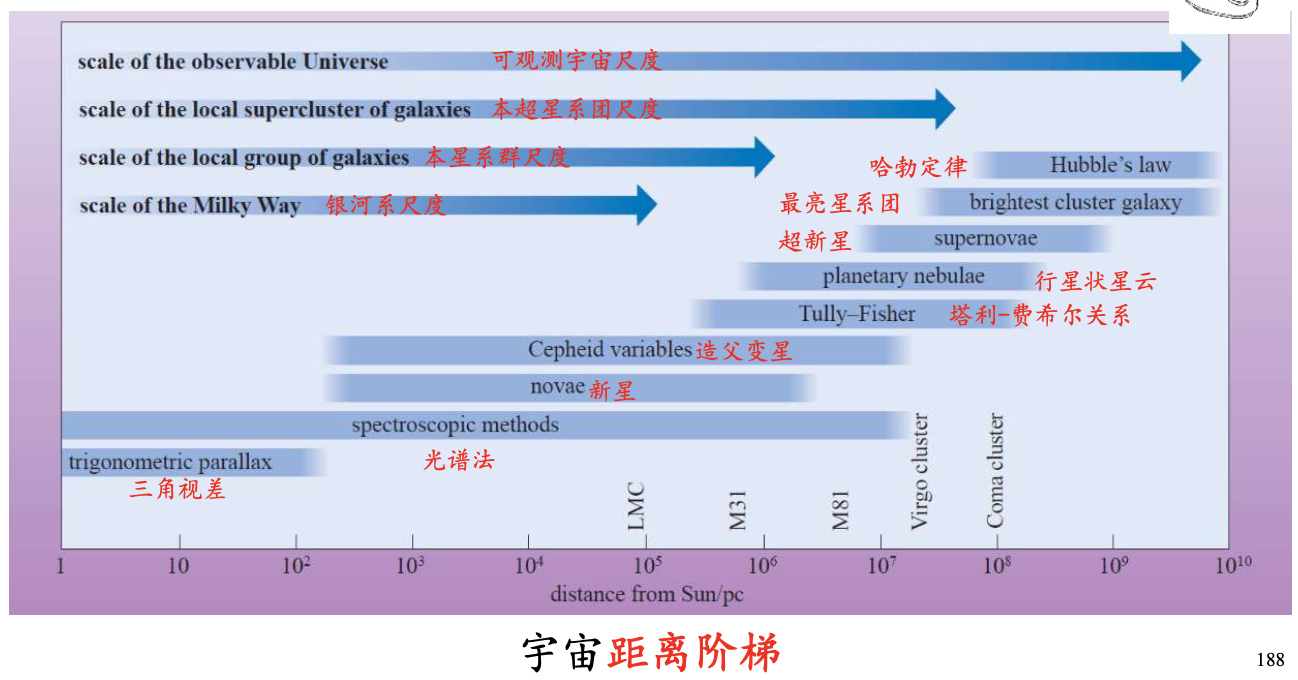
\includegraphics[width=14cm]{figures/figure1_18.png}
\captionsetup{justification=raggedright, singlelinecheck=false}
\caption{距离阶梯。}
\label{距离阶梯。}
\end{figure}

不同的测距方法适用于不同的距离。最基本的三角视差法原理我们在《球面天文》已经介绍过了,通常只适用于$30-500\,\mathrm{pc}$范围内的恒星。它比较依赖望远镜的分辨率。一般来讲,地面望远镜单镜分辨率$\sim10\,\mathrm{mas}$,地面光学/近红外干涉$\sim1\,\mathrm{mas}$,甚长基线干涉$\sim0.1\,\mathrm{mas}$,空间天体测量卫星 Hipparcos 可达$1\,\mathrm{mas}$, 天体测量卫星 Gaia 可达$0.04\,\mathrm{mas}$.有关 Gaia 卫星的原理我们可以在这里提一下,它沿用了 Hipparcos 的扫描空间天体测量原理 (the principle of scanning space astrometry).考虑距离太阳一个天文单位的观测者,恒星视差$\varpi$会造成恒星在天球上的位移,具体形式为$\varpi\sin\theta$,其中$\theta$是天体方向单位矢量与太阳方向单位矢量的夹角。令卫星缓慢自转,当恒星通过卫星搭载的望远镜的视场时,恒星位移垂直自转轴的部分会影响到恒星通过焦平面的时间,因此可将视差测定转换成时间测定。同一视场内$\theta$角差异极小,时间的差值难以测量,因此需要在垂直自转轴的平面上放置两个指向呈一定大角度$\Gamma$的望远镜,比较两个视场内的天体。利用该方法不仅可以实现相对视差测量,还可在不依赖背景天体的情况下实现绝对视差测量。如图\ref{absolute_parallax}左所示,指向 P 点的望远镜测得的沿扫描方向视差位移 (along-scan shift, 简称 AL shift) 等于$0$时,指向 F 点的望远镜测得的沿扫描方向视差位移为$\varpi_{F}\sin\theta\sin\psi=\varpi_{F}\sin\xi\sin\Gamma$,其中$\xi$是太阳方向单位矢量与自转轴的夹角。如此绝对视差测量就变得可行。
\begin{figure}[!htp]
\centering
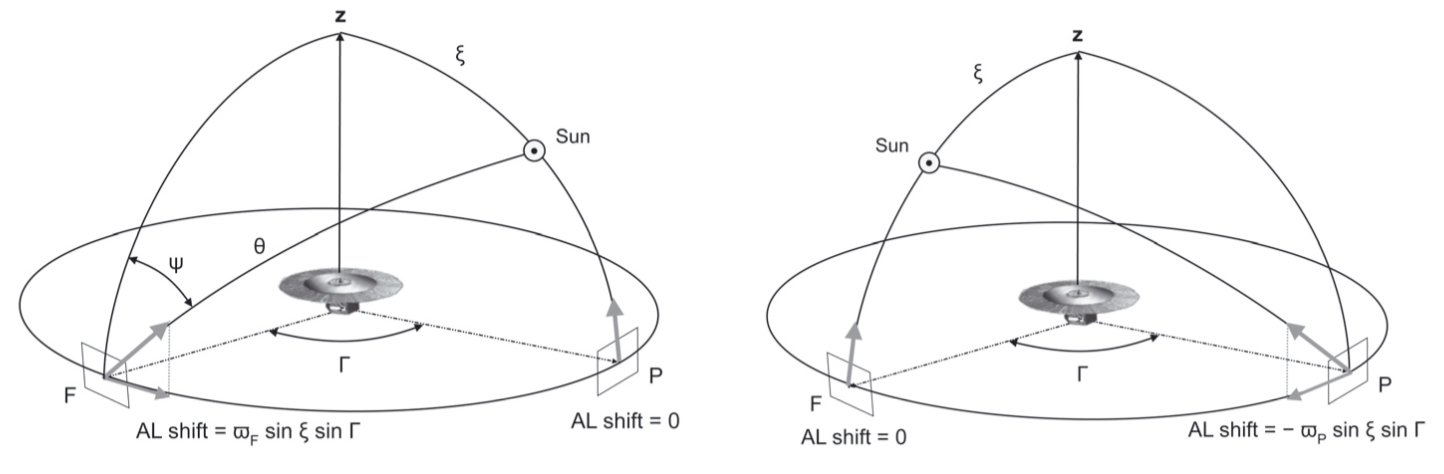
\includegraphics[width=0.9\textwidth]{figures/figure1_19.png}
\captionsetup{justification=raggedright, singlelinecheck=false}
\caption{Gaia 绝对视差测量基本原理图。望远镜的指向相对太阳方向单位矢量处于特定位置时,恒星沿扫描方向视差位移与恒星的绝对视差而非恒星间的相对视差有关,因此可进行绝对视差测量。}
\label{absolute_parallax}
\end{figure}

图\ref{距离阶梯。}中的光谱法一般翻译成分光视差,但它其实和“视差”没关系。视差是一种几何手段,而分光视差可以算是标准烛光法的一种。蜡烛的光度是常量,拿到不同远处看起来则不同,即亮度发生了变化,我们在观测中可以得到天体的亮度,如果再知道它的光度,很容易就能算出距离。唯一的问题是不同天体光度不同,于是我们需要标准烛光。比如造父变星,它是一类光度周期性变化的恒星,且有周光关系:周期越长光度越高。长周期的造父变星光度可达$10^{6}L_{\odot}$,适用于 6000 万光年距离的测距。通过三角视差确定近邻造父变星的距离和实际光度,就可以将其应用在其他造父变星上了。(用下一级阶梯为上一级阶梯定标,所以叫距离阶梯。)\uppercase\expandafter{\romannumeral 1}a 型超新星也可作为标准烛光,原理前文已经解释过了。回到分光视差,我们知道不同质量的主序星会发出不同类型的光谱,观测中可借此区分,所以叫分光。接着假设光谱型相同的恒星光度相同,结合亮度就可测距,因为涉及到测距,所以才叫视差。Tully-Fisher 关系和漩涡星系有关,牛顿引力告诉我们
\begin{equation}
M=\frac{V_{\max}^{2}R}{\mathrm{G}},
\end{equation}
假设不同漩涡星系的质光比都相同,那么$L\propto{}M\propto{}V_{\text{max}}^{2}R$.再假设漩涡星系中心面亮度是常数,那么$L\propto{}R^{2}$,因此$L^{2}\propto{}V_{\max}^{4}R^{2}\propto{}V_{\max}^{4}L,L\propto{}V_{\max}^{4}$.通过光谱红移确定自转速度就可确定光度进而测距。

哈勃定律测距需要注意的是,星系的视向速度不仅来自空间膨胀,还来自局域引力作用(别的天体拖拽)下星系相对空间本身的运动速度(本动速度)。即
\begin{equation}
V_{\mathrm{r}}=H_{0}d+V_{\text{pec}}.
\end{equation}
富团内本动速度高达$1500\,\mathrm{km\cdot s^{-1}}$.
\printbibliography
\end{document}
